\documentclass[11pt,openany]{book}
\raggedbottom

% Load packages
\usepackage[utf8]{inputenc} % for unicode input
\usepackage{microtype}
\usepackage{bm}
\usepackage{enumitem}
\usepackage{geometry} % for page layout
\usepackage{hyperref} % for hyperlinks
\usepackage{tocbibind} % includes the bibliography in the table of contents
\usepackage{amsmath, amsfonts, amssymb, amsthm} % for advanced math formatting
\usepackage{lipsum} % generates filler text
\usepackage{fancyhdr}
\usepackage[table]{xcolor} % for cell coloring
\usepackage{graphicx} % for including images
\usepackage{booktabs} % for professional looking tables
\usepackage[normalem]{ulem} % for underlining
\usepackage[document]{ragged2e} % for text alignment
\usepackage{tikz} % for drawing
\usepackage{algorithm}
\usepackage{algpseudocode}
\usepackage{wrapfig}
\usepackage{circuitikz}
\usepackage{caption}
\usepackage{venndiagram}
\usepackage{multicol}
\usepackage{listings}
\usepackage{adjustbox}
\usepackage{multirow}


% TikZ libraries
\usetikzlibrary{circuits.logic.US, arrows.meta, positioning, calc, fit, decorations.markings, math}

% Document geometry (page size, margins)
\geometry{a4paper, left=20mm, right=20mm, top=25mm, bottom=30mm}

% Custom page style for centered page numbers
\pagestyle{fancy}
\fancyhf{} % Clear all header and footer fields
\fancyhead[RE]{\leftmark} % Left Even pages - Chapter number and name
\fancyhead[RO]{Notes by Ali EL AZDI} % Right Odd pages - Custom message
\fancyfoot[CE,CO]{\thepage} % Centered page number in the footer for both even and odd pages
\renewcommand{\headrulewidth}{0pt}
\renewcommand{\footrulewidth}{0pt}

% Custom commands
\newcommand*\xor{\oplus}
\newcommand{\minidash}{\text{-}}

% Custom spacing command
\makeatletter
\newcommand{\vspacer}[1]{%
  \ifvmode
    \vskip#1\relax
  \else
    \@bsphack
    \vadjust{\vskip#1\relax}
    \@esphack
  \fi
}
\makeatother

%%%%%%%%%%%%%%%%%%% Verilog CODE STYLING %%%%%%%%%%%%%%%%%%%%%%%%%%%%%
\definecolor{keywordcolor}{rgb}{0.5,0.0,0.33}
\definecolor{backgroundcolor}{rgb}{0.95,0.95,1.0}
\definecolor{commentcolor}{rgb}{0.129,0.384,0.529}
\definecolor{stringcolor}{rgb}{0.16,0.00,1.00}
\definecolor{rulecolor}{rgb}{0.46,0.43,0.5}
\definecolor{codegray}{rgb}{0.5,0.5,0.5}

\lstdefinestyle{verilogstyle}{
  language=Verilog,
  basicstyle=\ttfamily\footnotesize,
  backgroundcolor=\color{backgroundcolor},
  commentstyle=\color{commentcolor}\ttfamily, % Add \ttfamily to ensure comments are in typewriter font
  morecomment=[l][\color{commentcolor}\ttfamily]{//}, % Line comment in Verilog
  morecomment=[s][\color{commentcolor}\ttfamily]{/*}{*/}, % Block comments in Verilog
  morekeywords={module, input, output, wire, endmodule, endcase, default, tri, assign, always, if, else, begin, end, case, endcase, parameter}, % Add Verilog keywords
  keywordstyle=\color{keywordcolor},
  stringstyle=\color{stringcolor},
  showstringspaces=false,
  frame=single,
  rulecolor=\color{rulecolor}, % Frame color
  breaklines=true,
  numbers=left,
  numberstyle=\tiny\color{codegray},
  tabsize=2
}

\lstnewenvironment{verilog}
  {\lstset{style=verilogstyle}}
  {}

%%%%%%%%%%%%%%%%%%% C CODE STYLING %%%%%%%%%%%%%%%%%%%%%%%%%%%%%
\definecolor{ckeywordcolor}{rgb}{0.8,0.1,0.1}
\definecolor{cbackgroundcolor}{rgb}{0.95,0.95,0.95}
\definecolor{ccommentcolor}{rgb}{0.0,0.5,0.0}
\definecolor{cstringcolor}{rgb}{0.1,0.1,0.8}
\definecolor{crulecolor}{rgb}{0.5,0.5,0.5}
\definecolor{ccodegray}{rgb}{0.6,0.6,0.6}

\lstdefinestyle{cstyle}{
  language=C,
  basicstyle=\ttfamily\footnotesize,
  backgroundcolor=\color{cbackgroundcolor},
  commentstyle=\color{ccommentcolor}\ttfamily,
  keywordstyle=\color{ckeywordcolor},
  stringstyle=\color{cstringcolor},
  showstringspaces=false,
  frame=single,
  rulecolor=\color{crulecolor},
  breaklines=true,
  numbers=left,
  numberstyle=\tiny\color{ccodegray},
  tabsize=2
}

\lstnewenvironment{cc}
  {\lstset{style=cstyle}}
  {}

%%%%%%%%%%%%%%%%%%% Assembly CODE STYLING %%%%%%%%%%%%%%%%%%%%%%%%%%%%%
\definecolor{akeywordcolor}{rgb}{0.0, 0.2, 0.4}
\definecolor{abackgroundcolor}{rgb}{0.98, 0.99, 1.0}
\definecolor{acommentcolor}{rgb}{0.0, 0.4, 0.6}
\definecolor{astringcolor}{rgb}{0.2, 0.4, 0.8}
\definecolor{arulecolor}{rgb}{0.6, 0.7, 0.8}
\definecolor{acodegray}{rgb}{0.3, 0.4, 0.5}

\lstdefinestyle{assembly}{
  language=[x86masm]Assembler,
  basicstyle=\ttfamily\footnotesize,
  backgroundcolor=\color{abackgroundcolor},
  commentstyle=\color{acommentcolor}\ttfamily,
  keywordstyle=\color{akeywordcolor},
  stringstyle=\color{astringcolor},
  showstringspaces=false,
  frame=single,
  rulecolor=\color{arulecolor},
  breaklines=true,
  numbers=left,
  numberstyle=\tiny\color{acodegray},
  tabsize=2,
  morekeywords={li, and, add, addi, srli, bne}
}

\lstnewenvironment{assembly}
  {\lstset{style=assembly}}
  {}

%%%%%%%%%%%%%%%%%%%%%%%%%%%%%%%%%%%%%%%%%%%%%%%%%%%%%%%%
%%%%%%%%%%%%%%%%%%% JAVA CODE STYLING %%%%%%%%%%%%%%%%%%%%%%%%%%%%%
\definecolor{javakeywordcolor}{rgb}{0.0, 0.0, 0.5}
\definecolor{javabackgroundcolor}{rgb}{0.95, 0.95, 0.95}
\definecolor{javacommentcolor}{rgb}{0.0, 0.5, 0.0}
\definecolor{javastringcolor}{rgb}{0.6, 0.0, 0.0}
\definecolor{javarulecolor}{rgb}{0.5, 0.5, 0.5}
\definecolor{javagray}{rgb}{0.6, 0.6, 0.6}

\lstdefinestyle{javastyle}{
  language=Java,
  basicstyle=\ttfamily\footnotesize,
  backgroundcolor=\color{javabackgroundcolor},
  commentstyle=\color{javacommentcolor}\ttfamily,
  keywordstyle=\color{javakeywordcolor},
  stringstyle=\color{javastringcolor},
  showstringspaces=false,
  frame=single,
  rulecolor=\color{javarulecolor},
  breaklines=true,
  numbers=left,
  numberstyle=\tiny\color{javagray},
  tabsize=2,
  morekeywords={class, public, private, protected, extends, implements, interface, import, package, new, return, void, static}
}

\lstnewenvironment{java}
  {\lstset{style=javastyle}}
  {}

%%%%%%%%%%%%%%%%%%%%%%%%%%%%%%%%%%%%%%%%%%%%%%%%%%%%%%%%
% Document begins
\begin{document}


% Title Page
\begin{titlepage}
    \centering
    \vspace*{1cm}
    \Huge
    Computer Architecture \newline
    \vspace{10px}
    \LARGE IN BA3 - Paolo IENNE
    \vspace*{10px}
    \newline
    \Large Notes by Ali EL AZDI

    \vfill
    \large
    September 11, 2024
\end{titlepage}

\begin{center}
    \vspace*{1cm}
    \textbf{Introduction}
    \newline
    \paragraph[short]{}{This document is designed to offer a LaTeX-styled overview of the Computer Architecture course, emphasizing brevity and clarity. Should there be any inaccuracies or areas for improvement, please reach out at ali.elazdi@epfl.ch for corrections. For the latest version, check my GitHub repository.}
    \newline
   \url{
        https://github.com/elazdi-al/comparch/blob/main/main.pdf
    }
    \newline
\end{center}

% Table of Contents
\tableofcontents

 % Including chapter0.tex from chapters folder
\chapter{Part I(a) - ISA Reminder, Assembly Language, Compiler - W 1.1}
\textbf{hum...welcome back} \newline
\textit{In the first part of the course, professor introduced (for motivational purposes) how computer architecture, specifically processors, have become essential to our lives, and how the field is growing exponentially. (didn't think it was essential to mention here...)}

\section{From High Level Languages to Assembly Language}
\subsection{High Level Languages}
\textit{When talking about programming we usually think of programs that look like this\dots} \newline \vspace*{5px}

\begin{minipage}[htp]{0.4\textwidth} % Use \textwidth to ensure it spans the page width
\begin{cc}
int data = 0x00123456;
int result = 0;
int mask = 1;
int count = 0;
int temp = 0;
int limit = 32;
do {
    temp = data & mask;
    result = result + temp;
    data = data >> 1;
    count = count + 1;
} while (count != limit);
\end{cc}
\end{minipage}
\hfill
\vline
\hfill
\begin{minipage}[htp]{0.4\textwidth}
    \centering
    \begin{tabular}{|c|c|}
        \hline
        \textbf{name} & \textbf{value} \\ \hline
        data       & 0x00123456  \\ \hline
        result     & 0           \\ \hline
        mask       & 1           \\ \hline
        count      & \dots       \\ \hline
        temp       &             \\ \hline
        limit      &             \\ \hline
        \dots      &             \\ \hline
        my\_float  & 3.141529    \\ \hline
        a\_string  & Hello world! \\ \hline
        \end{tabular}
\end{minipage}

\subsection{Assembly Language}
We use this code because it enables us to build a \textit{Finite State Machine}, which isn't feasible with C code. This language provides a more rigid format with a sequence of numbered instructions, an \textit{opcode}, predefined variable names, and the ability to \textbf{jump between lines}.
\newpage
\begin{center}
    \begin{assembly}
    li x1, 0x00123456
    li x2, 0
    li x3, 1
    li x4, 0
    li x5, 0
    li x6, 32
loop: and x5, x1, x3
    add x2, x2, x5
    srli x1, x1, 1
    addi x4, x4, 1
    bne x4, x6, loop
    \end{assembly}
\end{center}

\section{Processors}
\textbf{Remember, a processor can be decomposed into five components:} \newline
\begin{itemize}[noitemsep]
    \item[-] \textbf{ALU (Arithmetic and Logic Unit)}: Performs arithmetic and logical operations.
    \item[-] \textbf{Register File}: Stores data temporarily for quick access during processing.
    \item[-] \textbf{Memory}: Holds data and instructions needed by the processor.
    \item[-] \textbf{Control Logic}: Directs the operation of the processor by coordinating the other components.
    \item[-] \textbf{PC (Program Counter)}: Keeps track of the address of the next instruction to be executed.
    \item[-] \textbf{Instruction Memory}: Stores the program instructions that the processor will execute.
\end{itemize}
\begin{center}
    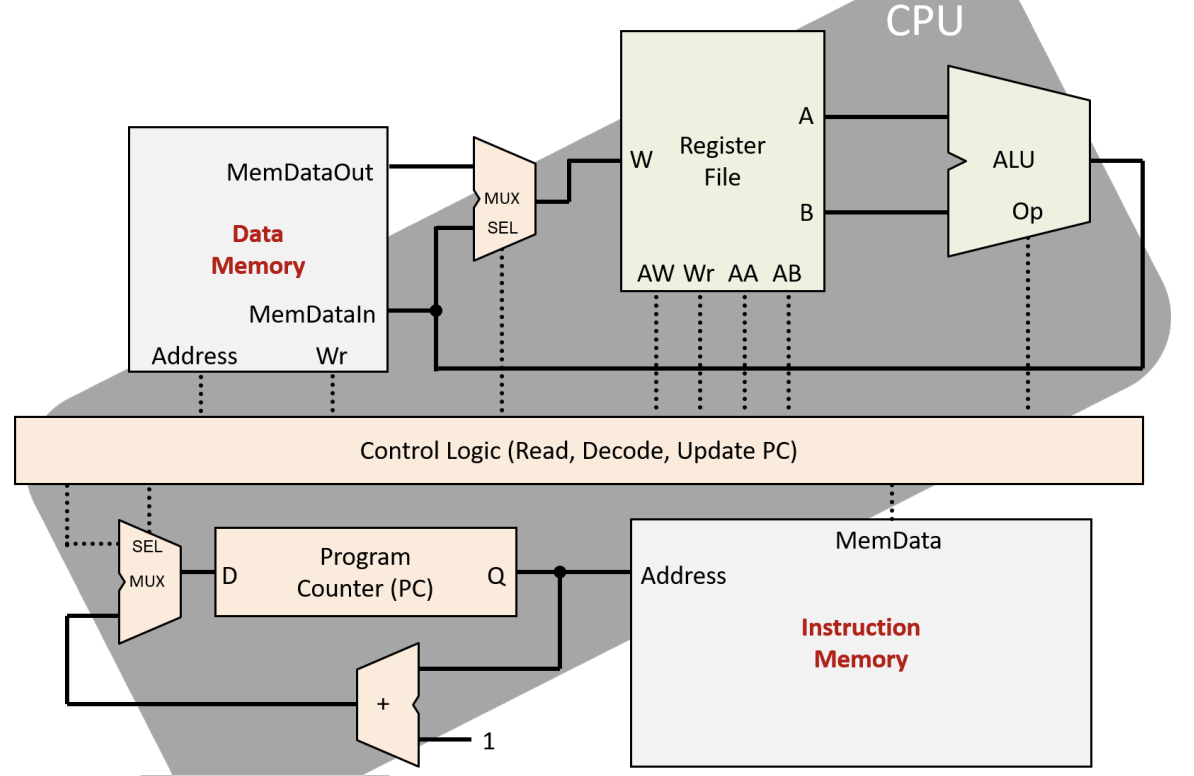
\includegraphics[width=0.5\textwidth]{chapters/chapter1a/images/processor.png}
\end{center}

We may distinguish three types of general operations made by the processor: \newline
\subsubsection*{Encoding}
\begin{center}
    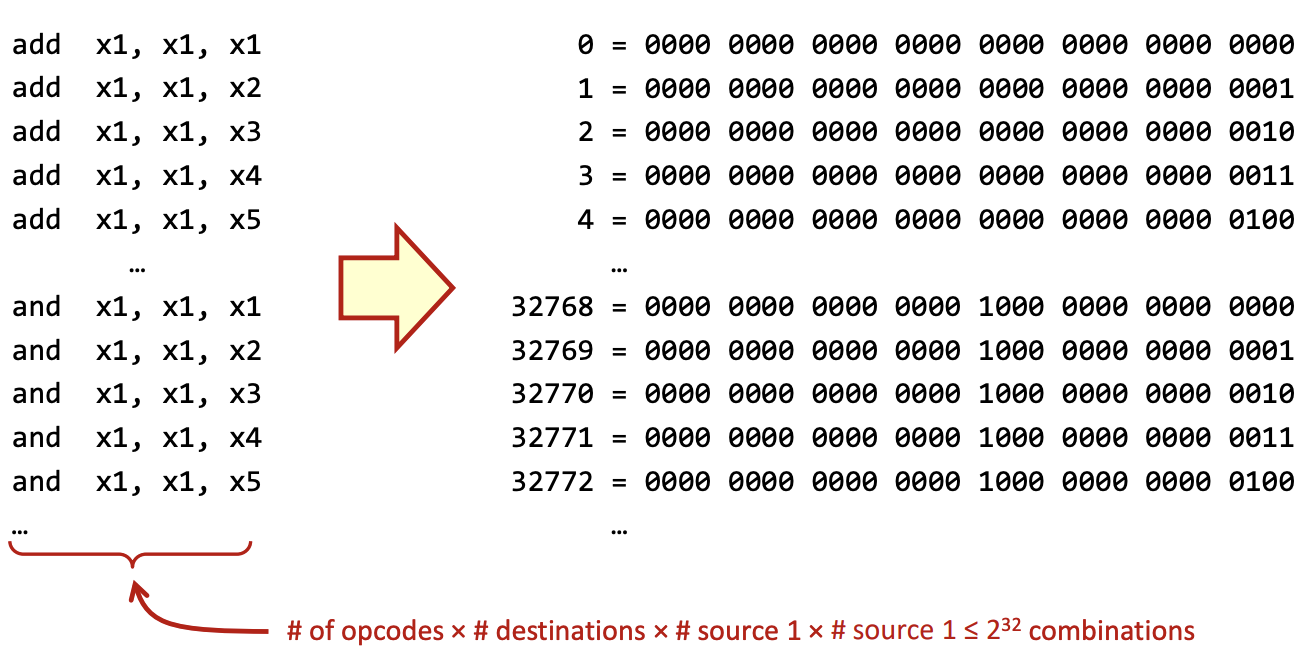
\includegraphics[width=0.65\textwidth]{chapters/chapter1a/images/encoding.png}
\end{center}
\subsubsection*{Fetching}
\begin{center}
    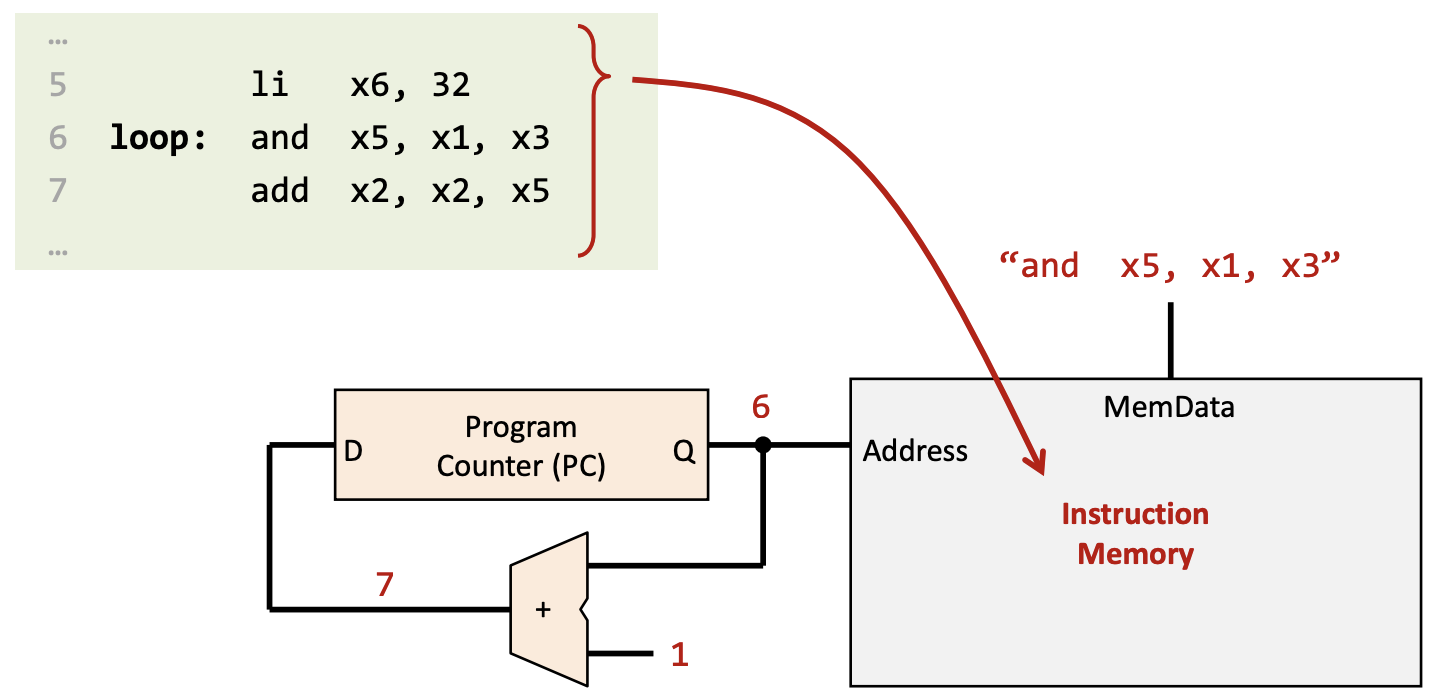
\includegraphics[width=0.65\textwidth]{chapters/chapter1a/images/fetching.png}
\end{center}
\subsubsection*{Executing}
\begin{center}
    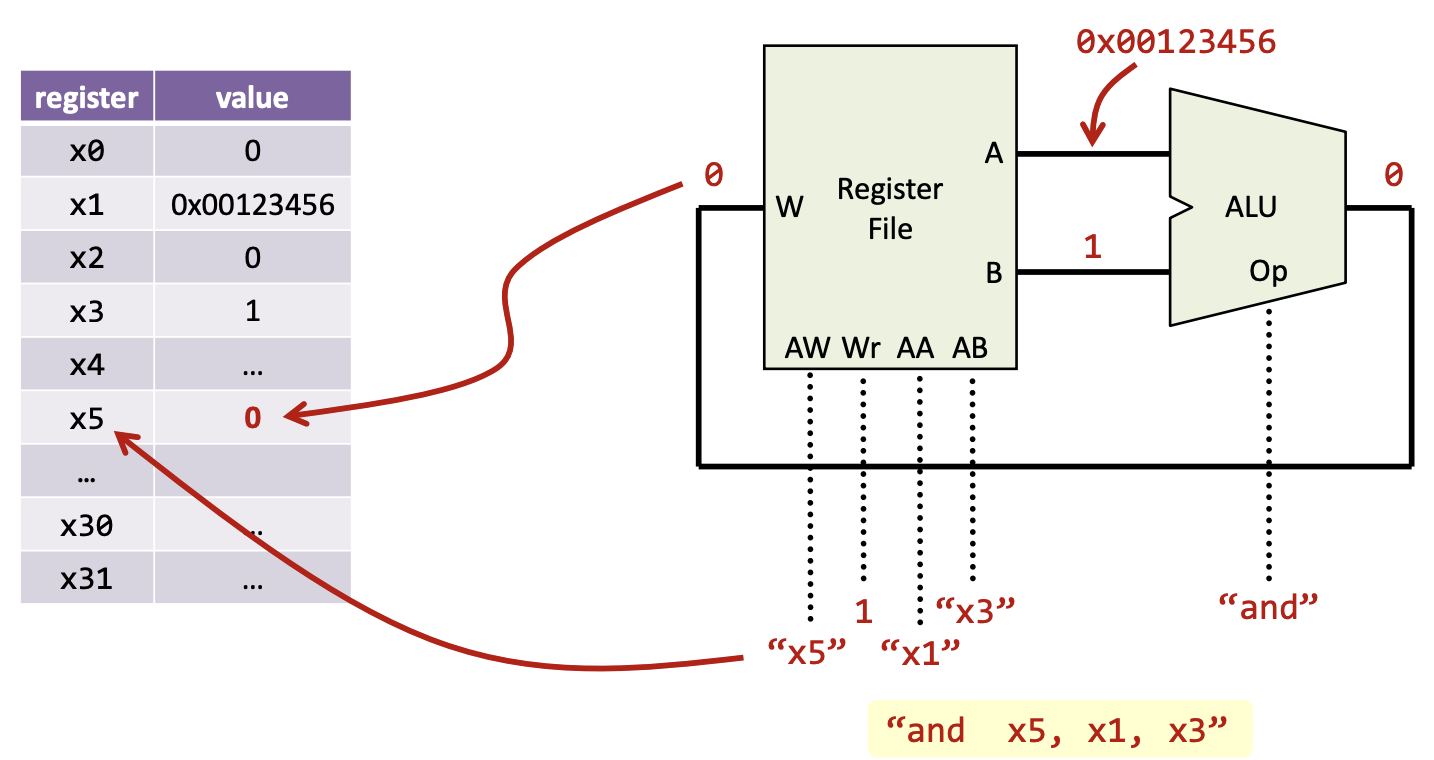
\includegraphics[width=0.65\textwidth]{chapters/chapter1a/images/executing.png}
\end{center}


\section{Joint or Disjoint Program and Data Memories}
\textit{There are two main types of architectures one called the Harvard Architecture (Where the data and the memory are seperate) and pne called Unified Architecture (where data is shared with the program memory)} \newline
\vspace*{10px}
\begin{minipage}[htp]{0.4\textwidth}
    \texttt{Harvard Architecture} \newline
    \vspace*{2px}
    \centering
    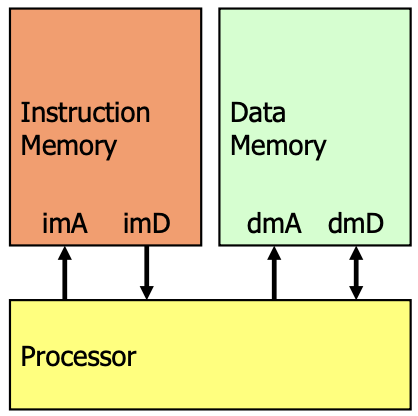
\includegraphics[width=0.6\textwidth]{chapters/chapter1a/images/harvard.png}
\end{minipage}
\hfill
\vline
\hfill
\begin{minipage}[htp]{0.4\textwidth}
    \texttt{Unified Architecture} \newline    
    \vspace*{2px}

    \centering
    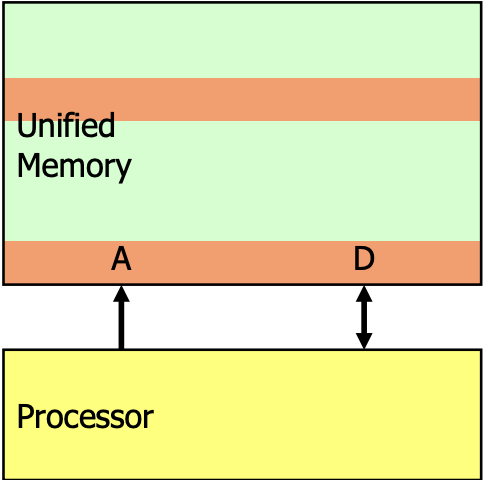
\includegraphics[width=0.6\textwidth]{chapters/chapter1a/images/unified.png}
\end{minipage}
\newpage
\section{The Encoding problem}
\textit{We may ask ourselves how we encode assembly written instructions into actual 0s and 1s.} \newline
\subsection{The Stupid Solution}
\textit{Now, the professor throws out the "stupid idea"(his words) of just counting all possible instructions, assigning a number to each one, and writing the numbers in binary. The problem with such a method is that the number of instructions could grow exponentially, requiring an unmanageable number of bits to represent each one, leading to inefficiency.} \newline 
\begin{center}
    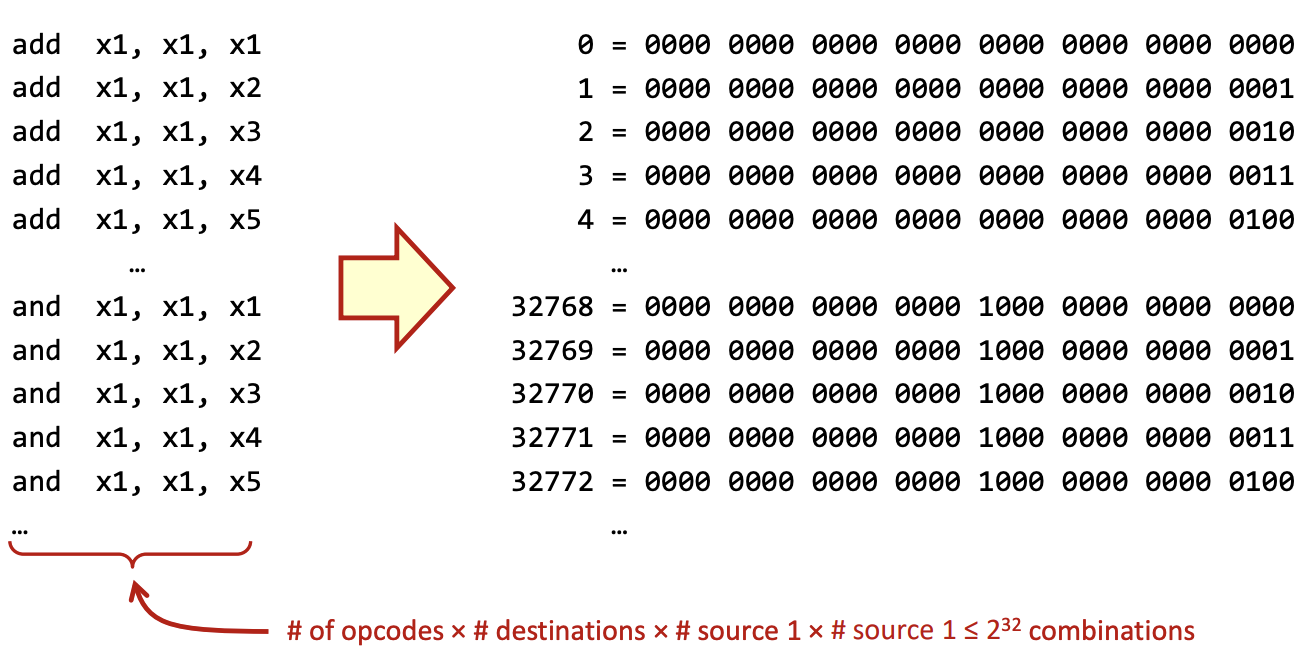
\includegraphics[width=0.7\textwidth]{chapters/chapter1a/images/encoding.png}
    \centering
    \textbf{"stupid solution"}
\end{center}

\subsection{RISC-V Encoding (The Solution)}
\textbf{Instead, the chosen solution is to use an instruction set encoding where instructions are grouped into classes, each with a fixed format optimizing both memory usage and processing speed by limiting the number of bits required to represent instructions.} \newline
\begin{center}
    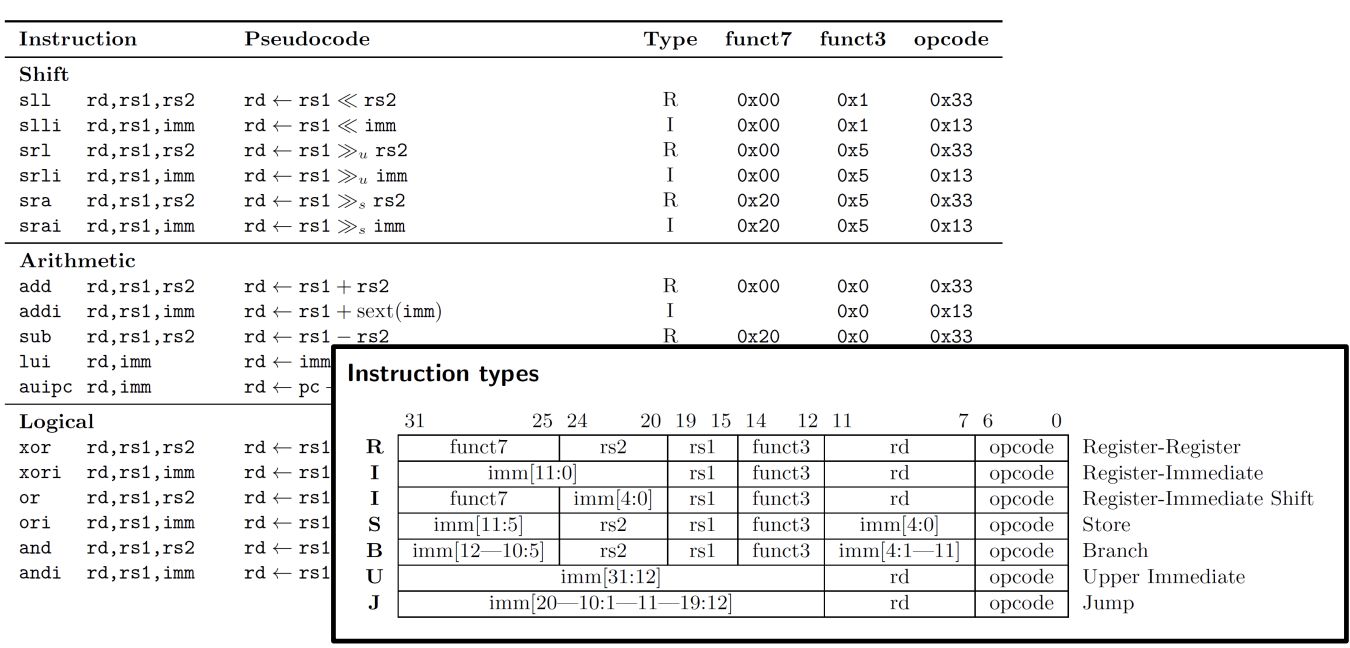
\includegraphics[width=0.7\textwidth]{chapters/chapter1a/images/riscv.png}
    \centering
    \textbf{RISC-V encoding}
\end{center}

\newpage
\subsection{Automating this process}
\textit{Now to automate the processes of decoding assembler code into machine code we use an \textbf{Assembler}, and to automate the process of decoding a higher level language to assembler we use a \textbf{Compiler}}. \newline
\subsubsection{Assembler}
\textit{The program that does this is called an assembler. It takes the assembly code and converts it into machine code.} \newline
\begin{center}
    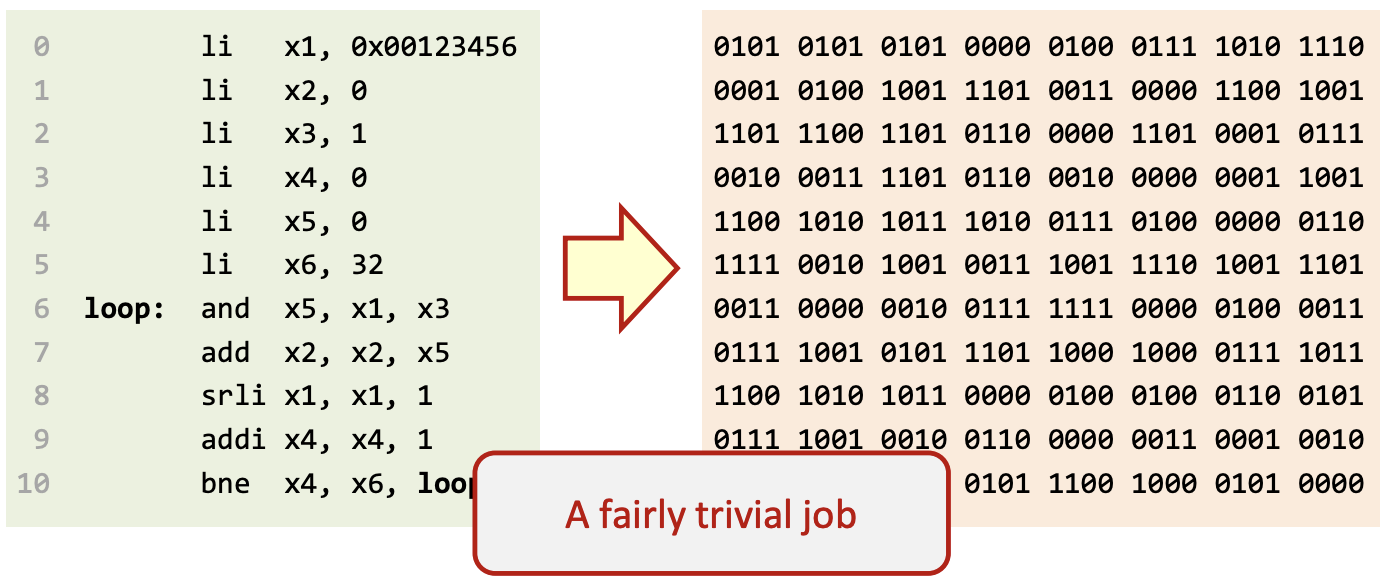
\includegraphics[width=0.7\textwidth]{chapters/chapter1a/images/assembler.png}
    \centering
    \textbf{Assembly}
\end{center}
\subsubsection{Compiler}
A compiler is a program that translates high-level source code written in languages like C or Java into machine code or an intermediate representation. 
\begin{center}
    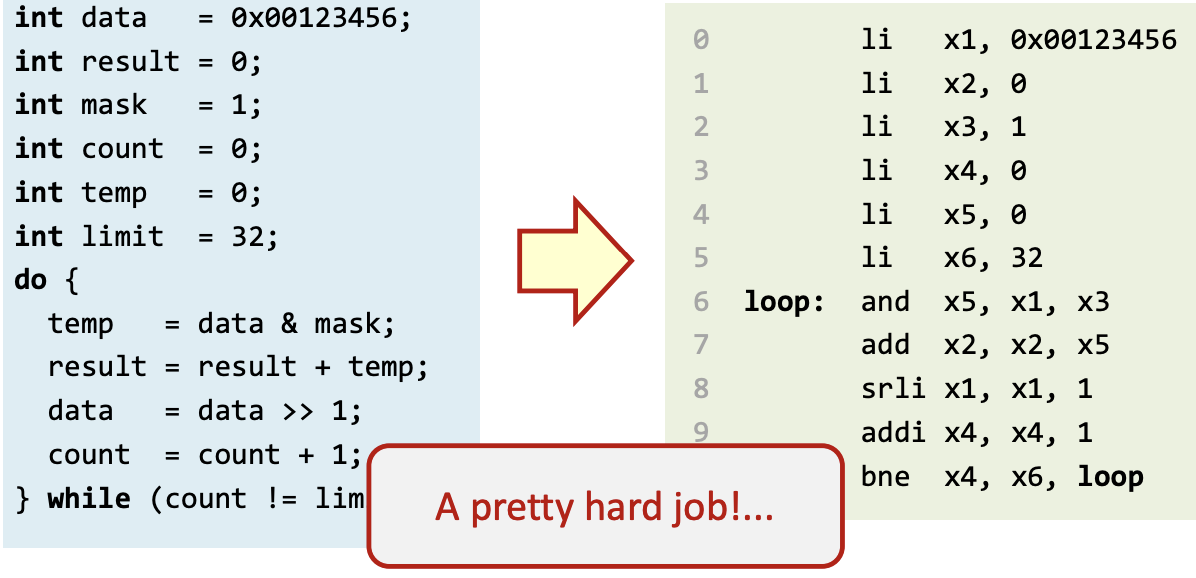
\includegraphics[width=0.7\textwidth]{chapters/chapter1a/images/compiler.png}
    \centering
    \textbf{Compilation}
\end{center}


\section{ISA (Instruction Set Architecture)}
\textit{The ISA is the interface between the hardware and the software. It defines the instructions that a processor can execute, as well as the format of those instructions.} \newline
\begin{center}
    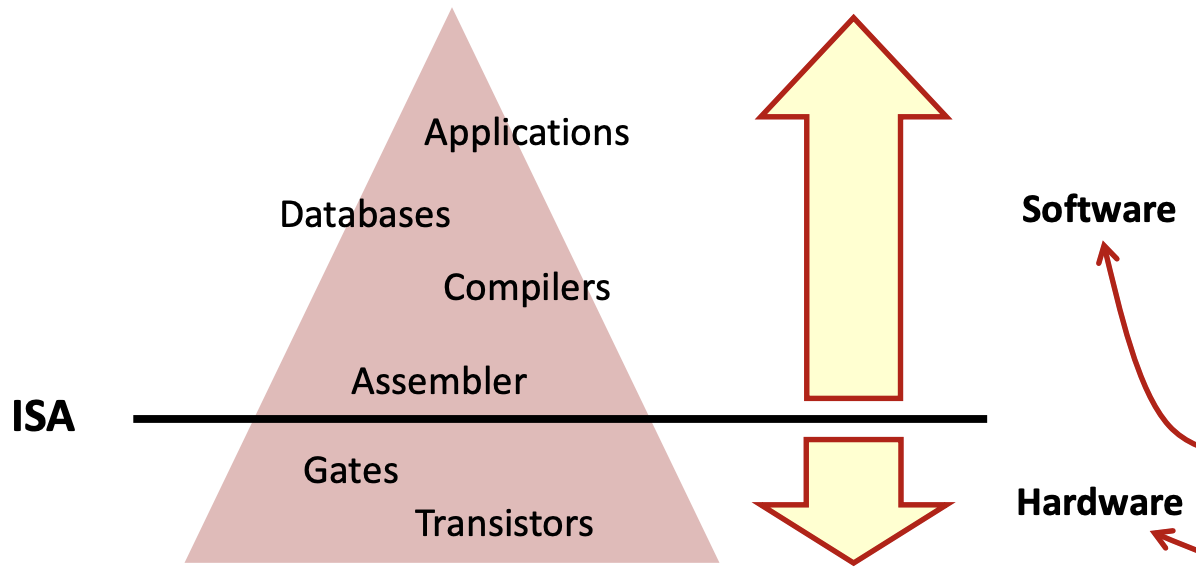
\includegraphics[width=0.65\textwidth]{chapters/chapter1a/images/isa.png}
    \centering
\end{center} % Including chapter0.tex from chapters folder
\chapter{Part I(b) - ISA, Functions, and Stack - W 1.2}
\section{Arithmetic and Logic Instructions in RISCV}
\textit{Bellow some examples of RISCV instructions:} \\
\textbf{Two Operands Instructions} \\
\vspace*{10px}
\begin{minipage}{0.4\textwidth}
\begin{assembly}
sll  x5, x5, x9
add  x6, x5, x7
xor  x6, x6, x8
slt  x8, x6, x7
\end{assembly}
\end{minipage}%
\hfill
\vline
\hfill
\begin{minipage}{0.5\textwidth}
\small
\textit{Shift x5 left by x9 positions $\rightarrow$ x5} \\
\textit{Add x5 and x7 $\rightarrow$ x6} \\
\textit{Logic XOR bitwise x6 and x8 $\rightarrow$ x6} \\
\textit{Set x8 to 1 if x6 is lower than x7, otherwise to 0}
\end{minipage}

\textbf{Arithmetic Instructions} \\
\vspace*{10px}
\begin{minipage}{0.4\textwidth}
\begin{assembly}
slli x5, x5, 3
addi x6, x5, 72
xori x6, x6, -1
slti x8, x6, 321
\end{assembly}
\end{minipage}%
\hfill
\vline
\hfill
\begin{minipage}{0.5\textwidth}
\small
\textit{Shift x5 left of 3 positions $\rightarrow$ x5} \\
\textit{Add 72 to x5 $\rightarrow$ x6} \\
\textit{Logic XOR bitwise x6 and 0xFFFFFFFF $\rightarrow$ x6} \\
\textit{Set x8 to 1 if x6 is lower than 321, to 0 otherwise} \\
\end{minipage} \\
\textbf{Here, you may ask yourself, why are all immediates (constants) writtent on a maximum of 12bits?} \\
\subsection{Constants must be encoded on 12 bits}
\textit{As you may see here, all instructions encode immediates on 12 bits.}
\begin{center}
    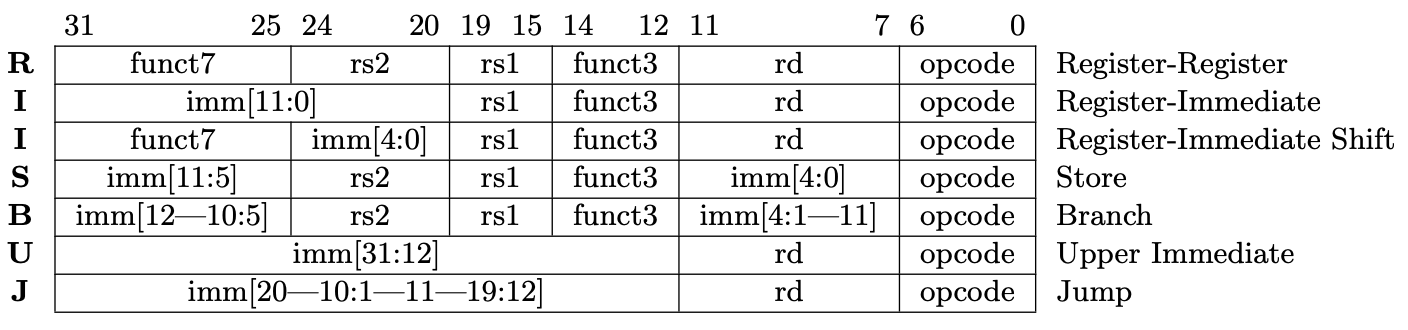
\includegraphics[width=0.8\textwidth]{chapters/chapter1b/images/riscv.png}
\end{center}

\subsection{Assembler Directives} \textit{Assembler directives help write cleaner and more readable code. The code snippets on the left and right below are equivalent.}

\begin{center} 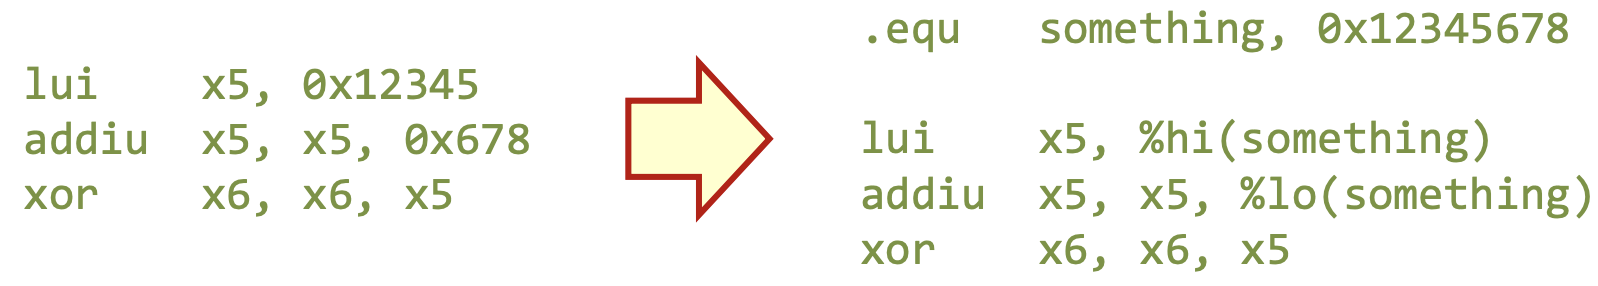
\includegraphics[width=0.65\textwidth]{chapters/chapter1b/images/directives.png} \end{center}

The left-hand side code snippet shows an assembly sequence where a 32-bit constant value (\texttt{0x12345678}) is loaded into a register (\texttt{x5}). Since immediate values are 16-bit limited, this requires splitting the 32-bit value into two instructions: 

\begin{itemize}
    \item[-] The first instruction, \texttt{lui}, loads the upper 16 bits (\texttt{0x12345}) into the register \texttt{x5}.
    \item[-] The second instruction, \texttt{addiu}, adds the lower 16 bits (\texttt{0x678}) to \texttt{x5}, completing the full 32-bit value in the register.
\end{itemize}

\textit{This approach, while functional, can become cumbersome when dealing with multiple constants, making the code less readable and harder to maintain. \\
} 
\vspace*{5px}
The right-hand side shows the same functionality but makes use of assembler directives, specifically the \texttt{.equ} directive to define a label (\texttt{something}) for the constant \texttt{0x12345678}. Using the \texttt{\%hi()} and \texttt{\%lo()} pseudo-instructions, the assembler automatically splits the constant into its upper and lower parts:

\begin{itemize}
    \item[-] The \texttt{\%hi(something)} loads the upper 16 bits into \texttt{x5}.
    \item[-] The \texttt{\%lo(something)} adds the lower 16 bits to \texttt{x5}.
\end{itemize}

This method enhances code clarity and maintainability, especially when working with multiple constants, by using human-readable labels instead of raw numeric values. The assembler handles the details of splitting the 32-bit constant into its upper and lower parts.
\begin{center} 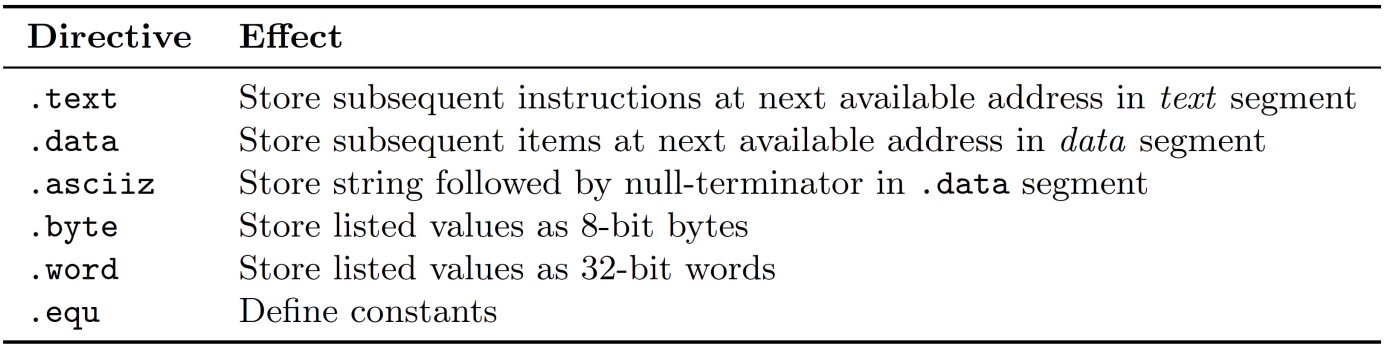
\includegraphics[width=0.65\textwidth]{chapters/chapter1b/images/directives2.png} \end{center}

\subsection{The \texttt{x0} Register} 
\textit{The \texttt{x0} register is hardwired to 0 and cannot be changed.} \ \textit{Any attempt to write into \texttt{x0} will have no effect.}

\texttt{Why is this useful?} \\
One common application is in introducing wait delays during program execution. By leveraging the fixed nature of \texttt{x0}, it simplifies certain instructions that require an immediate zero value.

\section{PseudoInstructions}
\textit{PseudoInstructions simplify commands involving the \texttt{x0} register by creating easier-to-use alternatives.} \newline
\begin{center}
        \begin{tabular}{|c|c|c|}
        \hline
        \textbf{Pseudoinstruction} & \textbf{Base Instruction(s)} & \textbf{Meaning} \\ \hline
        \texttt{nop}               & \texttt{addi x0, x0, 0}      & No operation     \\ \hline
        \texttt{li rd, immediate}  & Myriad sequences             & Load immediate   \\ \hline
        \texttt{mv rd, rs}         & Myriad sequences             & Copy register    \\ \hline
        \texttt{not rd, rs}        & \texttt{xori rd, rs, -1}     & One's complement \\ \hline
        \texttt{neg rd, rs}        & \texttt{sub rd, x0, rs}      & Two's complement \\ \hline
        \texttt{seqz rd, rs}       & \texttt{sltiu rd, rs, 1}     & Set if = zero    \\ \hline
        \texttt{snez rd, rs}       & \texttt{sltu rd, x0, rs}     & Set if $\neq$ zero    \\ \hline
        \texttt{sltz rd, rs}       & \texttt{slt rd, rs, x0}      & Set if < zero    \\ \hline
        \texttt{sgtz rd, rs}       & \texttt{slt rd, x0, rs}      & Set if > zero    \\ \hline
        \end{tabular}
\end{center} 
The term \textit{myriad sequences} refers to a series of instructions that together achieve the functionality of a single pseudoinstruction, such as using \texttt{lui} and \texttt{addi} to implement \texttt{li rd, immediate}.

\textbf{According to the professor li should be called \texttt{mvi} (as move immediate).}

\subsection{Control flow instructions}
\textit{Control flow instructions are used to change the order of execution of instructions are a kind of pseudo-instructions.}
\begin{assembly}
    li x1, 0x00123456
    li x2, 0
    li x3, 1
    li x4, 0
    li x5, 0
    li x6, 32
loop: and x5, x1, x3
    add x2, x2, x5
    srli x1, x1, 1
    addi x4, x4, 1
    bne x4, x6, loop
\end{assembly}

\subsection{If-Then-Else}
\begin{minipage}[htp]{0.4\textwidth}
\begin{cc}
if (x5 == 72) {
    x6 = x6 + 1;
    } else {
    x6 = x6 - 1;
}
\end{cc}    
\end{minipage}
\hfill
\vline
\hfill
\begin{minipage}[htp]{0.4\textwidth}
\begin{assembly}
.text
    li x7, 72
    beq x5, x7, then_clause
else_clause:
    addi x6, x6, -1
    j end_if
then_clause:
    addi x6, x6, 1
end_if:
\end{assembly}
\end{minipage} \\
\vspace*{5px}
\textit{As seen here, beqi does not exist in RISCV, instead we use \texttt{beq} and \texttt{li} to achieve the same result.}
\subsection{Jumps and Branches}
A common but not universal distinction exists between \emph{jumps} and \emph{branches}. In RISC-V (inherited from MIPS and used by SPARC, Alpha, etc.), jumps refer to unconditional control transfer instructions, while branches refer to conditional control transfer instructions. However, not all architectures follow this convention. For instance, in x86, all control transfer instructions are considered jumps, such as \texttt{JMP}, \texttt{JZ}, \texttt{JC}, and \texttt{JNO}.

\subsection{Comparaisions}
\textit{The processor implements only $<$ and $>$, and the assembler “creates” $\leq$ and $\geq$.}

\begin{center}
    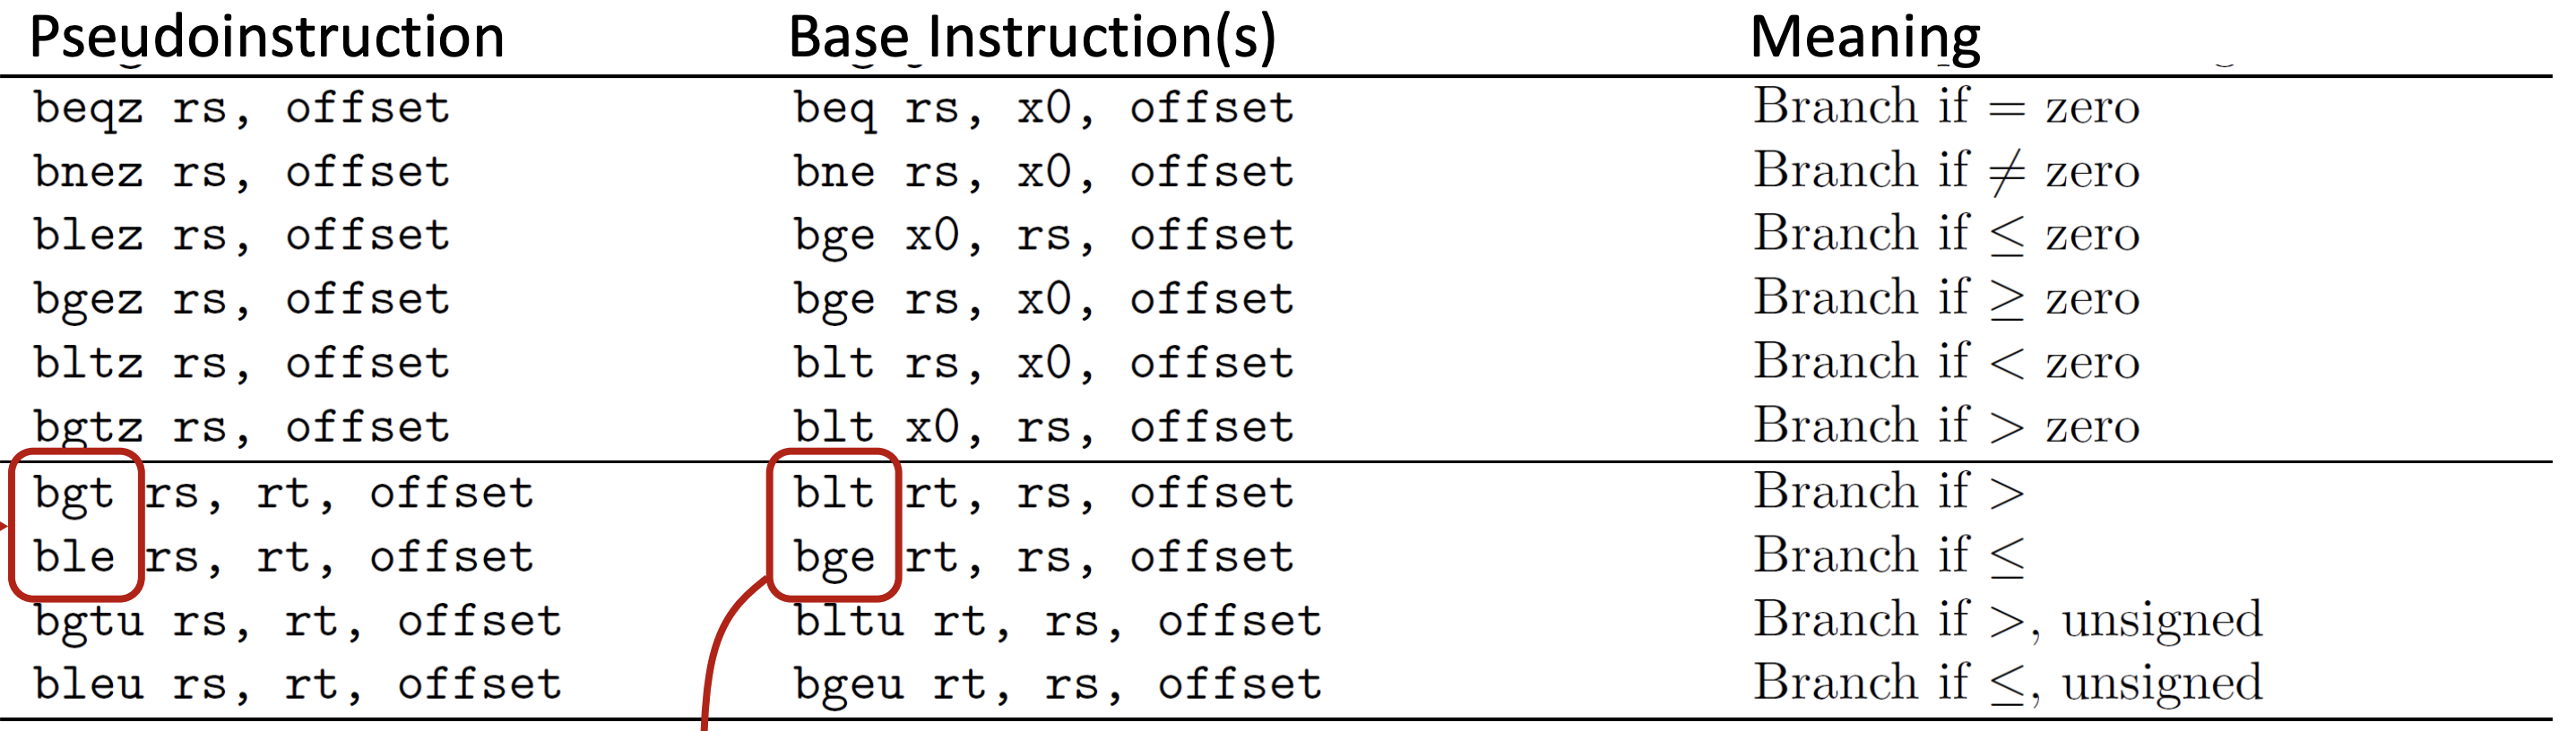
\includegraphics[width=0.75\textwidth]{chapters/chapter1b/images/comp.png}
\end{center}
\subsection{Do-While}
\textit{Do-while loops look like this (we obviously use control flow instructions here).} \\
\begin{minipage}[htp]{0.4\textwidth}
\begin{cc}
do {
    x5 = x5 >> 1;
    x6 = x6 + 1;
} while (x5 != 0);
\end{cc}    
\end{minipage}
\hfill
\vline
\hfill
\begin{minipage}[htp]{0.4\textwidth}
\begin{assembly}
.text
loop:
    srli x5, x5, 1
    addi x6, x6, 1
    bnez x5, loop
\end{assembly}
\end{minipage}

\section{Functions}
\textit{In higher-level programming languages, functions (routines, subroutines, procedures, methods, etc.) are used to encapsulate code and make it reusable. } \\
\textbf{Calling a function involves these steps:}
\begin{enumerate}
    \item Place arguments where the called function can access them.
    \item Jump to the function.
    \item Acquire storage resources the function needs.
    \item Perform the desired task of the function.
    \item Communicate the result value back to the calling program.
    \item Release any local storage resources.
    \item Return control to the calling program.
\end{enumerate}
\subsection{Jump to the Function/Retun control to the calling program}
\subsubsection{The too simple not working approach}
A simple (not working) approach for creating functions would be to do this: 
\begin{center}
    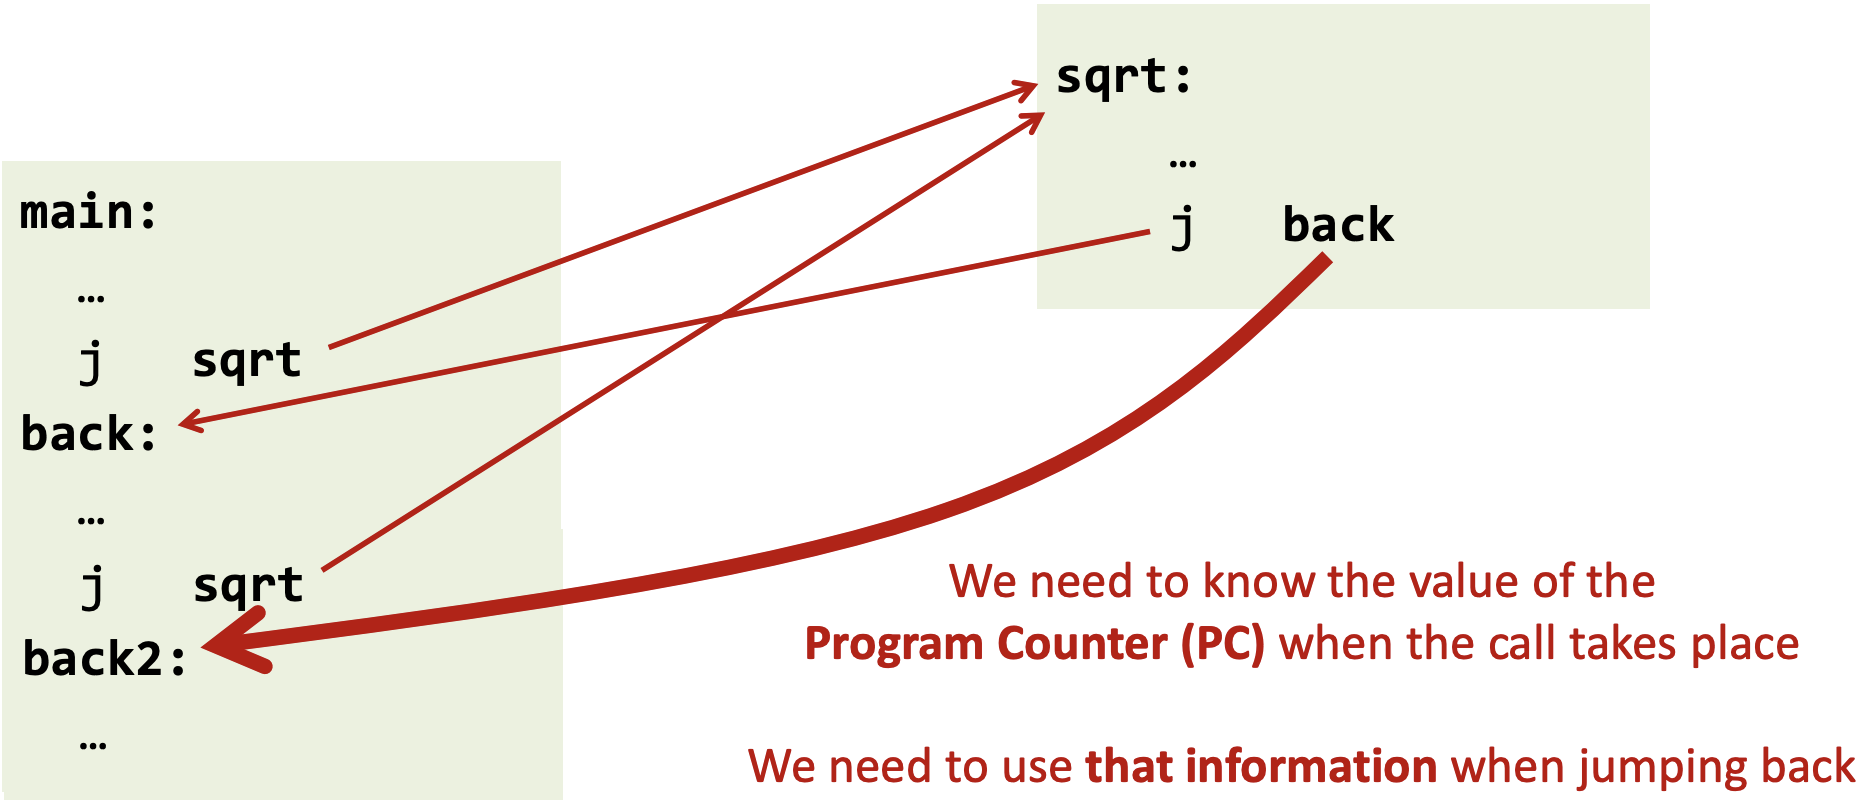
\includegraphics[width=0.75\textwidth]{chapters/chapter1b/images/function.png}
\end{center}
\textit{With this approach the function doesn't know where to return to after being called (back2 or back)}
\textbf{For the next part, remember, the Program Counter is distinct from general-purpose registers. It is dedicated to managing the flow of instruction execution, while general registers are used for data manipulation. }
\subsubsection{The Good Approach}
\textit{The right approach involves using the Jump and Link instruction \texttt{jal}, here loading PC + 4 (remember 4 bytes per Instruction) into x1 as a way to come back from the function.} \\
\begin{minipage}[htp]{0.4\textwidth}
\begin{assembly}
main:
    ...
    jal x1, sqrt
    ...
    ...
    jal x1, sqrt
\end{assembly}    
\end{minipage}
\hfill
\vline
\hfill
\begin{minipage}[htp]{0.4\textwidth}
\begin{assembly}
sqrt:
    ...
    ...
    jr x1
\end{assembly}
\end{minipage} \\
\textit{Both times x1 was used to store the return adress, and there is a reason for that (Register Conventions Sections).}

\subsection{Jump Instructions}
\textit{There are only two core real jump instructions in RISCV, \texttt{jal} (jump and link) and \texttt{jalr} (jump and link register), the rest are pseudo instructions using them.} \\

\begin{center}
    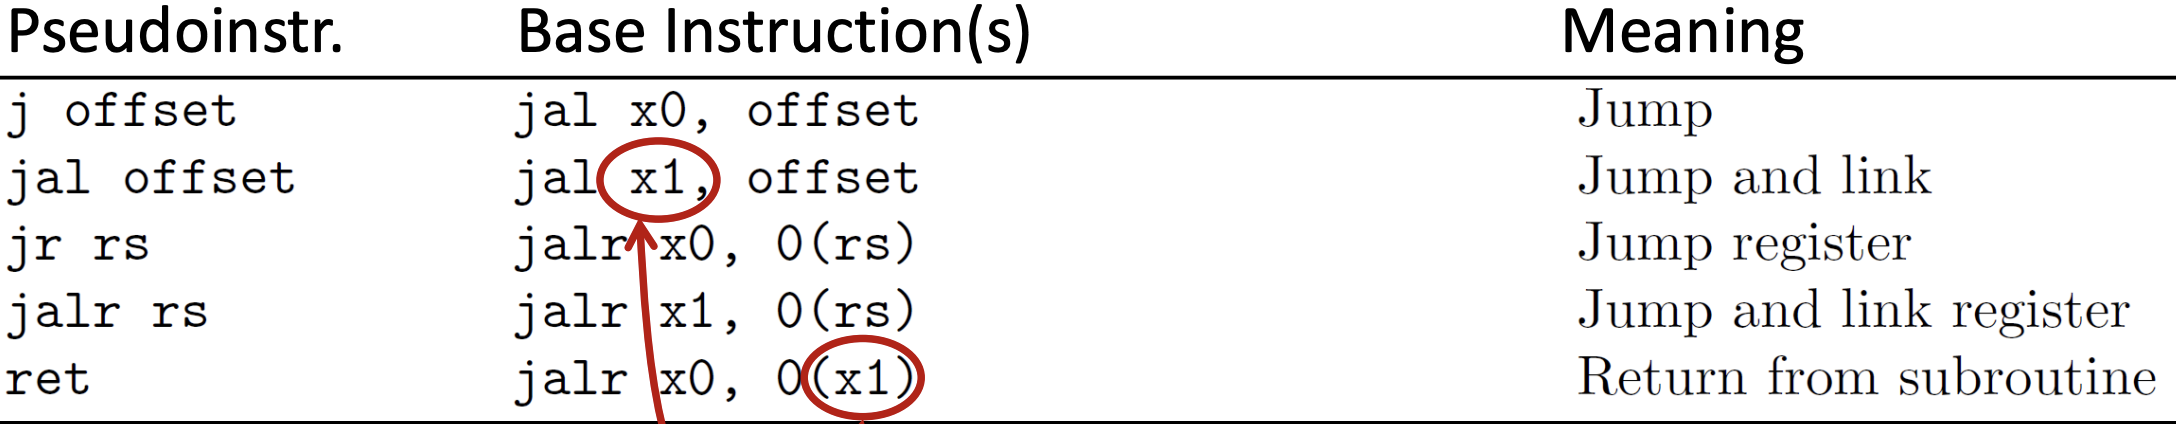
\includegraphics[width=0.75\textwidth]{chapters/chapter1b/images/jump.png}
\end{center}
\newpage
\subsection{Register Conventions}
\textit{Register conventions are rules that dictate how registers are used in a program, here are the ones we've seen for now} \\
\begin{center}
    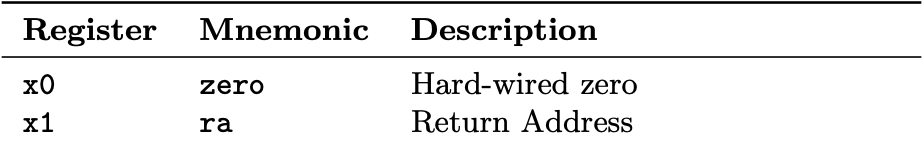
\includegraphics[width=0.75\textwidth]{chapters/chapter1b/images/conventions.png}
\end{center}

\subsection{Back to the good (not so good) approach}
\textit{There's still a problem with the previous approach, say for example you want to call a function from another function.}
\begin{center}
    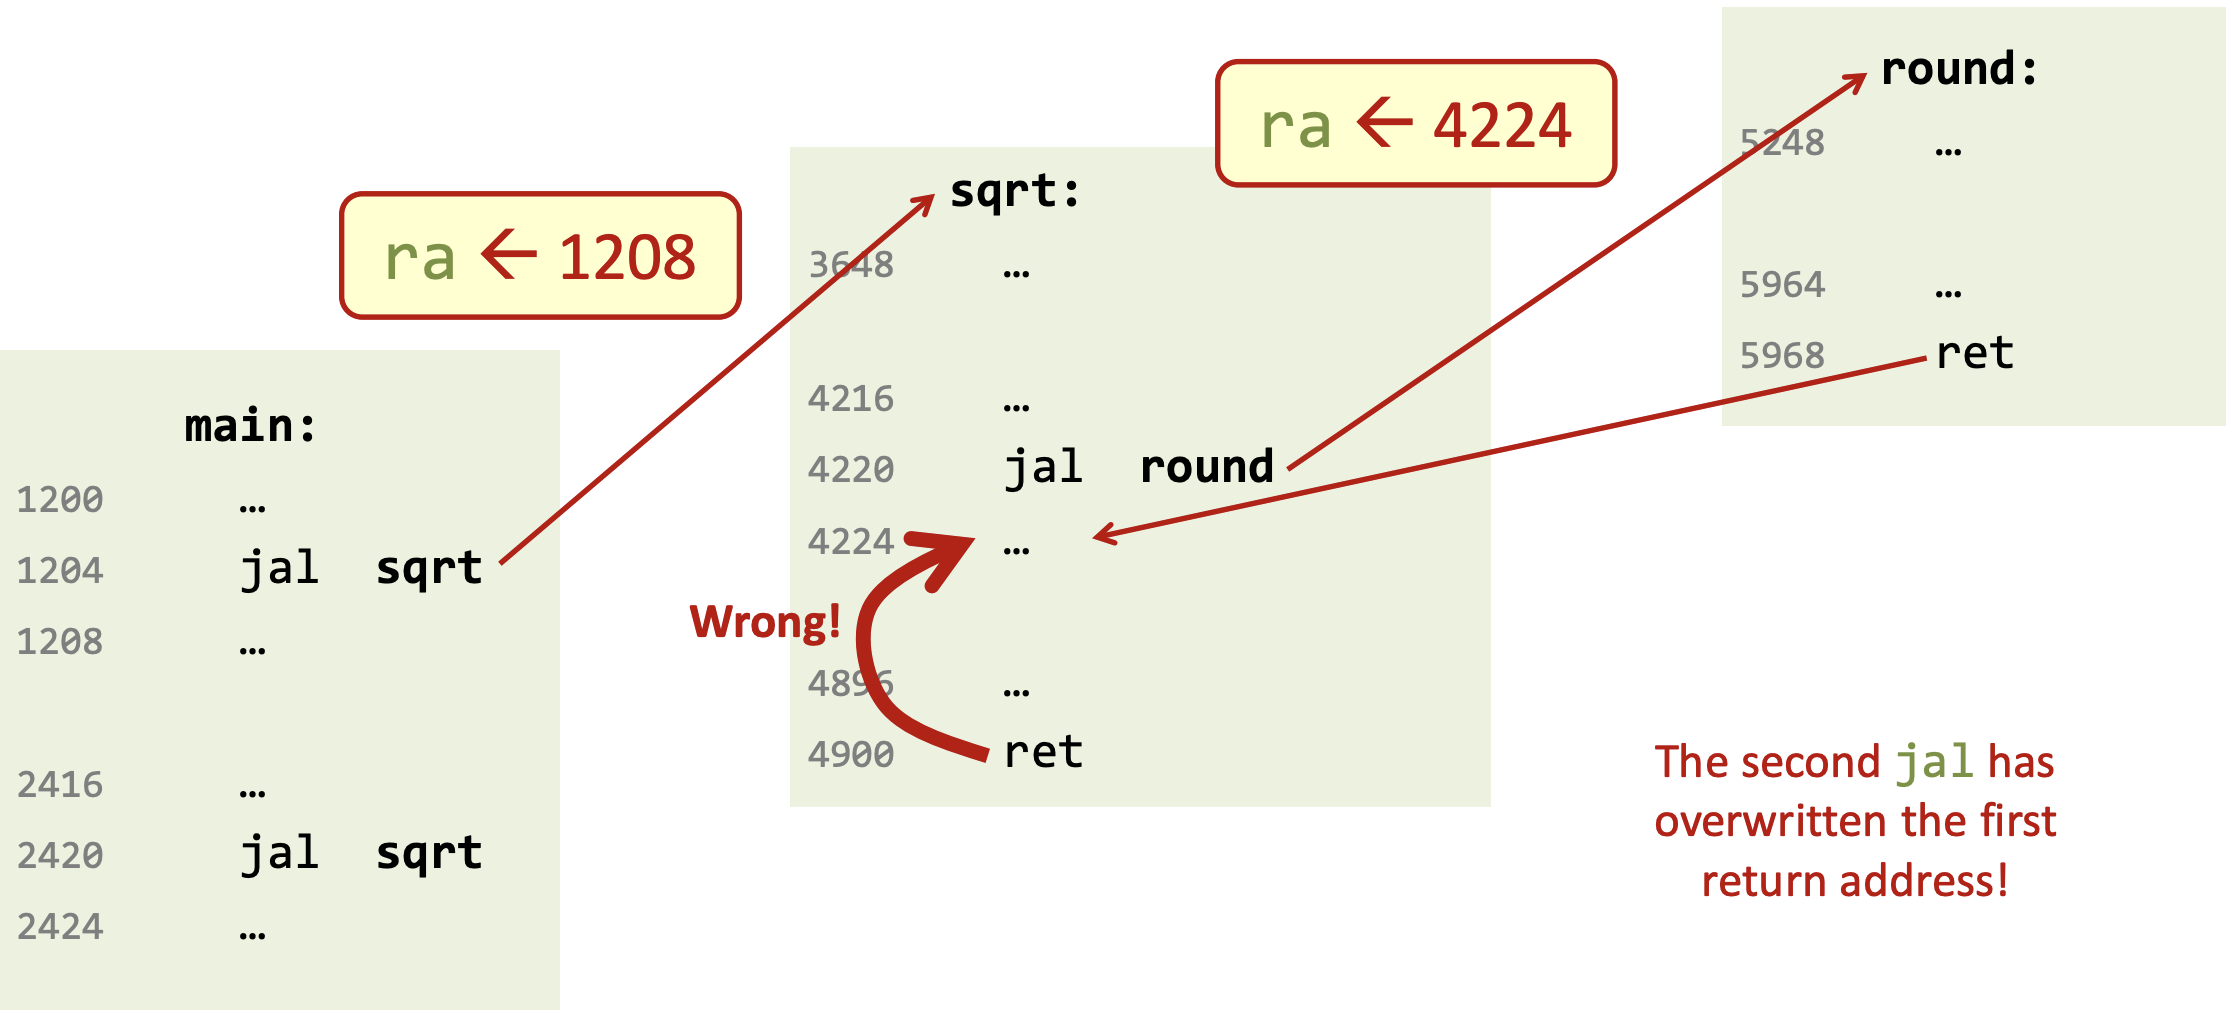
\includegraphics[width=0.75\textwidth]{chapters/chapter1b/images/function2.png}
\end{center}
\textbf{Here the allocated space for the return address is overwritten by the second function call, and the first function can't return to the right place.}
\subsection{One simple solution (still not good)}
\textit{One solution would be to say that a range of registers are used for certain functions and that they can't be used by other functions.}
\begin{center}
    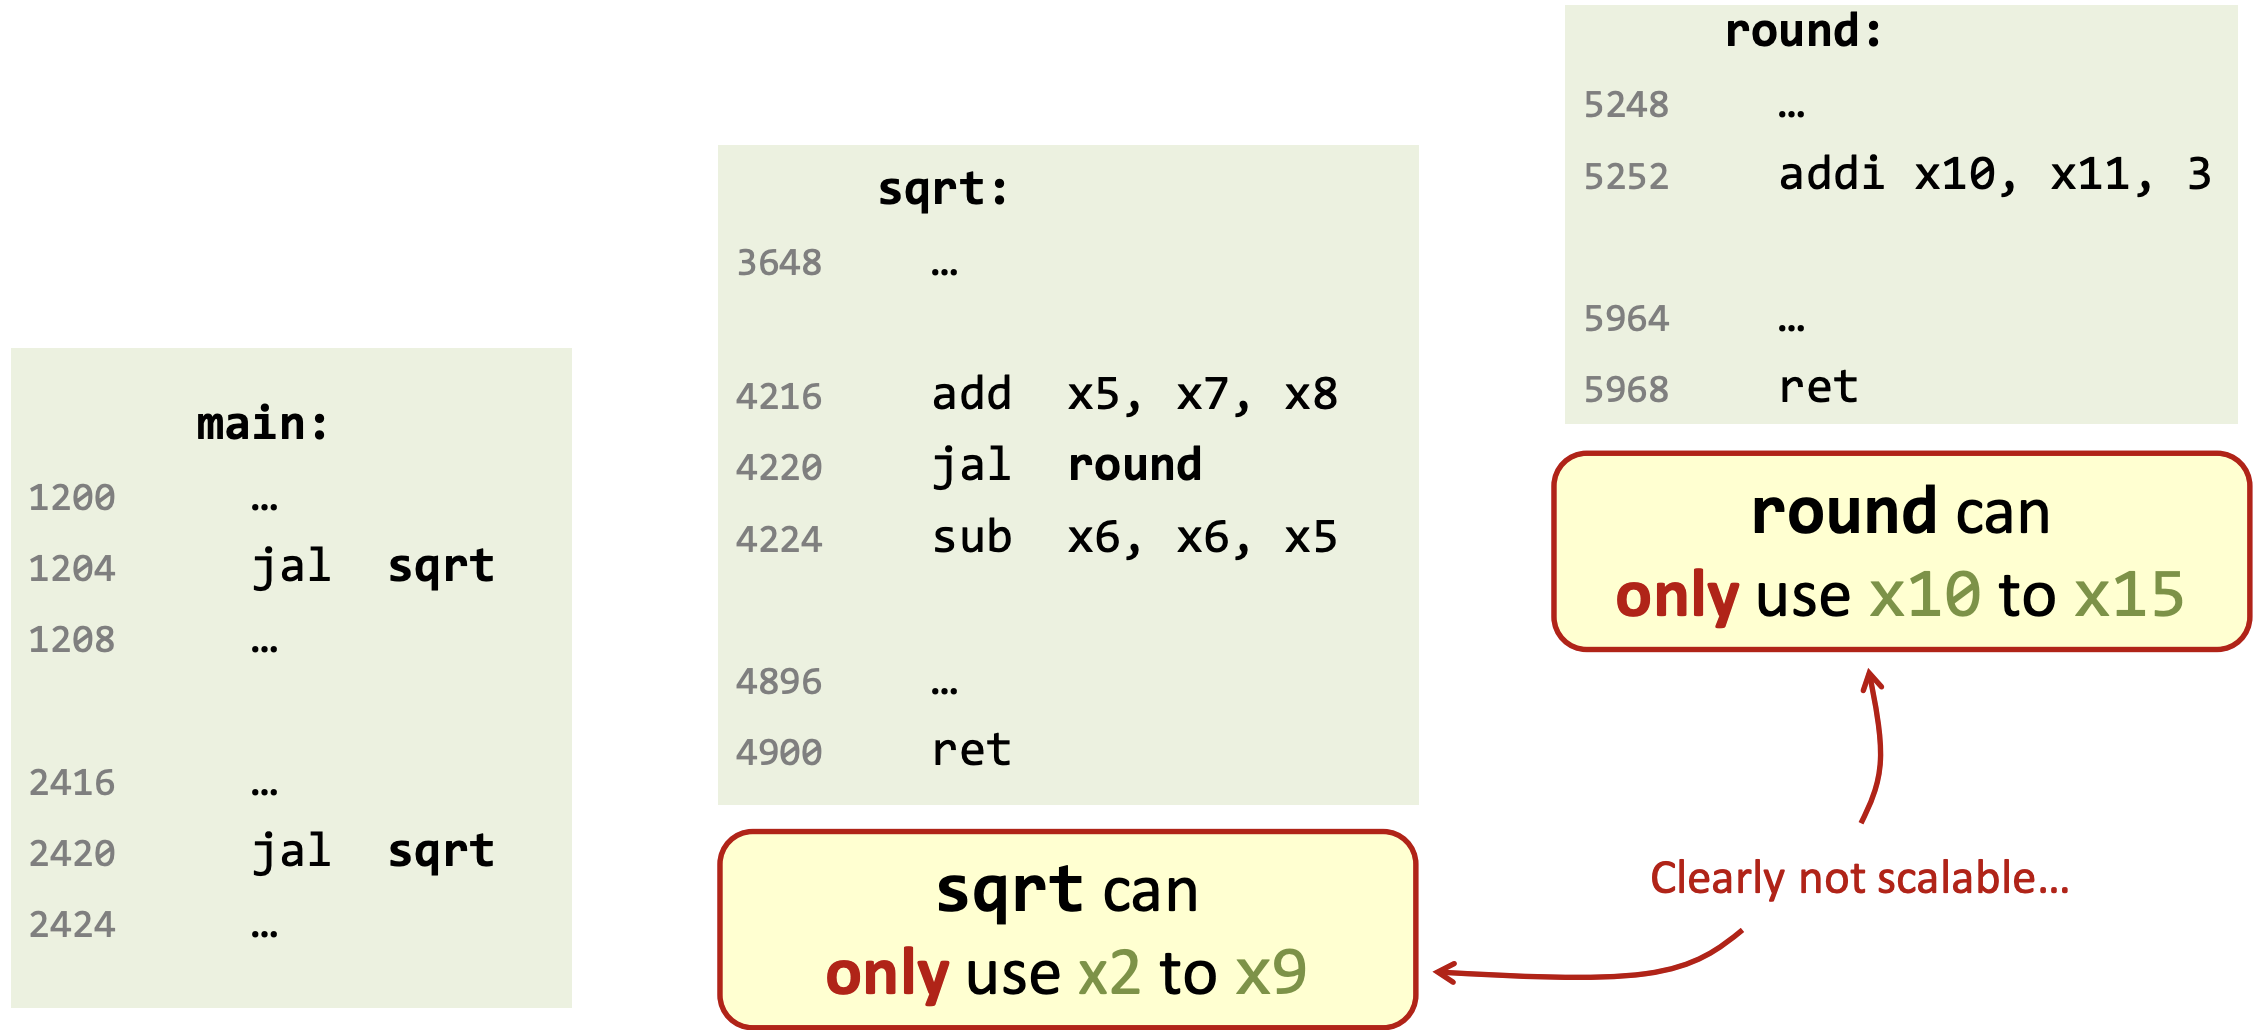
\includegraphics[width=0.75\textwidth]{chapters/chapter1b/images/function3.png}
\end{center}
\textbf{The problem here is that it's still not very scalable.}
\subsection{Acquire storage resources the function needs (still not it)}
One simple solution to our problem would be to allocate memory for the function at in the data section of the program. \\
\begin{minipage}[htp]{0.4\textwidth}
\begin{assembly}
.data
sqrt_save_ra: .word 0
sqrt_save_x5: .word 0 
\end{assembly}
\end{minipage}
\hfill
\vline
\hfill
\begin{minipage}[htp]{0.4\textwidth}
\begin{assembly}
.text
sqrt:
...
add x5, x7, x8
sw ra, sqrt_save_ra
sw x5, sqrt_save_x5
jal round
lw ra, sqrt_save_ra
lw x5, sqrt_save_x5
sub x6, x6, x5
...
ret
\end{assembly}
\end{minipage}
\subsubsection{Problem: Recursive Functions}
\textit{The problem here is that the return address is overwritten by the recursive call.}
\begin{center}
\begin{assembly}
.data
    find_child_save_ra: .word 0
.text
    find_child:
    ...
    sw ra, find_child_save_ra
    jal find_child
    lw ra, find_child_save_ra
    ...
    ret
\end{assembly}
\end{center}
\subsection{The Stack}
\textit{The Solution to our Problem is this, the Stack.} \\
\textbf{The Stack is a region of memory that grows and shrinks as needed.} \\
We may use a register (e.g \texttt{x2}) to point to the first used word after the end of the used region.
\begin{center}
    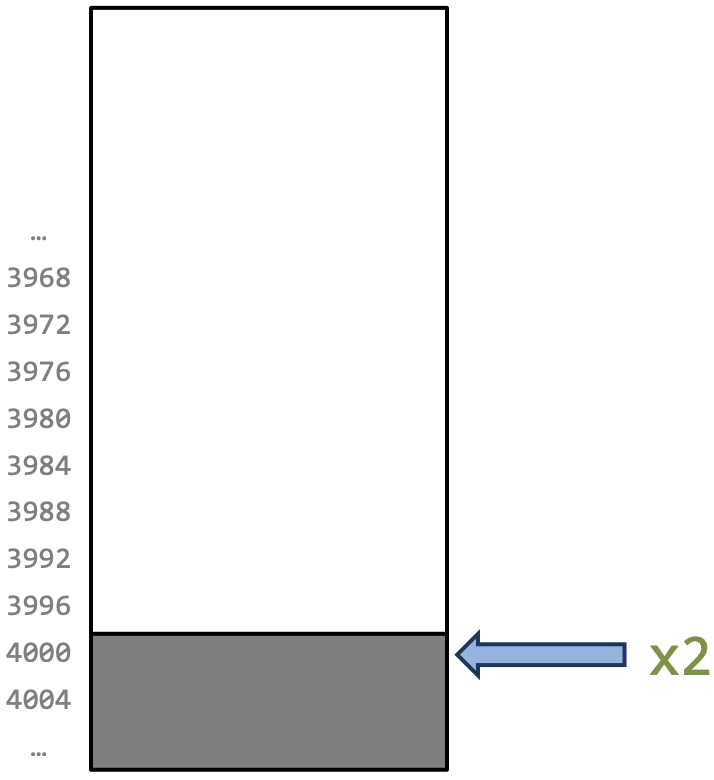
\includegraphics[width=0.4\textwidth]{chapters/chapter1b/images/stack.png}
\end{center}

\subsubsection{Dynamic Memory Allocation}
The Stack, contrary to the Data Section, is dynamic and can be used to allocate memory when needed. This means that during program execution, variables or temporary data can be stored in the stack, which grows or shrinks depending on the operations performed. \\
 The \texttt{stack pointer}, typically register x2, is used to manage the allocation and deallocation of memory.

\begin{minipage}[htp]{0.4\textwidth}
\textit{In this instruction, for example, we allocate 12 bytes in the stack. We achieve this by decrementing the stack pointer (x2) by 12. This ensures that the new memory space is available for temporary storage.}
\begin{assembly}
addi x2, x2, -12
\end{assembly}
\end{minipage}
\hfill
\vline
\hfill
\begin{minipage}[htp]{0.4\textwidth}
\begin{center}
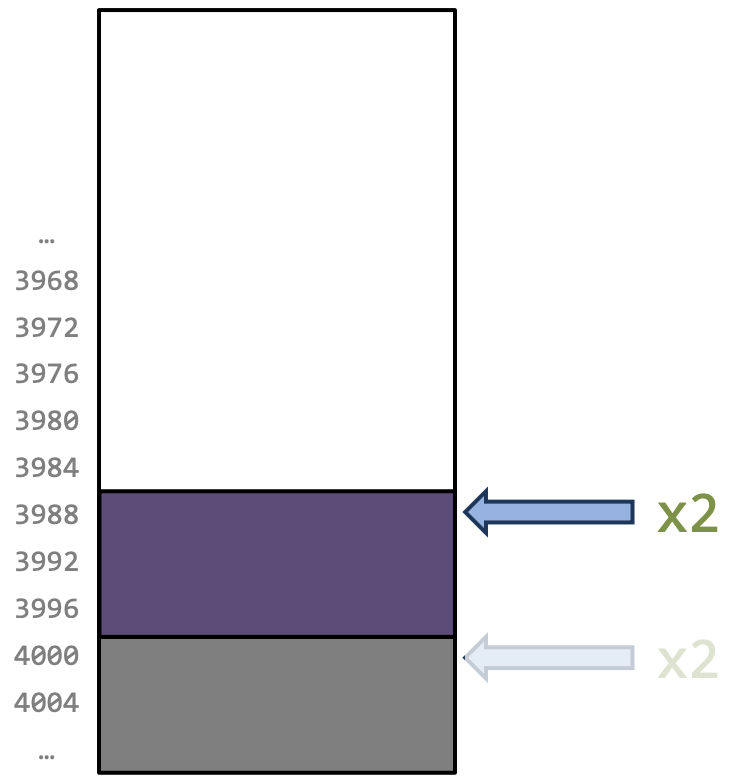
\includegraphics[width=0.75\textwidth]{chapters/chapter1b/images/stack2.png}
\end{center}
\end{minipage}

\subsubsection{Retrieving Data from the Stack}
Once memory has been allocated on the stack, we can store or retrieve data from it. In this case, we are retrieving data that was previously saved in the stack. The lw (load word) instruction is used to load the values stored at different offsets in the stack.

\begin{minipage}[htp]{0.4\textwidth}
\textit{In this case, we retrieve three different values from the stack using the lw instruction, which loads a 4-byte value into the specified registers (ra, x5, and x6). The offsets (0, 4, and 8) refer to different positions in the 12 bytes we allocated earlier.}
\begin{assembly}
lw ra, 0(x2)
lw x5, 4(x2)
lw x6, 8(x2)
\end{assembly}
\end{minipage}
\hfill
\vline
\hfill
\begin{minipage}[htp]{0.4\textwidth}
\begin{center}
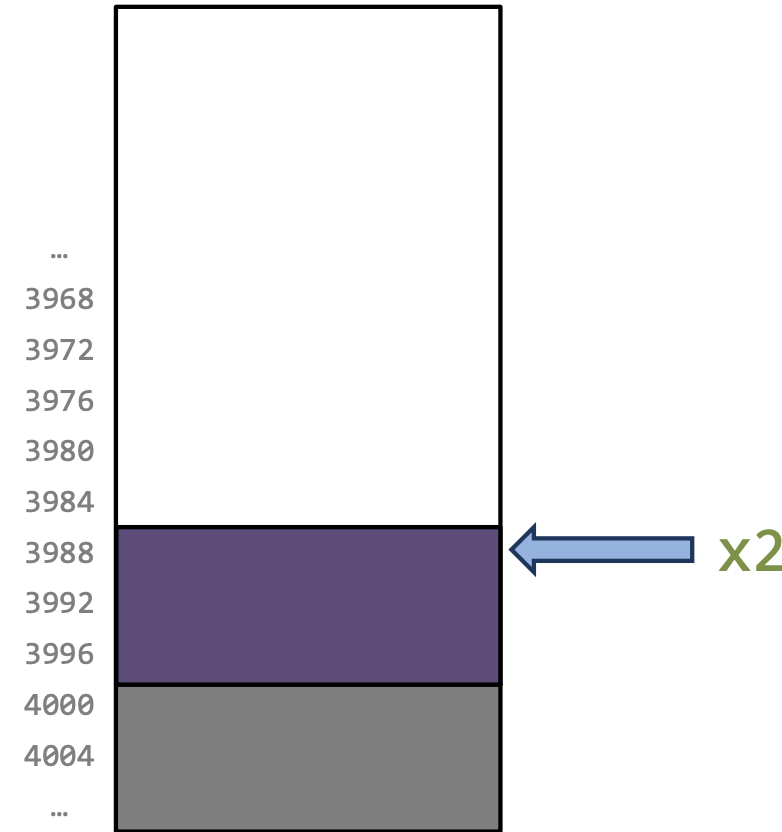
\includegraphics[width=0.75\textwidth]{chapters/chapter1b/images/stack3.png}
\end{center}
\end{minipage}
\newpage

\subsubsection{Memory Deallocation}
After the data has been used or is no longer needed, it is good practice to deallocate the memory to ensure proper management of the stack. We deallocate memory by adjusting the stack pointer (x2) back to its original position.

\begin{minipage}[htp]{0.4\textwidth}
\textit{In this instruction, we restore the stack to its previous state by adding 12 back to the stack pointer (x2).} \\ \textit{This effectively "frees" the 12 bytes of memory we had allocated earlier.}
\begin{assembly}
addi x2, x2, 12
\end{assembly}
\end{minipage}
\hfill
\vline
\hfill
\begin{minipage}[htp]{0.4\textwidth}
\begin{center}
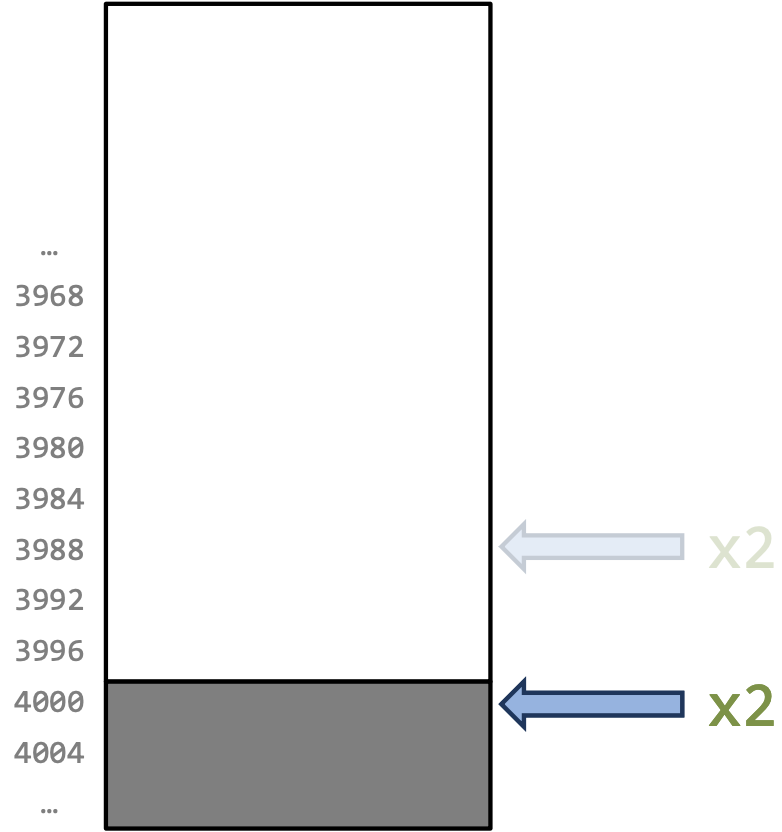
\includegraphics[width=0.75\textwidth]{chapters/chapter1b/images/stack4.png}
\end{center}
\end{minipage}

\subsubsection{The Stack Pointer}
\textit{The Stack Pointer is a register that points to the top of the stack, by convention it corresponds to the x2 register} \\
\begin{center}
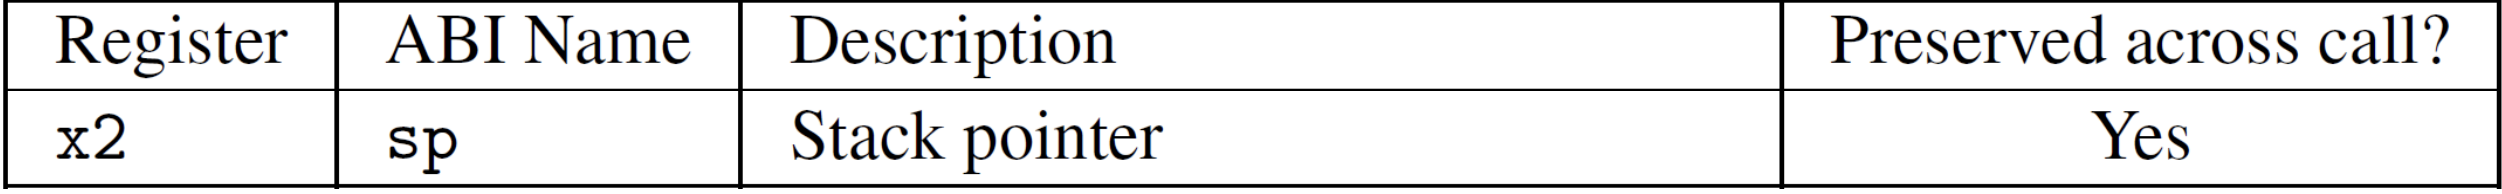
\includegraphics[width=0.75\textwidth]{chapters/chapter1b/images/conventions2.png}
\end{center}
\small
\textit{Other architectures have special instructions to place stuff on
the stack (push) and to retrieve it (pop)} \\
\vspace*{10px}
\begin{minipage}[htp]{0.4\textwidth}
\begin{lstlisting}
PUSH AX
\end{lstlisting}
\end{minipage}
\hfill
\vline
\hfill
\begin{minipage}[htp]{0.4\textwidth}
\begin{assembly}
add sp, sp, -4
sw x5, 0(sp)
\end{assembly}
\end{minipage}

\subsection{Spilling Registers to Memory}
\textit{Spilling registers to memory involves saving register values to the stack when more registers are needed or to prevent overwriting important data, allowing the registers to be reused. This technique is also used in function calls to save the return address, ensuring the program can correctly return control after the function finishes.}
\begin{center}
    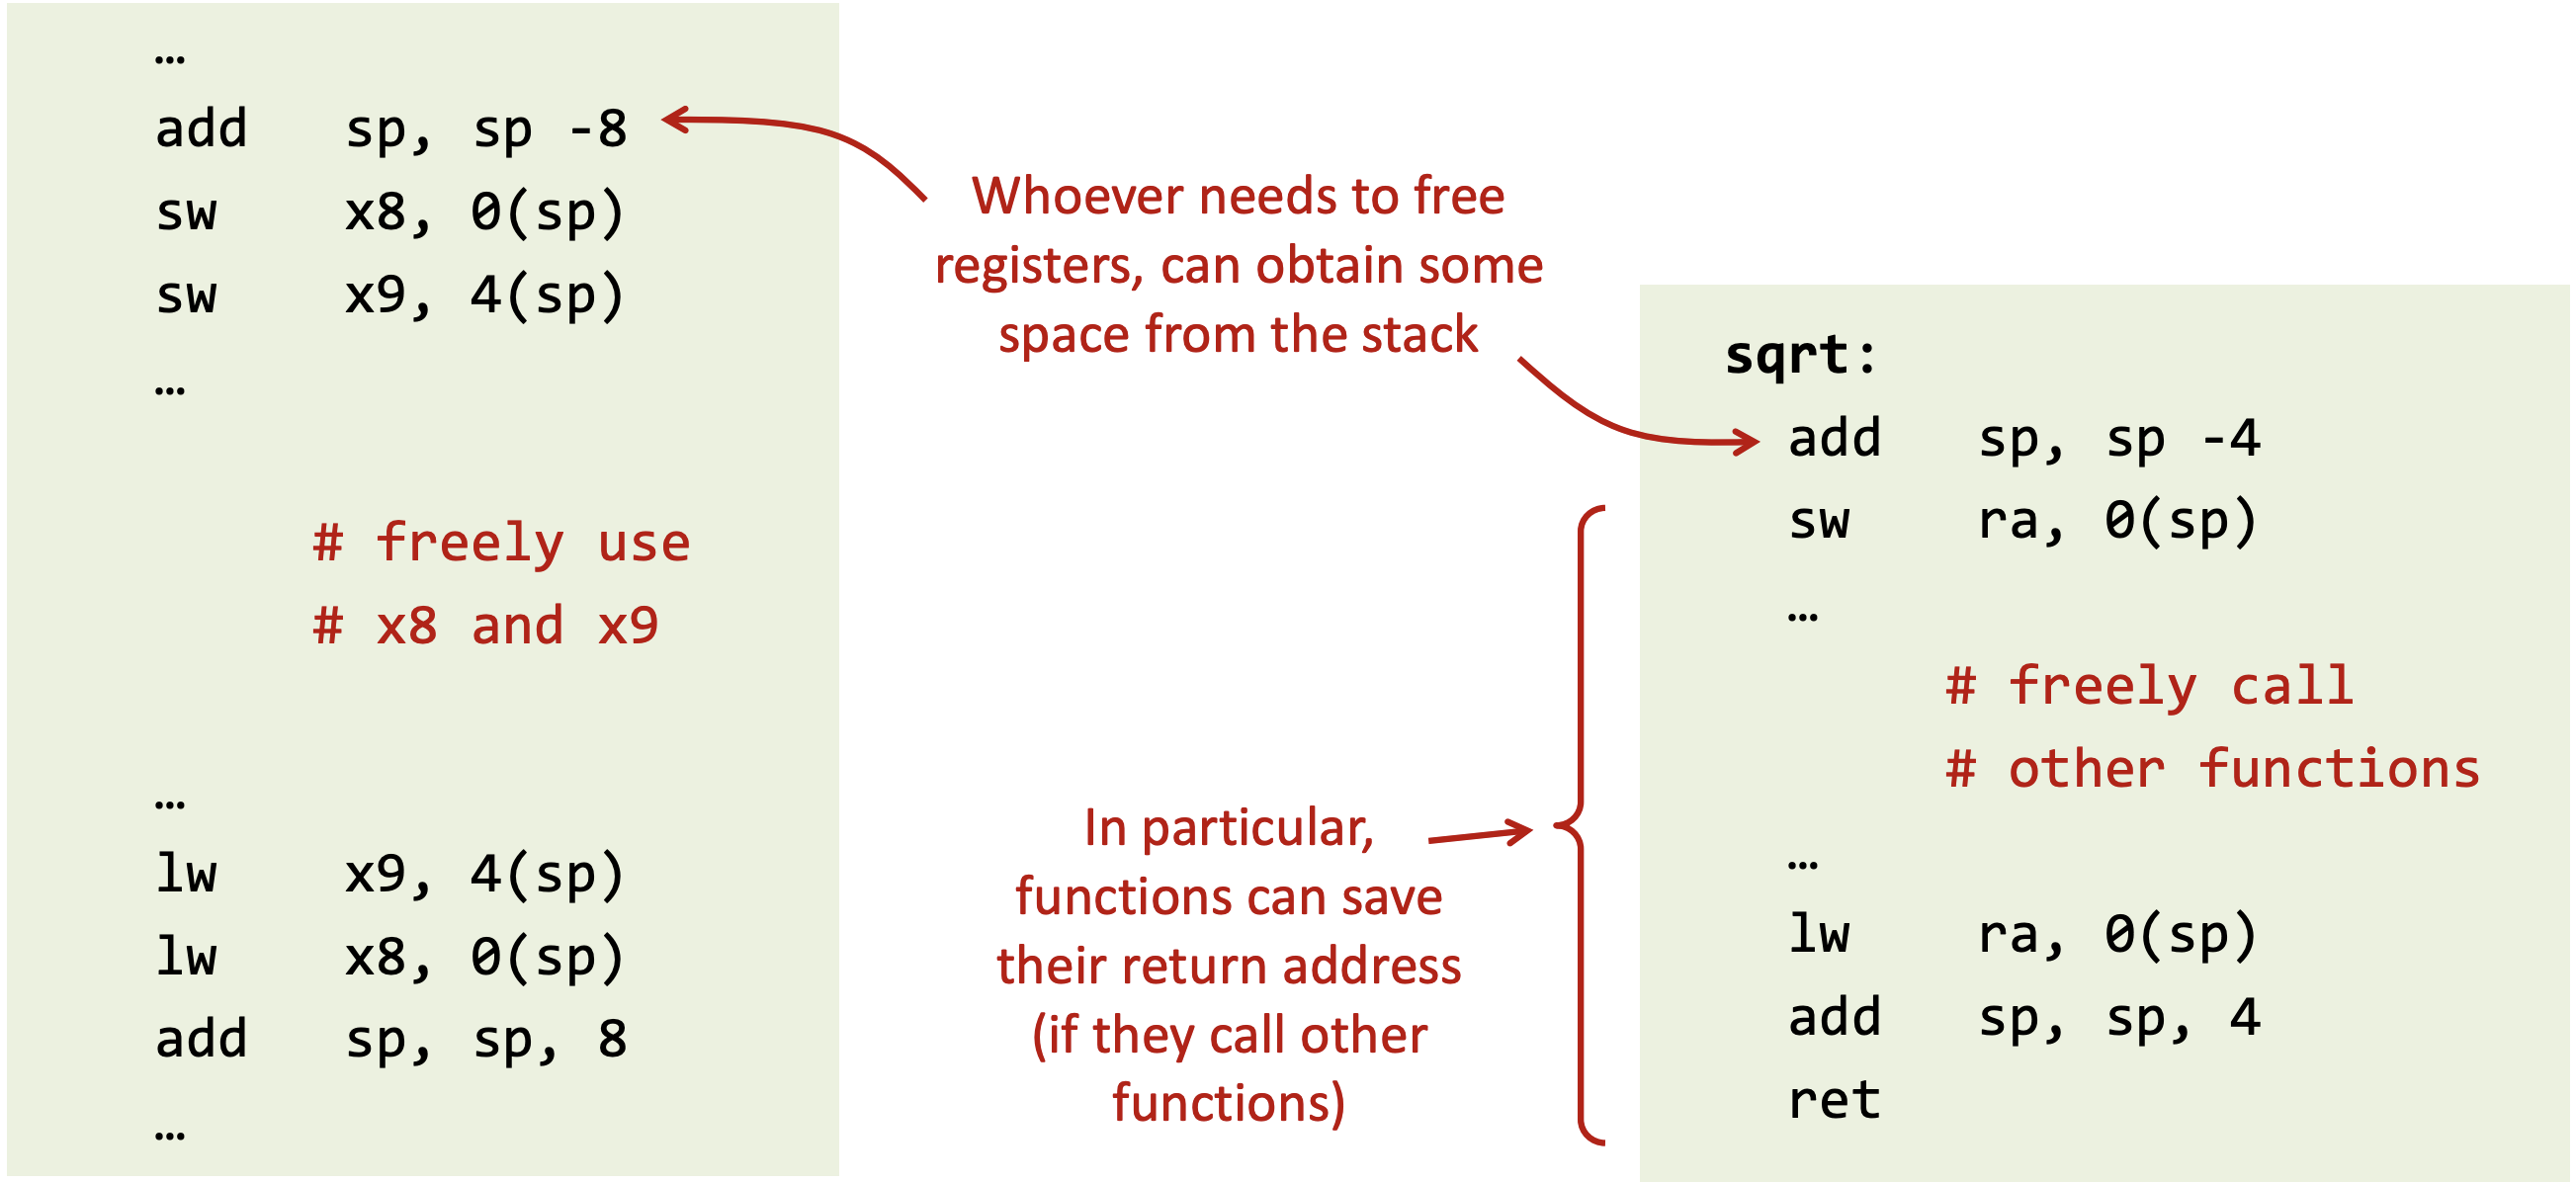
\includegraphics[width=0.75\textwidth]{chapters/chapter1b/images/spilling.png}
\end{center}

\subsection{Register across functions}
In assembly programming, handling registers across functions can be managed in two main ways: either functions \textbf{change registers} and expect the caller to save their values, or functions \textbf{preserve registers} and ensure that the register values remain the same across function calls.

\begin{itemize}
    \item On the left, the function \texttt{sqrt} changes the value of register \texttt{x20}, requiring the caller to save and restore its value.
    \item On the right, the function \texttt{sqrt} preserves the value of \texttt{x20}, ensuring that the caller does not need to manage the saving and restoring.
\end{itemize}

This distinction is important, but it does not cause issues as long as there is agreement on how registers are handled. \\
\textit{In case it's still not clear, we're looking at the \texttt{sw} instruction}

\begin{center}
    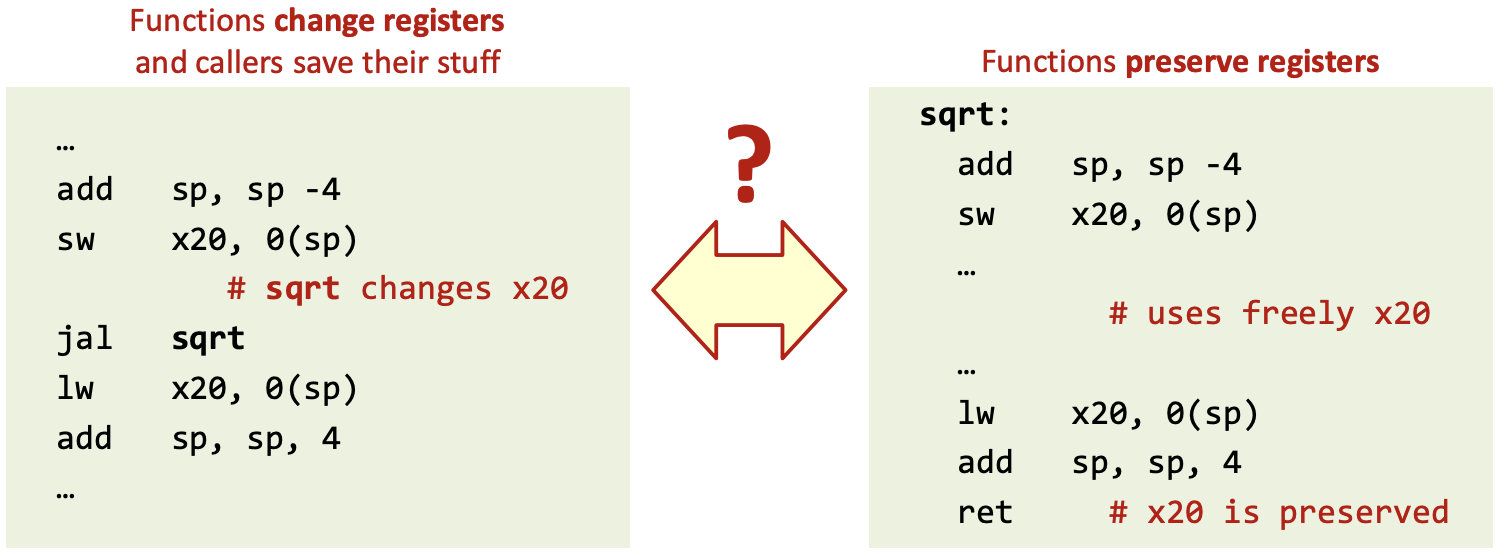
\includegraphics[width=0.7\textwidth]{chapters/chapter1b/images/registers.png}
\end{center}

\subsection{Preserving Registers}
In RISC-V, register preservation is managed through a combination of callee-saved and caller-saved registers. \\
Callee-saved registers (such as \texttt{s0}, \texttt{s1}, and \texttt{s2-11}) are preserved by the called function, ensuring that their values remain unchanged after the function call.  \\
Caller-saved registers (such as \texttt{t0}, \texttt{t1-2}, and \texttt{t3-6}) are temporary and do not need to be preserved by the called function, meaning the caller must save them if their values are important. \\
\begin{center}
    \begin{tabular}{|c|c|c|c|}
        \hline
        \textbf{Register} & \textbf{ABI Name} & \textbf{Description} & \textbf{Preserved across call?} \\ \hline
        x0  & zero  & Hard-wired zero                        & \textemdash    \\ \hline
        x1  & ra    & Return address                         & No             \\ \hline
        x2  & sp    & Stack pointer                          & Yes            \\ \hline
        x5  & t0    & Temporary/alternate link register      & No             \\ \hline
        x6--7 & t1--2 & Temporaries                          & No             \\ \hline
        x8  & s0/fp & Saved register/frame pointer           & Yes            \\ \hline
        x9  & s1    & Saved register                        & Yes            \\ \hline
        x18--27 & s2--11 & Saved registers                   & Yes            \\ \hline
        x28--31 & t3--6 & Temporaries                        & No             \\ \hline
        \end{tabular}
\end{center}

\section{Passing Arguments in RISC-V}

In RISC-V, there are two main ways to pass arguments to functions:

\subsection{Option 1: Using Registers}
- Specific registers are used to pass arguments and return results. \\
\vskip 0.1in
- This can be done in a straightforward way, where each function uses different registers (e.g., passing an argument in \texttt{x5} and returning the result in \texttt{x6}).
\vskip 0.1in
- A more structured approach is to follow a convention where arguments are passed in registers \texttt{x10} to \texttt{x17}, with results returned in \texttt{x10}.  \\
\vskip 0.1in
- The limitation: if there are more arguments than available registers (e.g., more than 8 arguments), this approach is insufficient.  \\

\subsection{Option 2: Using the Stack}
- When registers are not enough, extra arguments are placed on the stack.  \\
\vskip 0.1in
- The stack offers a universal solution because it has no practical limit on size.  \\
\vskip 0.1in
- However, using the stack is more complex and requires additional work compared to using registers.  \\

\subsection{The RISC-V Approach}
- RISC-V uses a combination of both methods.  \\
\vskip 0.1in
- Registers \texttt{x10} to \texttt{x17} are used to pass arguments, with \texttt{x10} and \texttt{x11} also handling return values. \\
\vskip 0.1in
- If more arguments are needed beyond what these registers can handle, they are passed via the stack. 

\begin{center}
    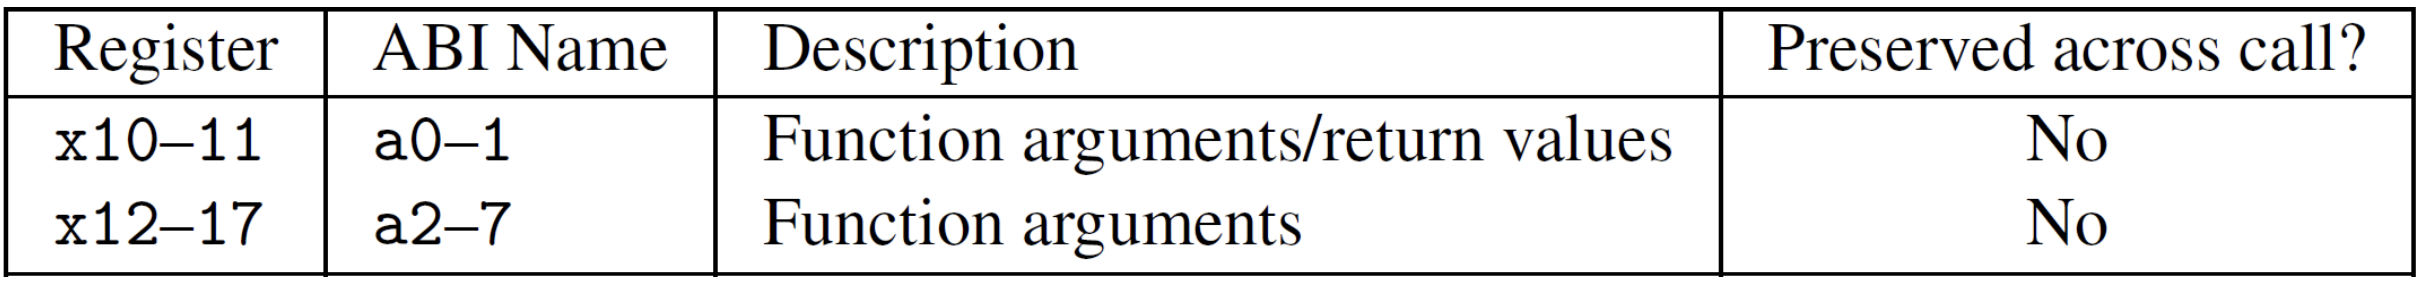
\includegraphics[width=0.75\textwidth]{chapters/chapter1b/images/arguments.png}
\end{center}
\textit{Register reserved for arguments and return values in RISC-V.}

\section{Summary of RISC-V Register Conventions}
\begin{center}
    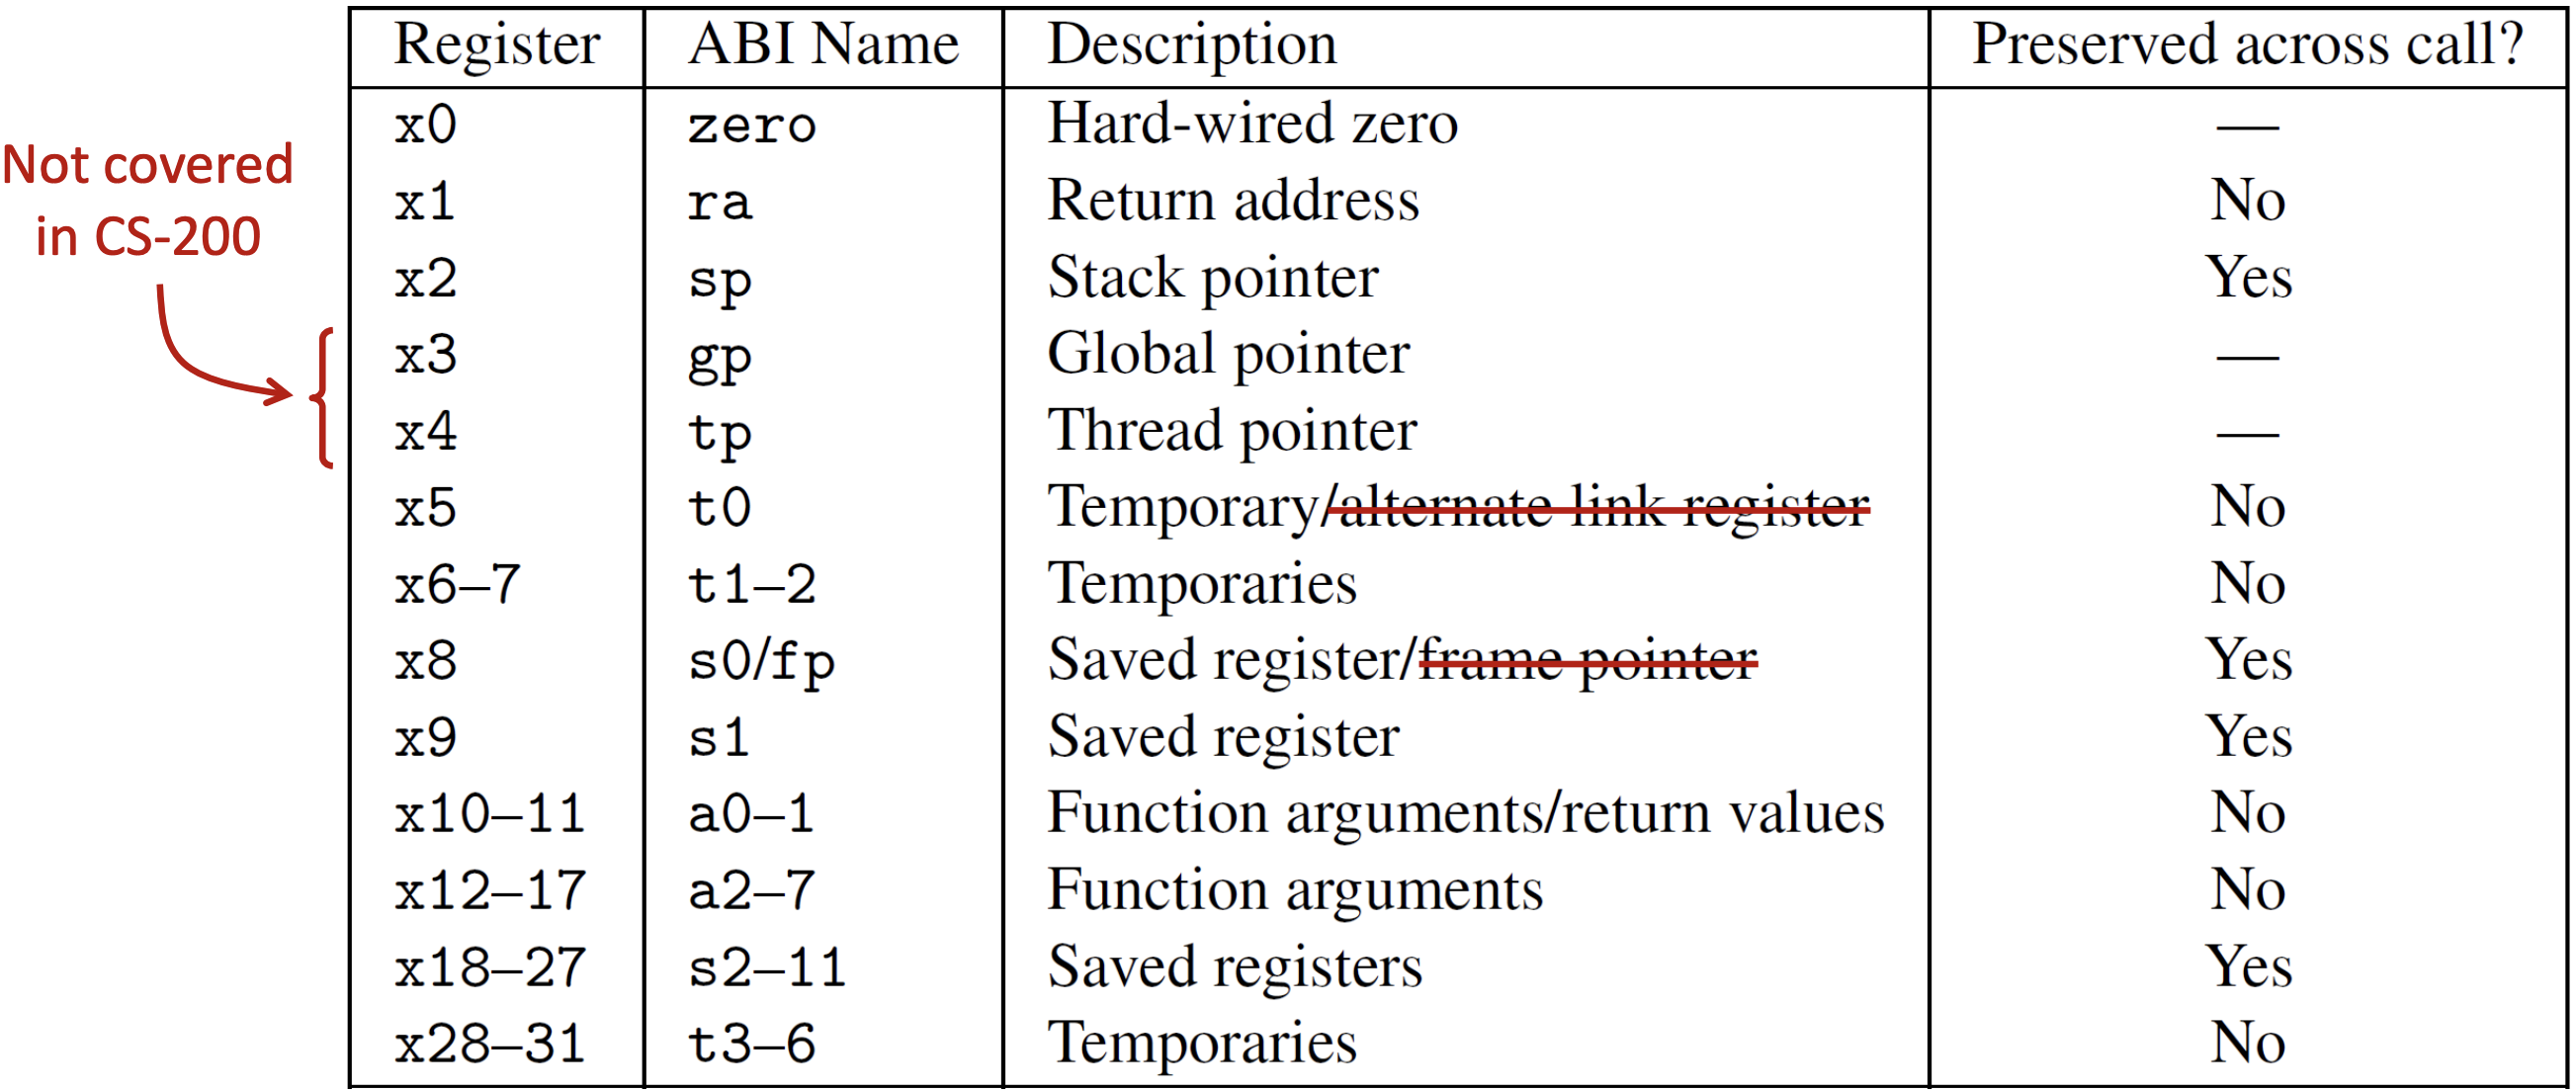
\includegraphics[width=0.75\textwidth]{chapters/chapter1b/images/summary.png}
\end{center} % Including chapter0.tex from chapters folder
\chapter{Part I(c) - ISA Memory and Addressing Modes - W 2.1}

\section{Memory}
\textit{Memory is a really important component of a computing system, we store our programs in it, we store our data in it, and it's through memory that we receive and send data.} \\ \vspace*{5px}
\textbf{Though memory is very useful it has three main drawbacks:} \\ \vspace*{5px}
\begin{itemize}
    \item[-] It's \textbf{slow} $\rightarrow$ Caches 
    \item[-] It's \textbf{finite} $\rightarrow$ Virtual Memory
    \item[-] It can make an ISA \textbf{too complex} $\rightarrow$ Pipelining
\end{itemize}
\textit{no worries we'll cover each one of these in this chapter.}

\subsection{Address and Data}
\textit{Data in Memory can be accessed by an adress, meaning i's a \textit{Random Access} (it can access a memory value without going through the preceding ones).} \\ \vspace*{5px}
\textit{Professor Remark: "There's not anything random about this memory, we'd better call it and abitrary access memory. (!not and official  name)"} \\ \vspace*{5px}
\vspace*{5px}
\begin{minipage}[htp]{0.45\textwidth}
\begin{center}
    \begin{tabular}{|c|c|}
    \hline
    \textbf{Address} & \textbf{Value} \\
    \hline
    \texttt{0} & 12 \\ 
    \hline
    \texttt{1} & 6 \\ 
    \hline
    \texttt{2} & 4 \\ 
    \hline
    \texttt{3} & 1 \\ 
    \hline
    \texttt{4} & 0 \\ 
    \hline
    \texttt{5} & 3 \\ 
    \hline
    \texttt{6} & 1 \\ 
    \hline
    \texttt{7} & 13 \\ 
    \hline
    \texttt{8} & 15 \\ 
    \hline
    \texttt{9} & 9 \\ 
    \hline
    \texttt{10} & 3 \\ 
    \hline
    \texttt{11} & 5 \\ 
    \hline
    \texttt{12} & 0 \\ 
    \hline
    \texttt{13} & 0 \\ 
    \hline
    \texttt{14} & 0 \\ 
    \hline
    \texttt{15} & 0 \\ 
    \hline
    \end{tabular}
\end{center}
\end{minipage}
\hfill
\vline
\hfill
\begin{minipage}[htp]{0.45\textwidth}
\begin{center}
    \begin{tabular}{|c|c|}
    \hline
    \textbf{Write} & \textbf{Read} \\ 
    \hline
    \texttt{\textbf{Memory[5] = 3}} & \texttt{Memory[5]?} \\ 
    \hline
    \end{tabular}
\end{center}
\end{minipage}

\section{Many Types of Memories}
We may distinguish between different types of memories based on their \textbf{technology}, such as SRAM, DRAM, EPROM, and Flash, and their \textbf{capabilities}, including \textbf{speed}, \textbf{capacity}, \textbf{density}, \textbf{writability} (whether they are writable, permanent, or reprogrammable), as well as their \textbf{size}, \textbf{volatility}, and \textbf{cost}. \\ \vspace*{5px}
\subsection{Functional Taxonomy of Memories}
\begin{center} 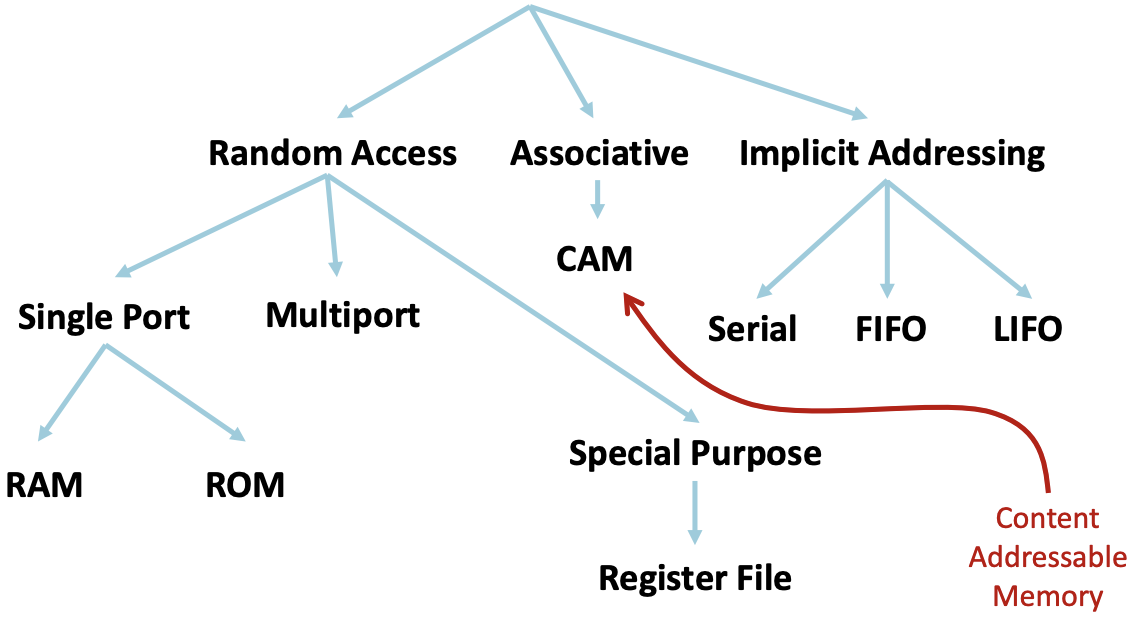
\includegraphics[width=0.45\textwidth]{chapters/chapter1c/images/funct_tax.png} \end{center}
\begin{itemize}
    \item[] \textbf{Multiport} memory allows simultaneous access by multiple processors, while \textbf{single-port} memory supports only one at a time.
    \item[] \textbf{Non-Random Access memories}
    \begin{itemize}
        \item \textbf{Adsociative} memories enable fast data retrieval by content rather than address, making it useful for cache memory, pattern recognition, and efficient lookups in large datasets.
        \item In \textbf{Implicit addressing} the address of the data to be operated on is inferred directly by the operation code (opcode), without explicitly specifying the address in the instruction.
    \end{itemize}
\end{itemize}


\subsection{Taxonomy of Random Access Memories}
\begin{center}
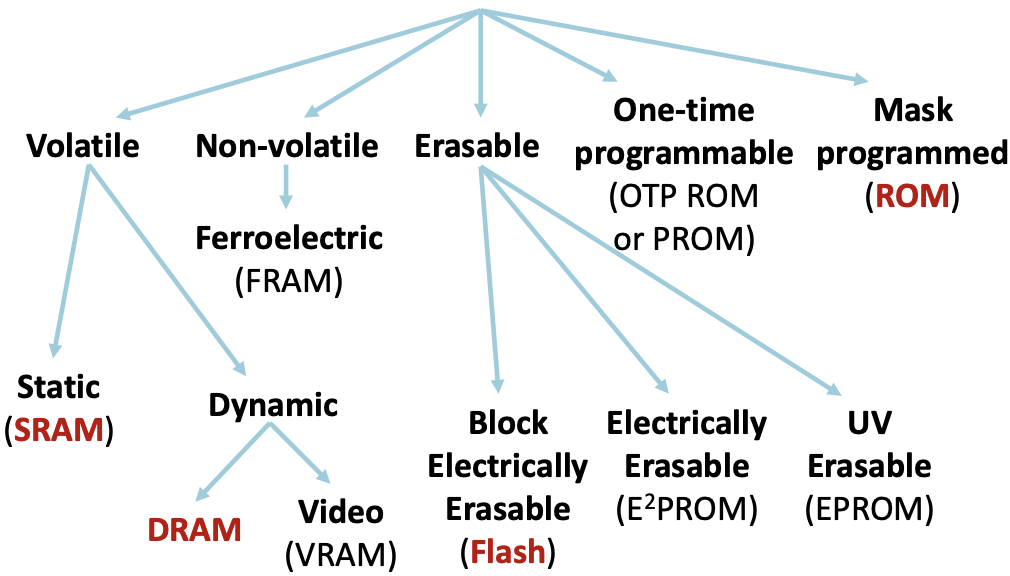
\includegraphics[width=0.45\textwidth]{chapters/chapter1c/images/ram_tax.png}
\end{center}
\newpage
\subsection{Basic Structure}
\textit{Remember, a Data Flip Flop, stores a 1 bit value by updating the output value to the input value at the rising edge of the clock signal.} \\ \vspace*{5px}
\begin{minipage}[htp]{0.35\textwidth} 
\begin{center}
    \begin{tabular}{|c|c|}
        \hline
        \textbf{Address} & \textbf{Value} \\ 
        \hline
        \texttt{0} & 12 \\ 
        \hline
        \texttt{1} & 6 \\ 
        \hline
        \texttt{2} & 4 \\ 
        \hline
        \texttt{3} & 1 \\ 
        \hline
        \texttt{4} & 0 \\ 
        \hline
        \texttt{5} & 3 \\ 
        \hline
        \texttt{6} & 1 \\ 
        \hline
        \texttt{7} & 13 \\ 
        \hline
        \texttt{8} & 15 \\ 
        \hline
        \texttt{9} & 9 \\ 
        \hline
        \texttt{10} & 3 \\ 
        \hline
        \texttt{11} & 5 \\ 
        \hline
        \texttt{12} & 0 \\ 
        \hline
        \texttt{13} & 0 \\ 
        \hline
        \texttt{14} & 0 \\ 
        \hline
        \texttt{15} & 0 \\ 
        \hline
        \end{tabular}
\end{center}
\end{minipage}
\hfill
\vline
\hfill
\begin{minipage}[htp]{0.35\textwidth}
\textbf{16 x 4 Memory Cells (~Special DFFs (Data Flip-Flops))} \\
\begin{center}
    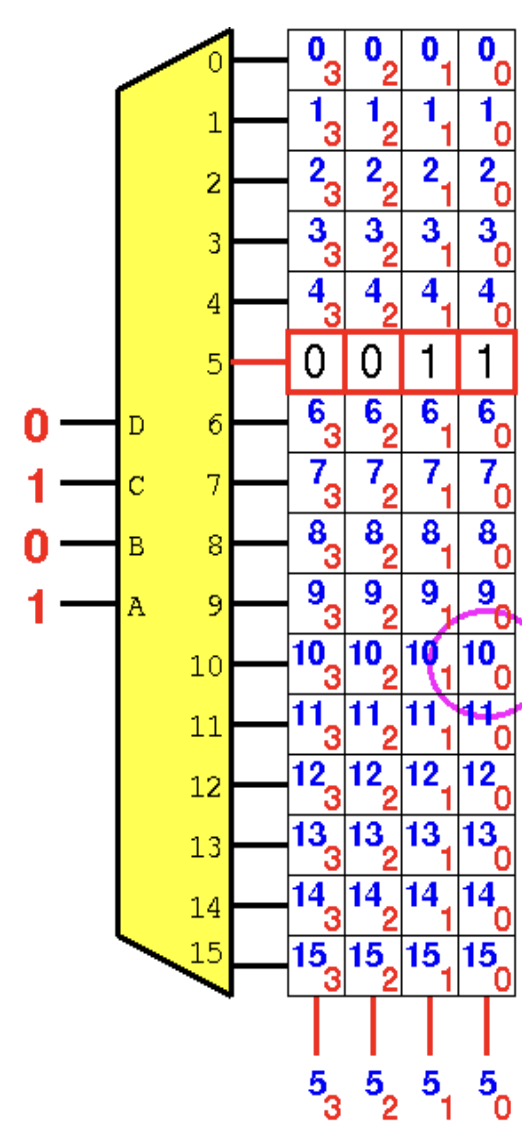
\includegraphics[width=0.45\textwidth]{chapters/chapter1c/images/structure.png}
\end{center}
\end{minipage} \\
\vfill
\begin{minipage}[htp]{0.45\textwidth}   
    \subsection{Write Operations}
    \textit{The D is connected to the Data outside of the system and at the risiing edge it updates the value of the DFF.} \textbf{The AND gate ensures that the write signal is high when the clock signal is high.} \\ \vspace*{5px}
    \begin{center}
        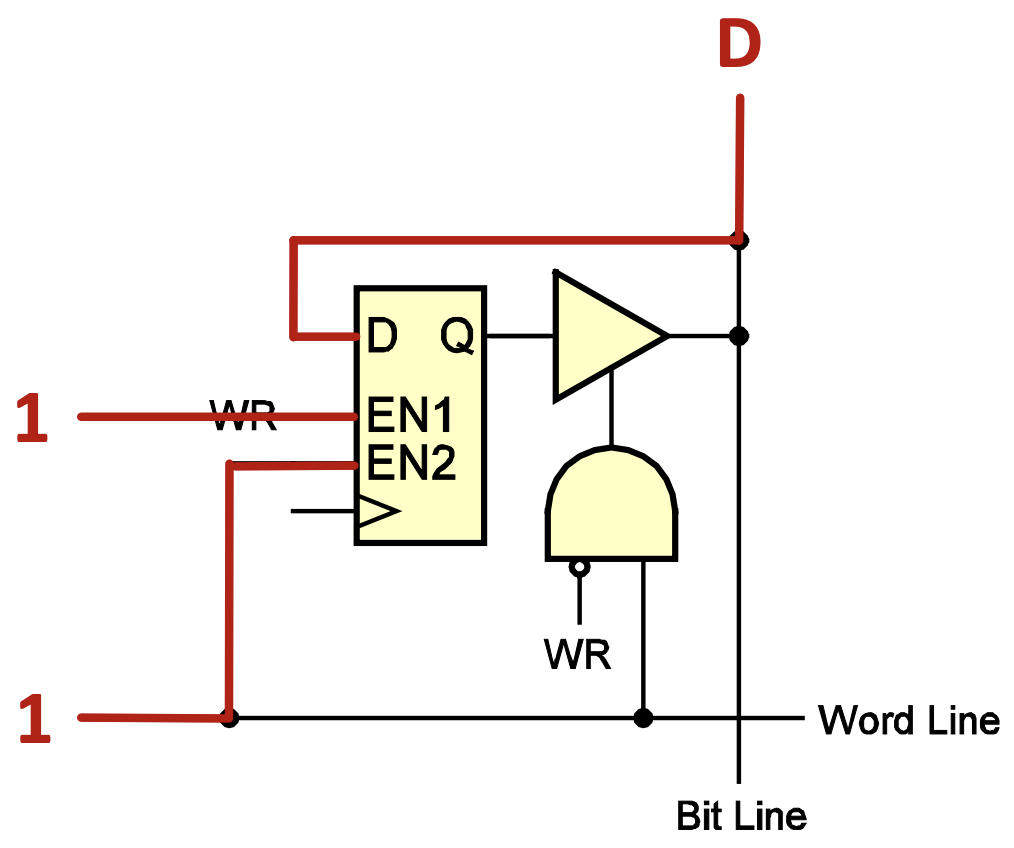
\includegraphics[width=0.45\textwidth]{chapters/chapter1c/images/write.png}
    \end{center}
\end{minipage}
\hfill  
\vline
\hfill
\begin{minipage}[htp]{0.45\textwidth}
    \subsection{Read Operations}
    \textit{D is still connected to the Data, remember the tri-state driver is active when it's enable signal is active (so when the wr is off and the operation signal is sent.).} \\ \vspace*{5px}
    \begin{center}
        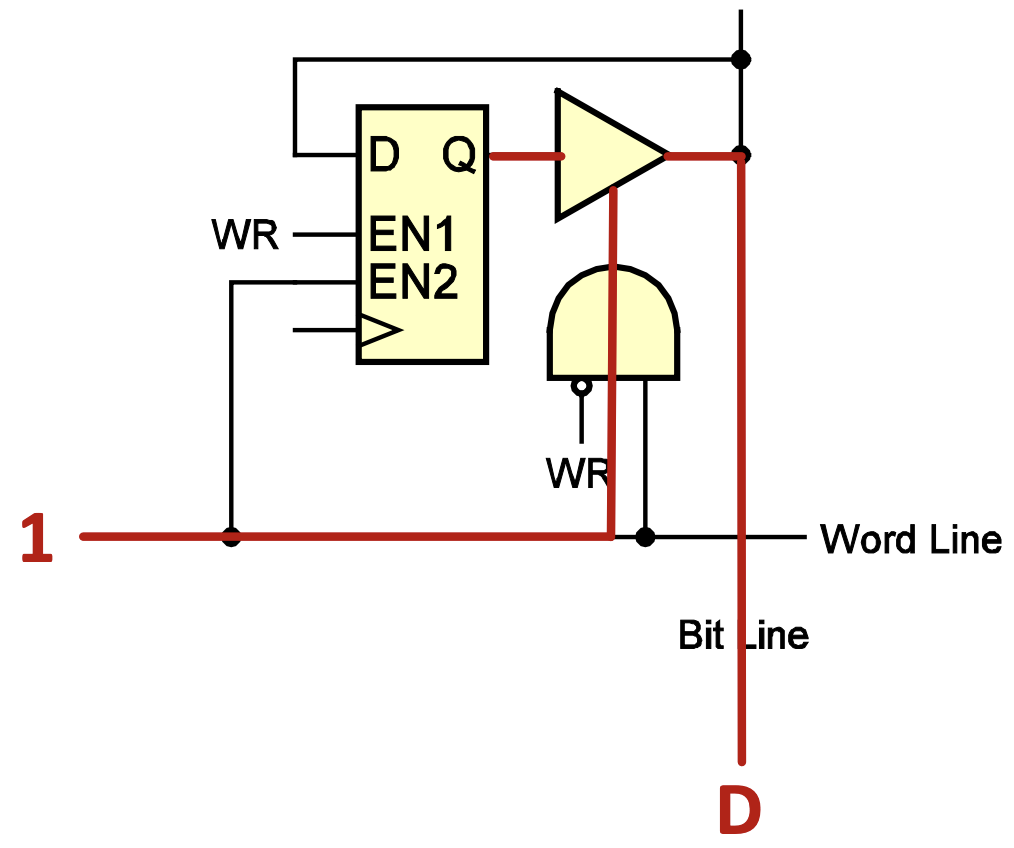
\includegraphics[width=0.45\textwidth]{chapters/chapter1c/images/read.png}
    \end{center}
\end{minipage}

\vspace*{5px}
\subsection{Practical SRAMs}
\textbf{DISCLAIMER !!: Combinational loops are prohibited as they can lead to unstable behavior, unpredictable timing, simulation and synthesis issues, excessive power consumption, and lack of a defined reset state, making them unsuitable for reliable digital circuit design.} \\ \vspace*{5px}
\textit{While the type of memory we've juste seen is small, and very fast, SRAM memories uses 6 transitors per cell (less than the previous design). We've also seen (in Taxonomy) that SRAM is \textbf{static} meaning it doesn't require periodic refresh.} \\ \vspace*{5px}
\begin{minipage}[htp]{0.45\textwidth} 
    \begin{center}
        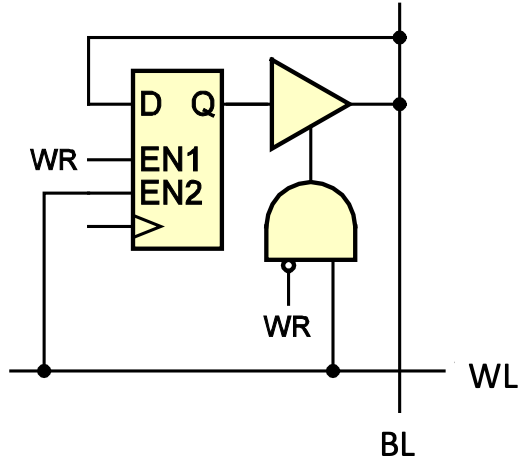
\includegraphics[width=0.55\textwidth]{chapters/chapter1c/images/ram.png}
    \end{center}
    \end{minipage}
    \hfill
    \vline
    \hfill
    \begin{minipage}[htp]{0.45\textwidth}
    \begin{center}
        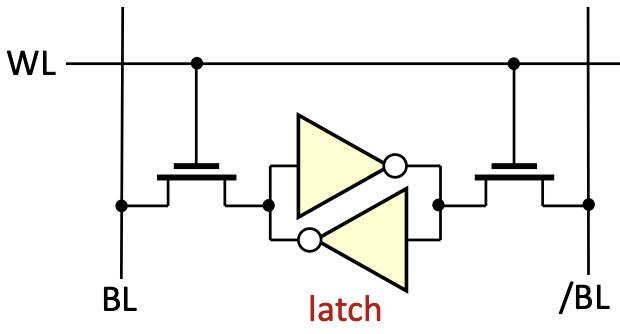
\includegraphics[width=0.55\textwidth]{chapters/chapter1c/images/sram.png}
    \end{center}
    \end{minipage}

\subsection{DRAMs}
\textit{Dynamic RAMS(DRAMs) are the densest and cheapest type of RAM memory, it stores information as charge in small capacitors. This makes the DRAM need periodic refresh otherwise the charge might leak off (~60ms) the capacitor due to parasitic resistances and the information lost} \\ \vspace*{5px}

\begin{minipage}[htp]{0.45\textwidth}
    \textbf{Refresh means, we come back before the end of a charge (~60ms) and we rewrite the value, if there is still some charge, we add charge, if there's no charge and we keep as is.} \\ \vspace*{5px}
    \textit{Personal Remark: Dynamic = Bad, data dissapears and needs refresh}
\end{minipage}
\hfill
\vline  
\hfill
\begin{minipage}[htp]{0.45\textwidth}
    \begin{center}
        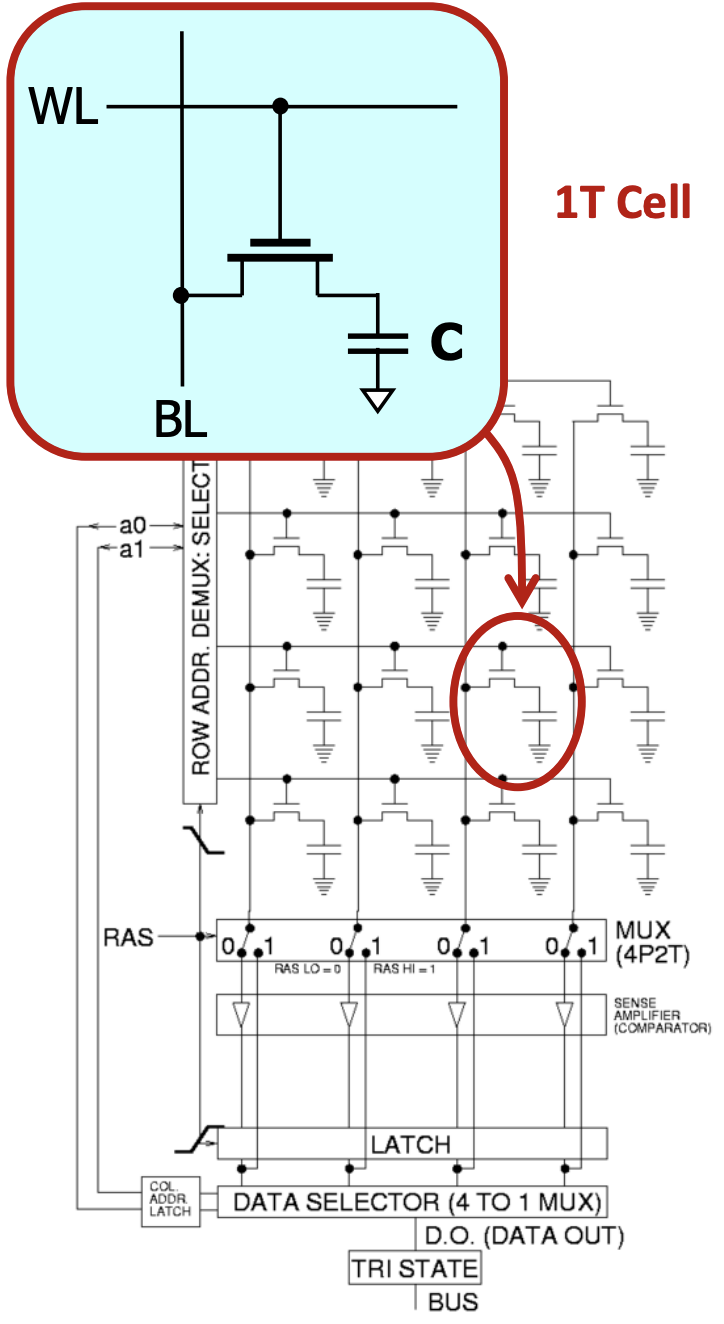
\includegraphics[width=0.5\textwidth]{chapters/chapter1c/images/dram.png}  
    \end{center}
\end{minipage}

\subsection{Ideal Random Access Memory}
\textit{A memory array uses an \(n\)-to-\(2^n\) decoder to select a word line based on the input address, enabling data to be read or written through the bit lines.}
\begin{center}
    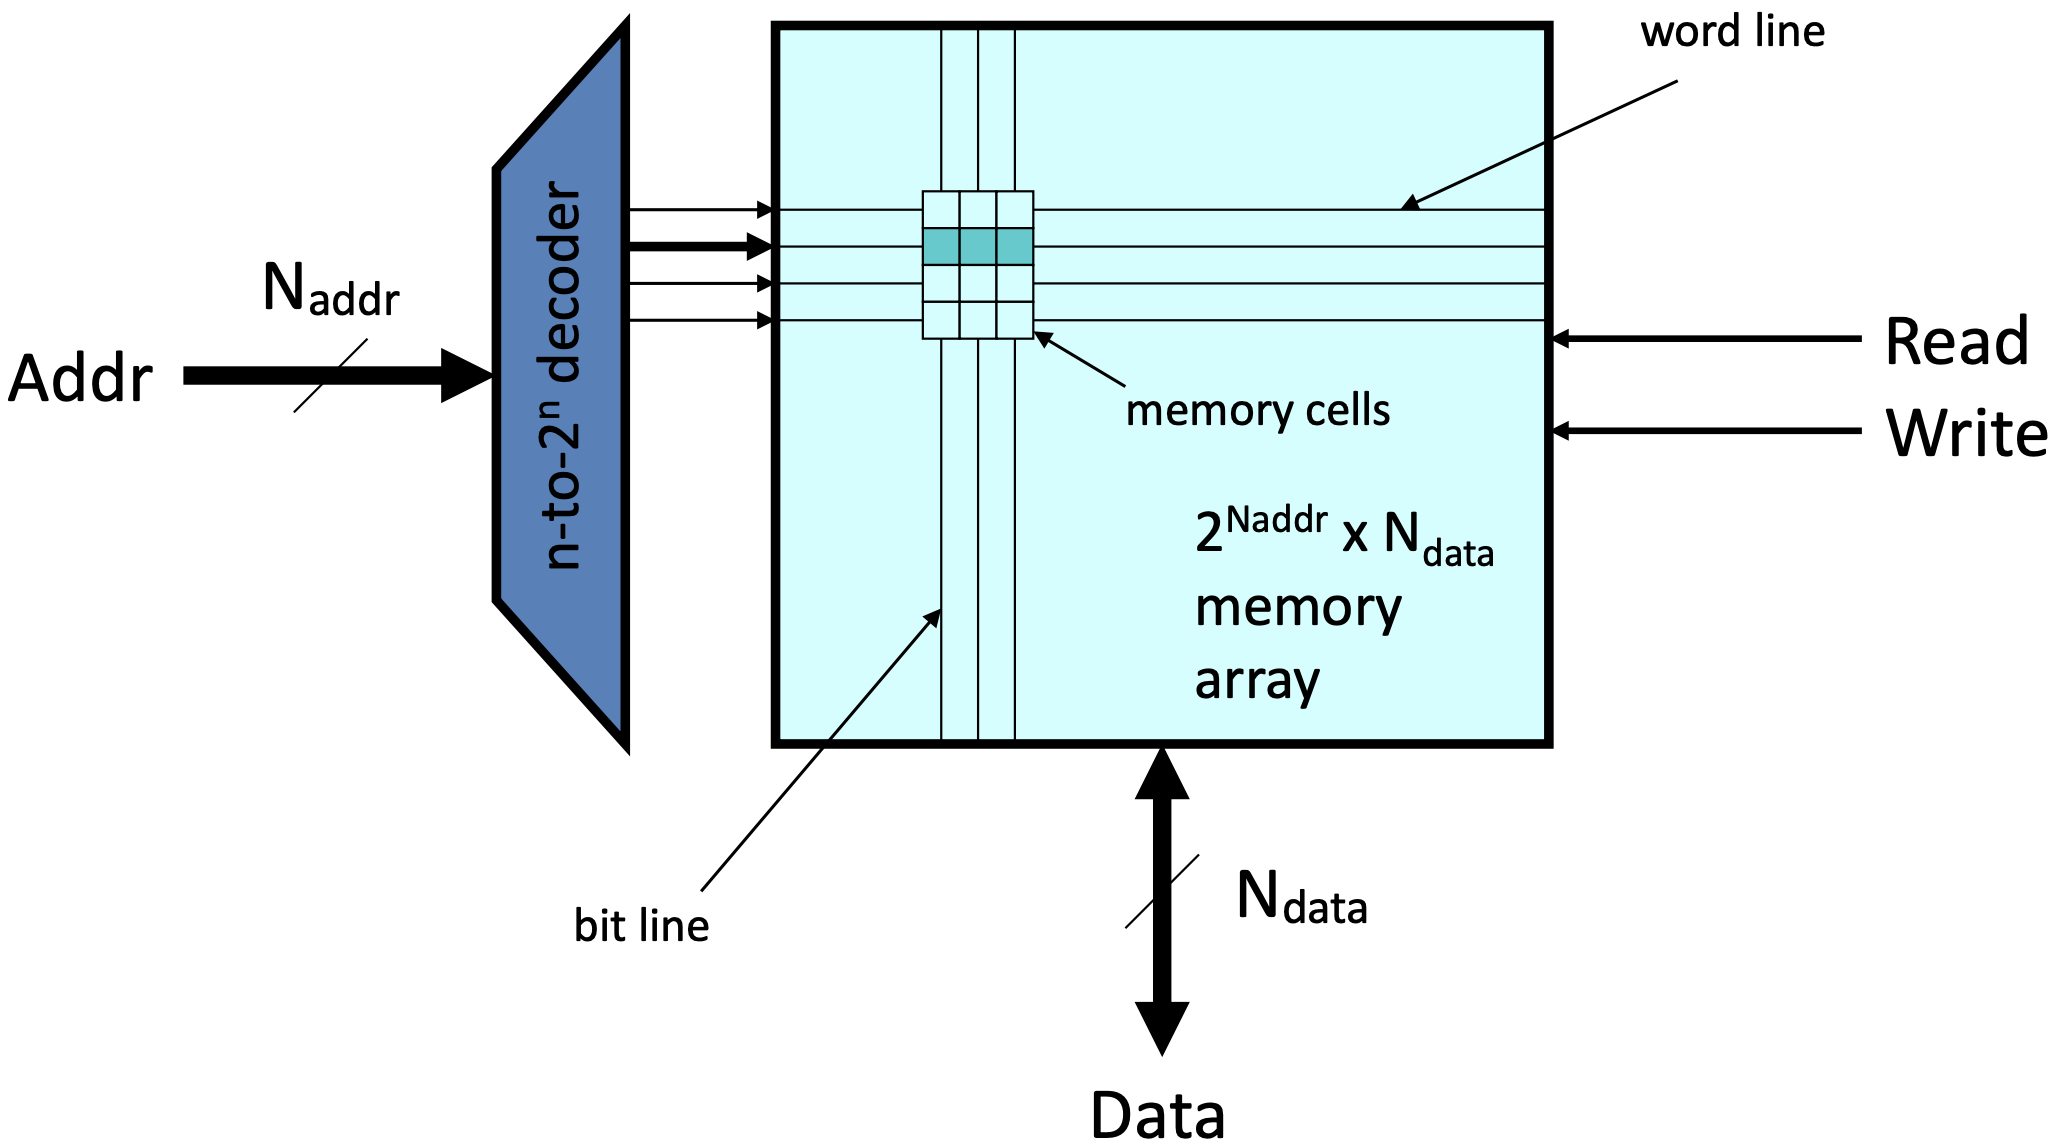
\includegraphics[width=0.45\textwidth]{chapters/chapter1c/images/ideal_ram.png}
\end{center}
\subsection{Physical Organisation }
\begin{center}
    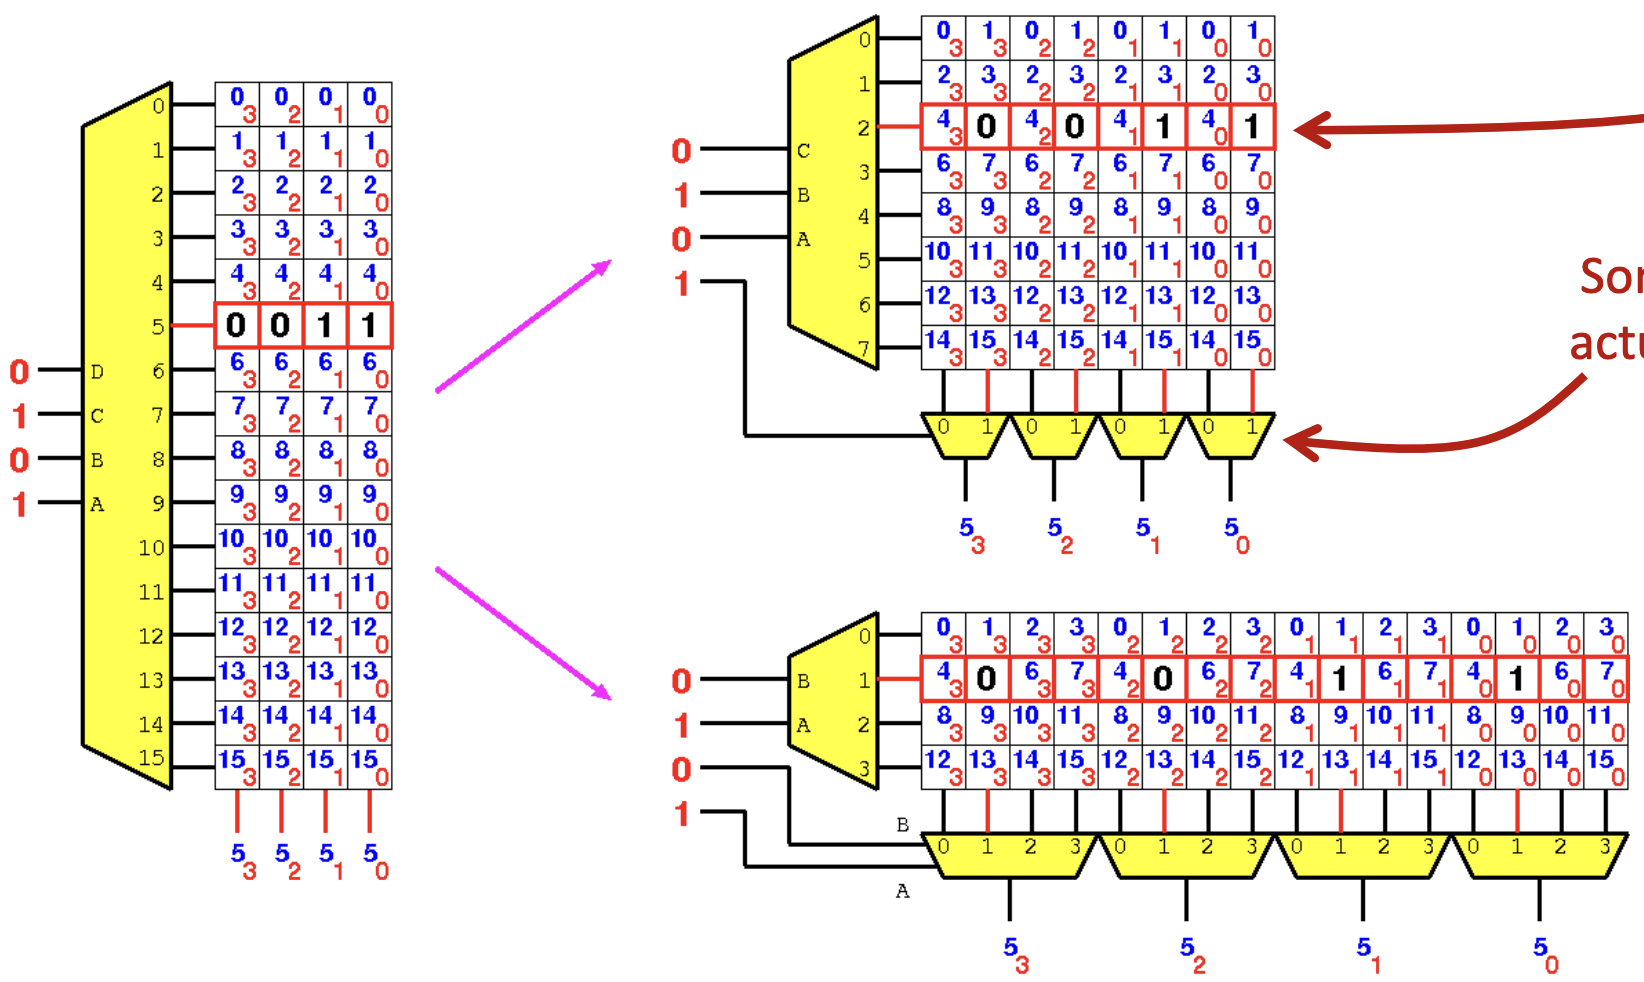
\includegraphics[width=0.45\textwidth]{chapters/chapter1c/images/organisation.png}
\end{center}
\textit{Out of all physical organizations, the squared one is the best one as it has the best performance. This layout facilitates faster access times and simplified wiring, resulting in improved computational efficiency and system scalability.}
\subsection{Realistic ROM Array}
\textit{ROMs are Read-Only Memories, they are used to store the program of the computer, they are non-volatile and can't be written to.} \\ \vspace*{5px}
\begin{center}
    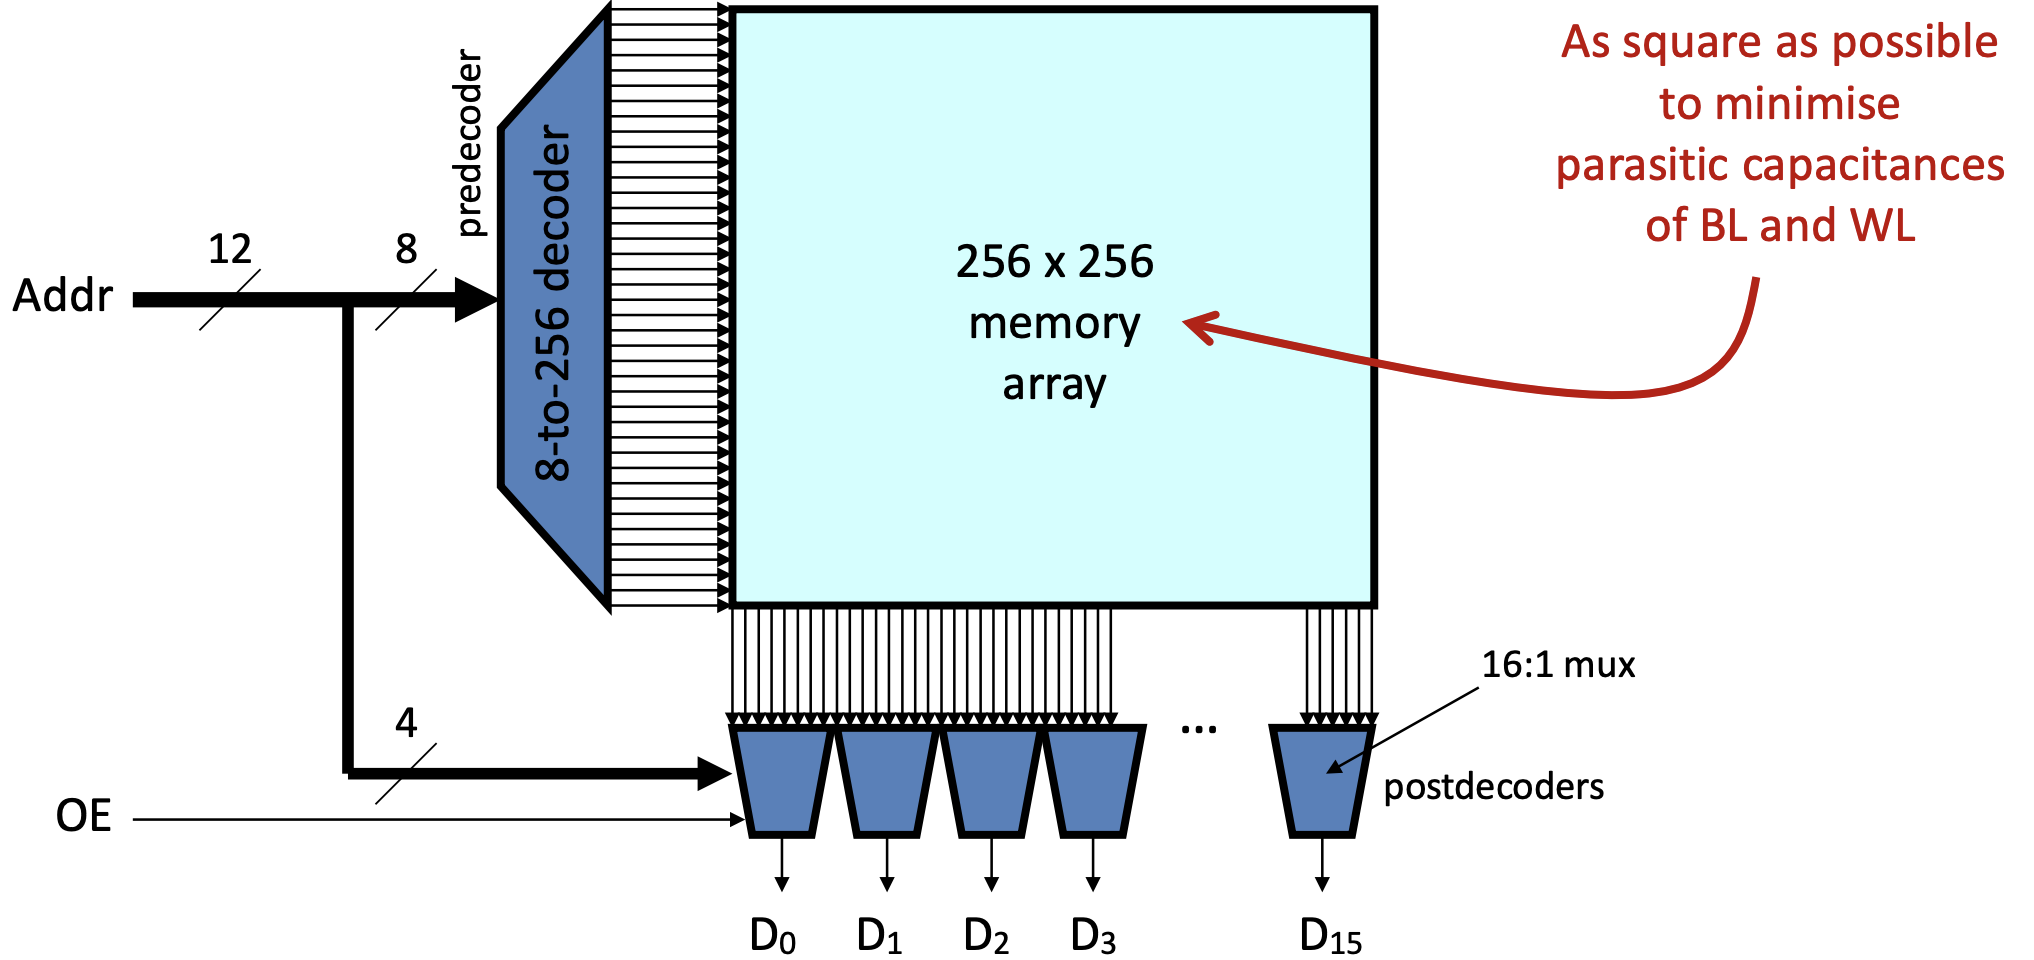
\includegraphics[width=0.45\textwidth]{chapters/chapter1c/images/rom.png}
\end{center}

\subsection{Static Ram Typical Interface}
\textit{This a typical interface of a SRAM, it has a 16-bit data input/output, a 16-bit address input, a write enable signal, and a circuit select signal.}
\begin{center}
    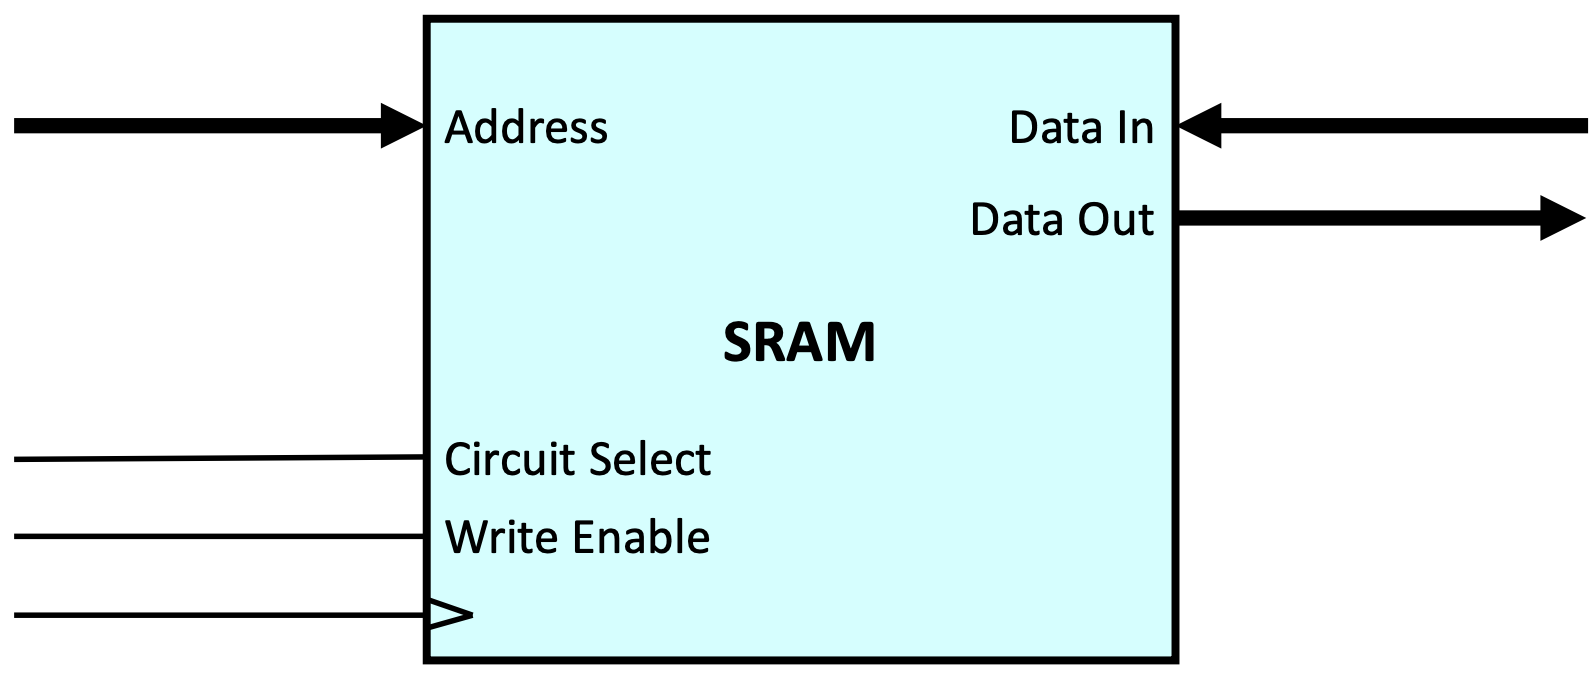
\includegraphics[width=0.45\textwidth]{chapters/chapter1c/images/sram_interface.png}
\end{center}

\section{Typical Asynchronous SRAM Read Cycle}
\textit{The read cycle of an asynchronous SRAM is initiated by the address input, which is decoded to select the word line, enabling the data to be read from the memory array and output to the data bus.} \\ \vspace*{5px}
\textit{Here, Tcyc is the cycle time, Tacc is the access time, and Ten is the enable time.}

\begin{minipage}[htp]{0.45\textwidth}
    \begin{center}
        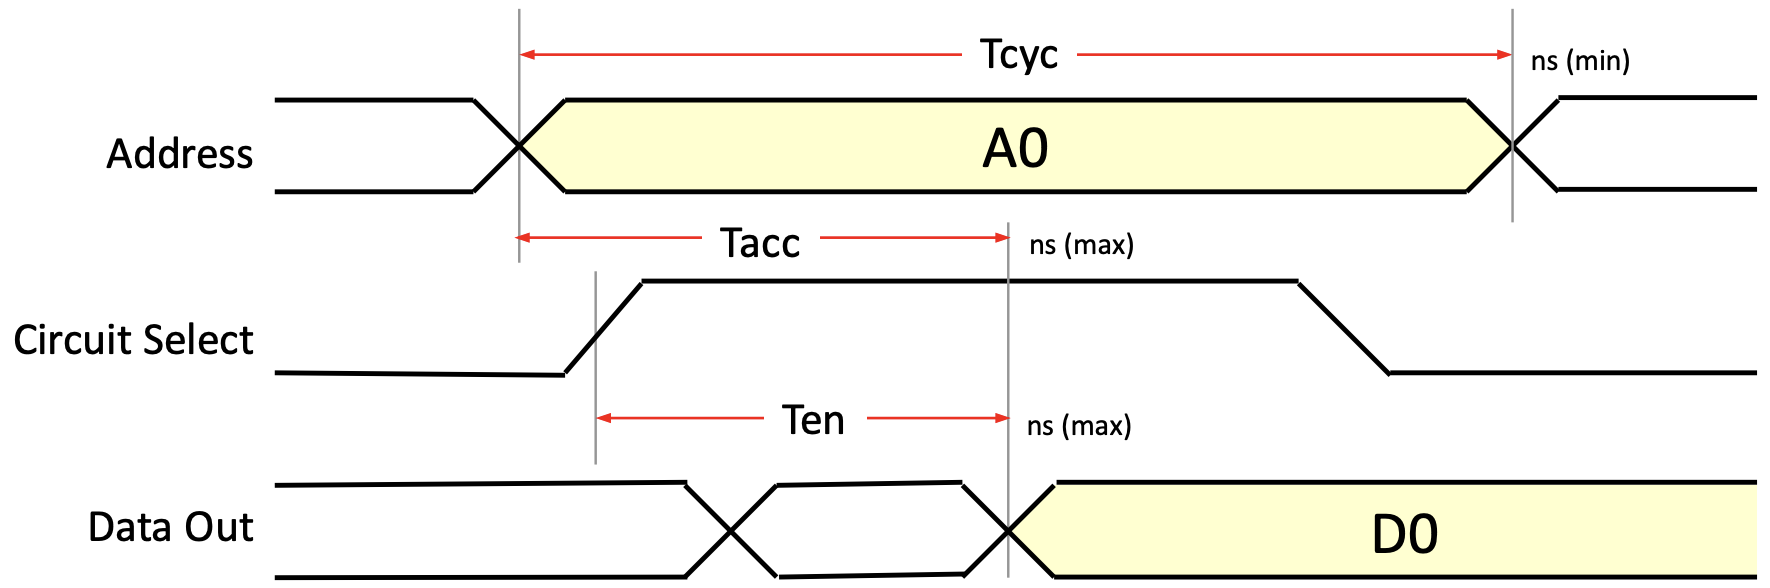
\includegraphics[width=0.45\textwidth]{chapters/chapter1c/images/sram_read.png}
    \end{center}
\end{minipage}
\hfill
\vline
\hfill
\begin{minipage}[htp]{0.45\textwidth}
    \begin{center}
        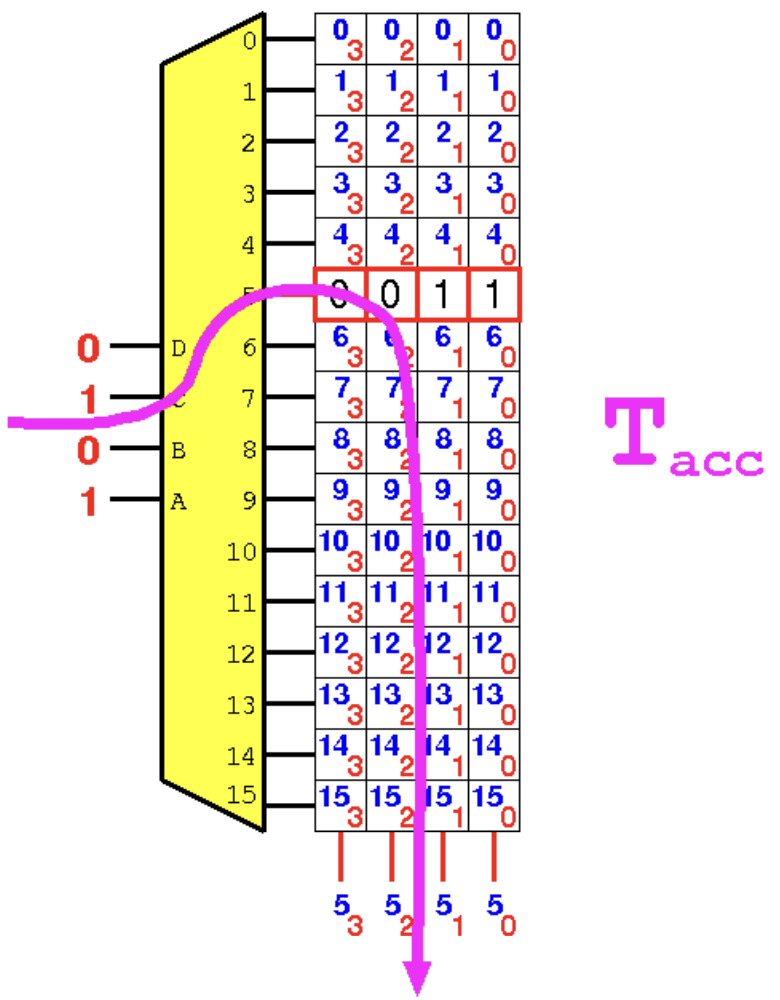
\includegraphics[width=0.45\textwidth]{chapters/chapter1c/images/sram_read2.png}
    \end{center}
\end{minipage}  

\subsubsection{Read Cycle}
\textit{Latency} defined as the number of cycles between the address asserted and data available \\ \vspace*{5px}
\begin{center}
    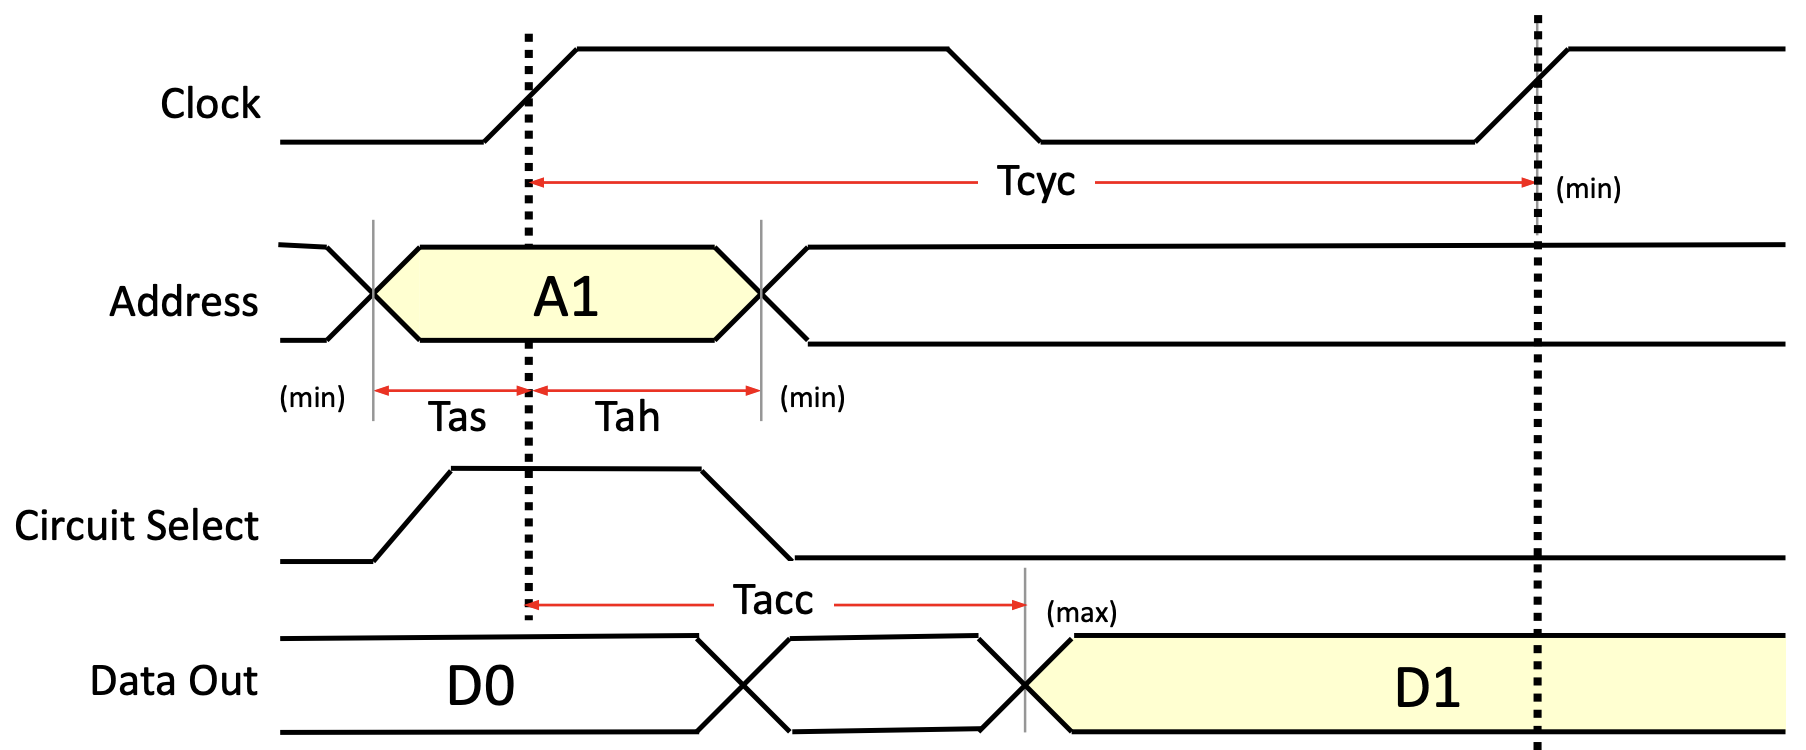
\includegraphics[width=0.45\textwidth]{chapters/chapter1c/images/read_cycle.png}
\end{center}
\subsubsection{Write Cycle}
\textit{Writes on the edge of the clock signal, as a DFF} \\ \vspace*{5px}
\begin{center}
    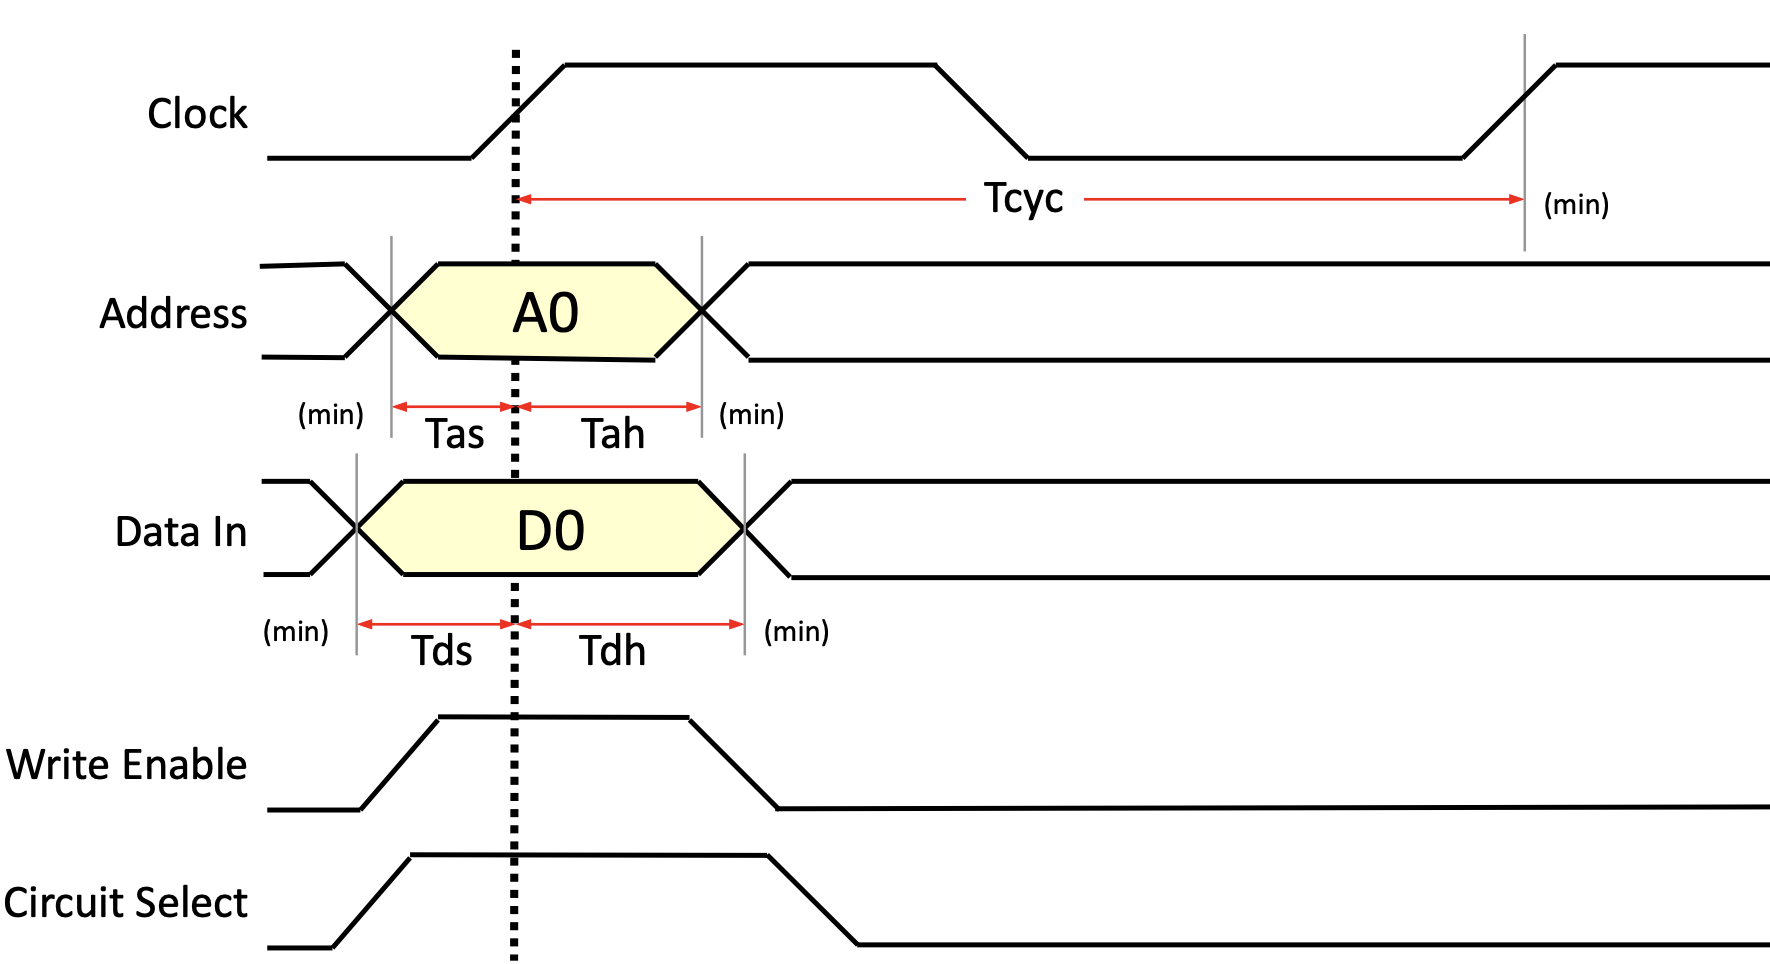
\includegraphics[width=0.45\textwidth]{chapters/chapter1c/images/write_cycle.png}
\end{center}


\section{Where is Memory in the Processor?}
\textit{In the processor we have memory in the Data memory component and in the Instruction memory component.} \\ \vspace*{5px}
\begin{center}
    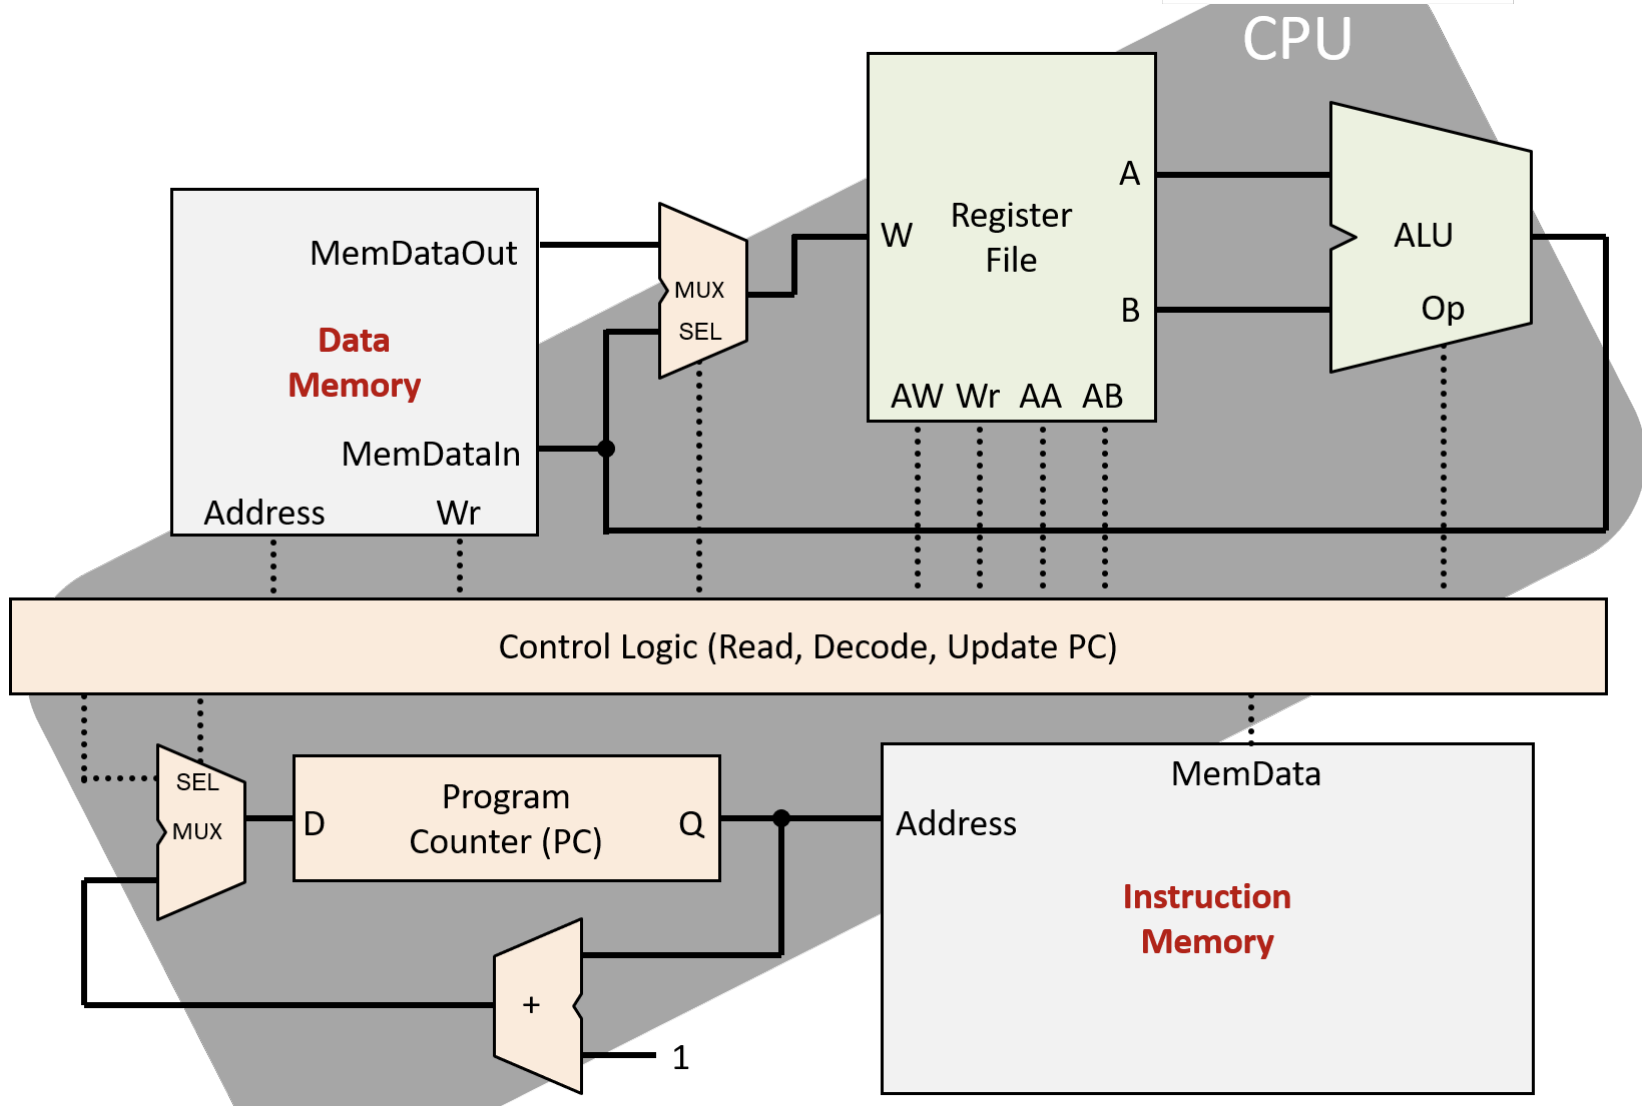
\includegraphics[width=0.45\textwidth]{chapters/chapter1c/images/processor.png}
\end{center}
\subsection{Arithmetic and Logic Instructions}
\textit{The register file can only contain a limited number of registers making it difficult to handle more complex computations and managing data input/output efficiently.}
\begin{center}
    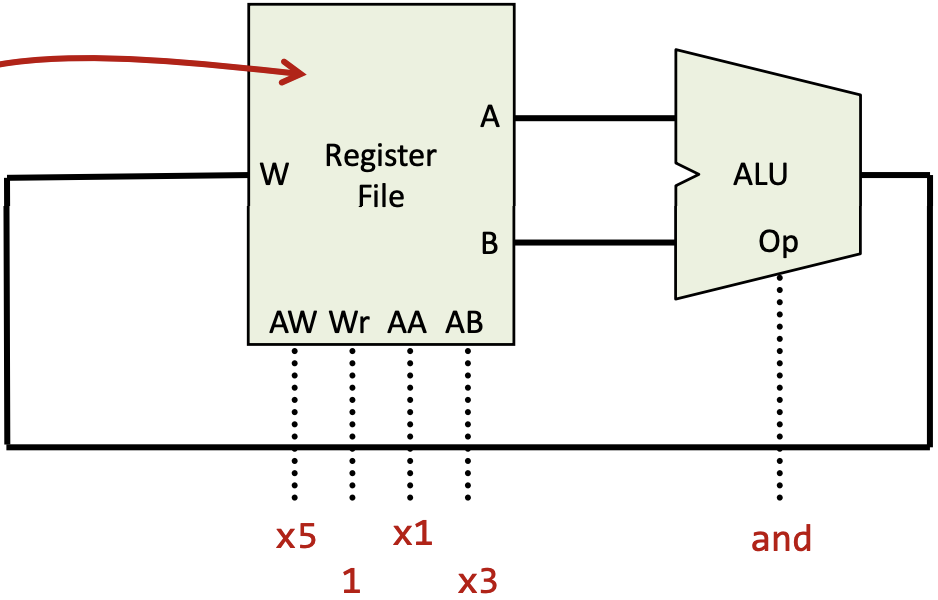
\includegraphics[width=0.45\textwidth]{chapters/chapter1c/images/arith_logic.png}
\end{center}
\subsubsection{Load Instructions}
\begin{center}
    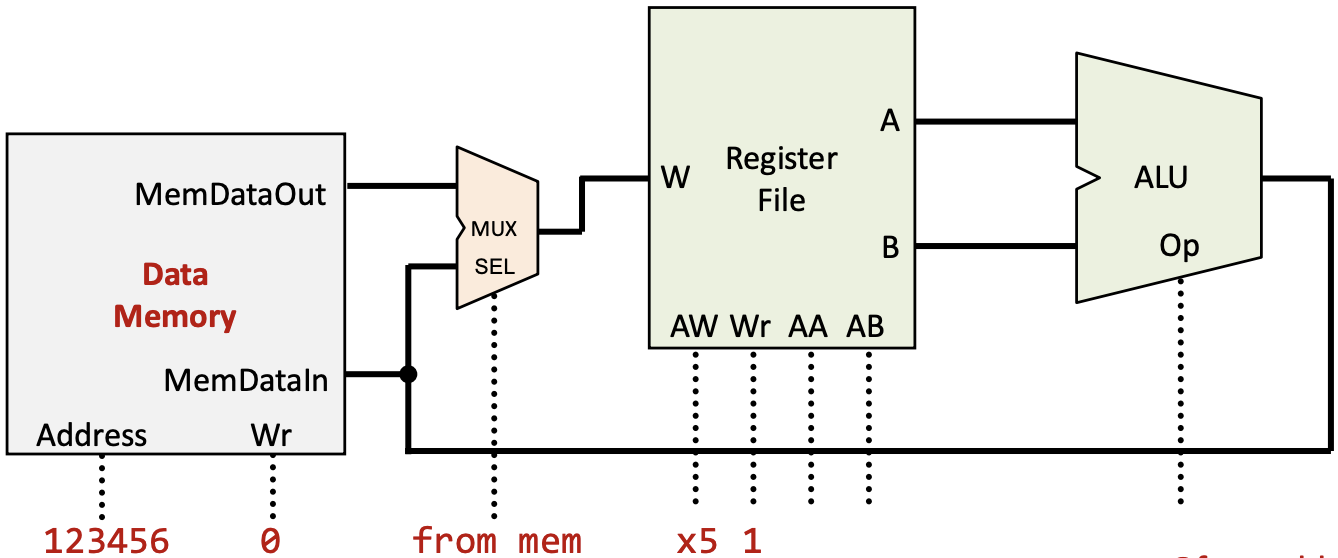
\includegraphics[width=0.45\textwidth]{chapters/chapter1c/images/load.png}
\end{center}
\subsubsection{Load and Store: The RiSC-V Way}
\textit{This instruction would never work for example because the adress is too big to be sent as an immediate value :} \texttt{lw x5, (x7)} \\ \vspace*{5px}
\begin{center}
    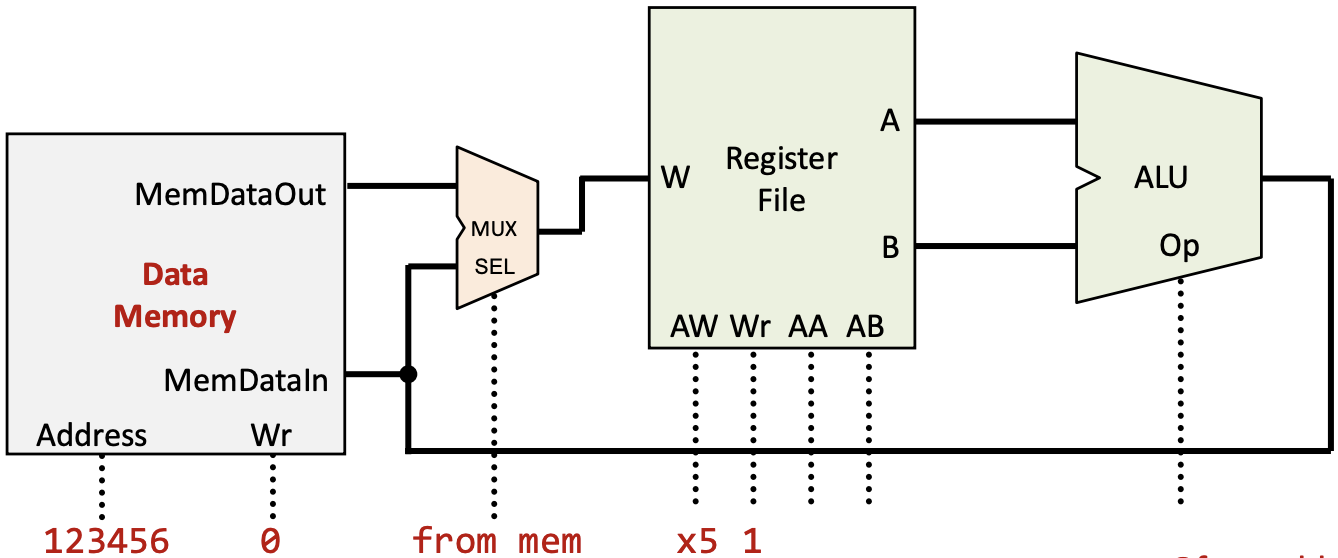
\includegraphics[width=0.45\textwidth]{chapters/chapter1c/images/load.png}
\end{center}
\subsubsection{A Load/Store Architecture}
\textit{A feature of RISC-V is that it's a Load/Store architecture, meaning that the only way to access memory is through load and store instructions. Also, instructions reading and writing in memory do exactly that and nothing else, contrary to more complex instruction set architectures (CISC), where instructions may combine memory access with other operations like arithmetic or logic. This simplicity in RISC-V's instruction set helps with streamlining the pipeline and improving performance efficiency.} \\ \vspace*{5px}

\begin{center}
    \begin{tabular}{|c|c|c|c|c|}
        \hline
        \multicolumn{2}{|c|}{\textbf{Load}} & \textbf{I} & 0x2 & 0x03 \\ 
        \hline
        \texttt{lw} & \texttt{rd,imm(rs1)} & \multicolumn{3}{c|}{\texttt{rd $\leftarrow$ mem[rs1 + sext(imm)]}} \\ 
        \hline
        \multicolumn{2}{|c|}{\textbf{Store}} & \textbf{S} & 0x2 & 0x23 \\ 
        \hline
        \texttt{sw} & \texttt{rs2,imm(rs1)} & \multicolumn{3}{c|}{\texttt{mem[rs1 + sext(imm)] $\leftarrow$ rs2}} \\ 
        \hline
    \end{tabular}
\end{center}

\section{More Addressing Modes? Not in RISC-V!}
\vspace*{-10px}
\begin{center}
\resizebox{1.1\textwidth}{!}{
\begin{tabular}{|l|l|l|}
\hline
\textbf{Addressing Mode}          & \textbf{Instruction}                                      & \textbf{Description}                                                                                   \\ \hline
\textbf{Register}                 & \texttt{add x0, x1, x2}                                   & Adds the value of \texttt{x1} and \texttt{x2}, stores the result in \texttt{x0}.                         \\ \hline
\textbf{Immediate}                & \texttt{add x0, x1, 123}                                  & Adds the value of \texttt{x1} and the immediate constant 123, stores the result in \texttt{x0}.          \\ \hline
\textbf{Direct or Absolute}       & \texttt{add x0, x1, (1234)}                               & Adds the value of \texttt{x1} and the value at memory address 1234, stores the result in \texttt{x0}.    \\ \hline
\textbf{Register Indirect}        & \texttt{add x0, x1, (x2)}                                 & Adds the value of \texttt{x1} and the value in memory at the address held in \texttt{x2}, stores in \texttt{x0}. \\ \hline
\textbf{Displacement or Relative} & \texttt{add x0, x1, 123(x2)}                              & Adds the value of \texttt{x1} and the value in memory at \texttt{x2} plus the displacement 123, stores in \texttt{x0}. \\ \hline
\textbf{Base or Indexed}          & \texttt{add x0, x1, i5(x2)}                               & Adds the value of \texttt{x1} and the value in memory at \texttt{x2} plus index \texttt{i5}, stores in \texttt{x0}. \\ \hline
\textbf{Auto-increment/-decrement} & \texttt{add x0, x1, (x2+)}                               & Adds the value of \texttt{x1} and the value in memory at the address in \texttt{x2}, then increments \texttt{x2}, stores in \texttt{x0}. \\ \hline
\textbf{PC-Relative}              & \texttt{add x0, x1, 123(pc)}                              & Adds the value of \texttt{x1} and the value in memory at \texttt{pc} plus 123, stores in \texttt{x0}.    \\ \hline
\end{tabular}}
\end{center}
    
\textit{Syntax here looks like RISC-V but most of these instructions do not exist in RISC-V.}
\newpage
\subsection{Word Adressed Memory}
\textit{In a word addressed memory, the address is the index of the word in the memory.} \\ 
\textit{The letters inside the word are identified as eg. for Hello World, H:3980, E:3981, L:3982, \dots}.
\begin{center}
    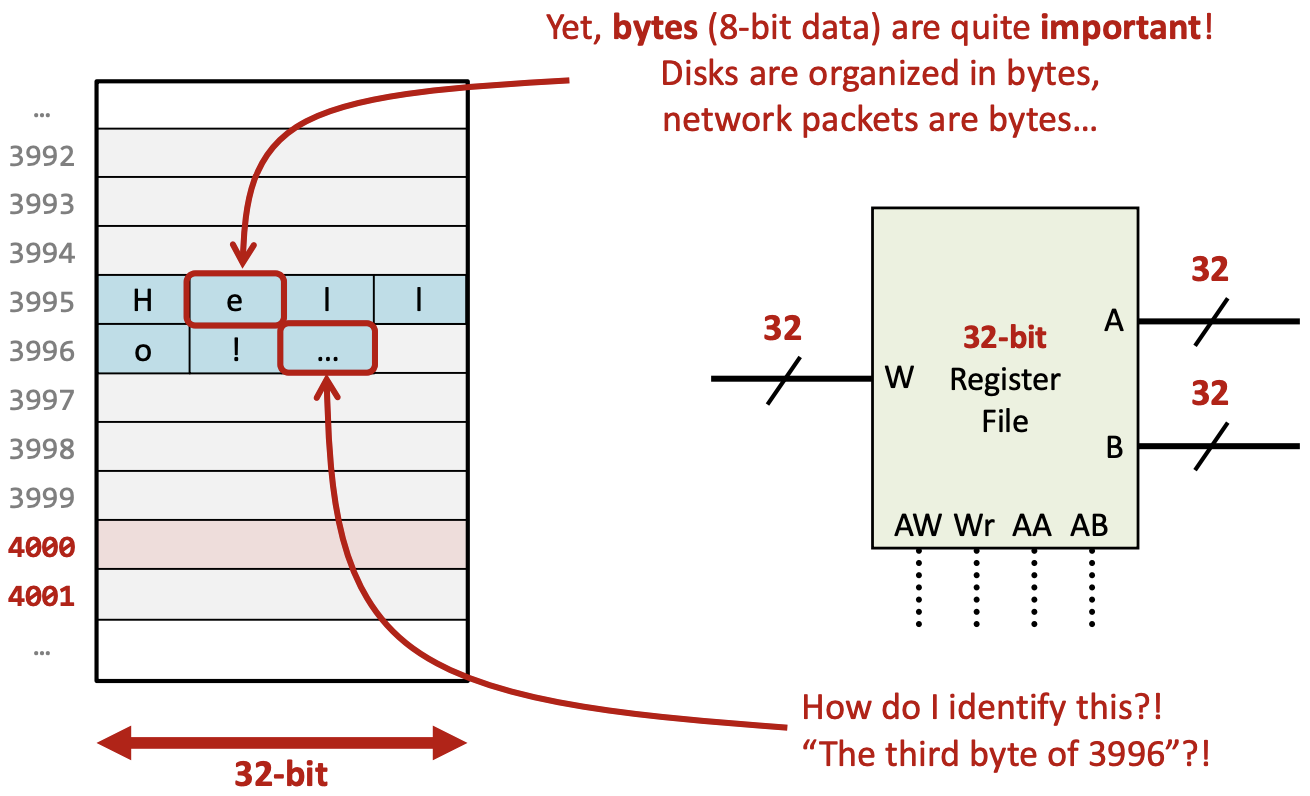
\includegraphics[width=0.45\textwidth]{chapters/chapter1c/images/word_add.png}
\end{center}

\subsection{Loading Words (lw) and Instructions}
\textit{The lw instruction is used to load a word from memory into a register.} \\ 
\textit{The adress of such words would necessarly be a multiple of 4 meaning the two least significant bits must be 0s.(to the ensure the data is word aligned\dots)} \\ 
\begin{center}
    \includegraphics[width=0.45\textwidth]{chapters/chapter1c/images/lw.png}
\end{center}
\subsection{Loading Bytes (lb)}
\textit{The \texttt{lb} (Load Byte) instruction doesn't require alignment because it only loads 1 byte (8 bits), which can be accessed at any memory address, unlike \texttt{lw} which requires word alignment to efficiently load 4 bytes (32 bits).
}\textit{The lb instruction is used to load a byte from memory into a register.} \\ 

\begin{center}
    \includegraphics[width=0.45\textwidth]{chapters/chapter1c/images/lb.png}
\end{center}
\subsection{A Few More Load/Store Instructions}
\textit{Access bytes (and half-words) as if memory were made of bytes}
\begin{center}
    \includegraphics[width=0.45\textwidth]{chapters/chapter1c/images/lb.png}
\end{center}
\subsection{Access as it is more suitable}
\textit{For example storing the "Hello!"zero value in the memory would like this:} \\
\begin{minipage}[htp]{0.45\textwidth}
    \begin{center}
        \includegraphics[width=0.45\textwidth]{chapters/chapter1c/images/hello.png}
    \end{center}
\end{minipage}
\hfill
\vline
\hfill
\begin{minipage}[htp]{ .45\textwidth}
    \begin{center}
        \includegraphics[width=0.3\textwidth]{chapters/chapter1c/images/hello2.png}
    \end{center}
\end{minipage}
\subsubsection{Counting Characters in a String}
\textit{As an example, for counting the number of characters in a string, the load byte instruction would be more suitable as seeing the string as a sequence of bytes makes use of the memory as a sort of array.} \\ \vspace*{5px}

\begin{center}
    \includegraphics[width=0.15\textwidth]{chapters/chapter1c/images/hello2.png}
\end{center}
\begin{center}
    \begin{assembly}
strlen:
    mv t0, a0 # Copy the pointer (a0) into t0 to traverse the string
    li t1, 0 # t1 will hold the length (initialized to 0)
loop:
    lbu t2, 0(t0) # Load byte at address t0 into t2
    beq t2, zero, end # If t2 is 0 (null byte), we are done
    addi t1, t1, 1 # Increment the length counter (t1)
    addi t0, t0, 1 # Point to the next character in the string
j loop # Repeat the loop
end:
    mv a0, t1 # Move the length (t1) into a0 as the return value
    ret # Return to caller
    \end{assembly}
\end{center}

\textit{\texttt{lbu} is used here to ensure that the byte is treated as an unsigned value, which is the correct approach for processing characters in a string.
}
\newpage
In a word addressed memory view, the code would look like such: \\ \vspace*{5px}
\begin{center}
\begin{assembly}
strlen:
    li t1, 0           # t1 will hold the length (initialized to 0)
next_word:
    li t2, 4           # t2 will count the bytes in a loaded word (four)
    lw t3, 0(t0)       # Load four bytes at address t0 into t3
next_byte:
    andi t4, t3, 0xff  # Move the "little-end" in t4
    beq t4, zero, end  # If t4 is 0 (null byte), we are done
    addi t1, t1, 1     # Increment the length counter (t1)
    srli t3, t3, 8     # Prepare the next byte of the word in the "little-end" (t3)
    addi t2, t2, -1    # One byte left in the loaded word
    bnez t2, next_byte # If more bytes in t3, check the next
    addi a0, a0, 4     # Else point to the next word of characters in the string
    j next_word        # Repeat the loop
end:
    mv a0, t1          # Move the length (t1) into a0 as the return value
    ret                # Return to caller
\end{assembly}
\end{center}
\subsection{Loading Bytes (lb)}
\textit{Now, one may wonder in what ordering the bytes are stored in memory.} \\ \vspace*{5px}
\begin{center}
    \includegraphics[width=0.55\textwidth]{chapters/chapter1c/images/lb.png}
\end{center}
\subsubsection{Which Byte Where?}
\textit{Both ordering of bytes are valid the only thing we have to do is stick to one, the most generally used is little-endian as it's the RISCV default and the Intel x86/x64 default.} \\ \vspace*{5px}
\begin{minipage}[htp]{0.45\textwidth}
    \begin{center}
        \textbf{Little Endian} \\ \vspace*{5px}
        \includegraphics[width=0.55\textwidth]{chapters/chapter1c/images/bytes.png}
    \end{center}   
\end{minipage}
\hfill
\vline
\hfill
\begin{minipage}[htp]{0.45\textwidth}
    \begin{center}
        \textbf{Big Endian} \\ \vspace*{5px}
        \includegraphics[width=0.55\textwidth]{chapters/chapter1c/images/bytes2.png}
\end{center}
\end{minipage} \\ \vspace*{5px}
\begin{center}
    \includegraphics[width=0.85\textwidth]{chapters/chapter1c/images/final_endian.png} \\
    \href{https://www.google.com/url?sa=i&url=https%3A%2F%2Fmedium.com%2Fmycsdegree%2Fsockets-in-c-little-and-big-endian-machines-23c9ed484c20&psig=AOvVaw1P8zdPW_G0ioJC2Ka6cOX5&ust=1731236021875000&source=images&cd=vfe&opi=89978449&ved=0CBQQjRxqFwoTCPinlvaKz4kDFQAAAAAdAAAAABAJ}{source}
\end{center}
\textit{Personal Remark : Mnemotechnic - Little Endian = Little End (The ending memory index takes the smallest(starting) data adress), Big Endian = Big End.}
\textit{Or, Little Endian = LSB in smallest index, Big Endian = MSB in smallest index.} % Including chapter0.tex from chapters folder
\chapter{Part I(d) - ISA Arrays and Data Structures - W 2.2}
\section{Arrays}
\textit{In higher level languages, are written like follows :}
\begin{java}
short\[\] myData = \{10407, -16533, -22715, 29796, 18956, \dots\}:
\end{java}
\subsection{Different Ways to Store Arrays}
\begin{center}
    \includegraphics[width=0.45\textwidth]{chapters/chapter1d/images/arrays.png}
\end{center}
\begin{itemize}
\item \textbf{A: Storing Arrays with a Null Terminator}
\begin{itemize}
    \item[-] In this method, the array is stored with each element represented using 16-bit integers.
    \item[-] A null terminator (the value 0) is used at the end of the array to indicate its termination.
    \item[-] This method is common when the array size is unknown in advance, and the null terminator acts as a signal to stop reading the data.
\end{itemize}

\item \textbf{B: Storing Arrays with a Length Prefix}
\begin{itemize}
    \item[-] Here, the first element of the array contains the length of the array, stored as a 16-bit integer (in this case, the length is 9).
    \item[-] The rest of the array is stored in consecutive memory locations, similar to method A.
    \item[-] This method allows the array size to be known before reading all the data, making it more efficient for some use cases.
\end{itemize}

\item \textbf{C: Storing Arrays without a Terminator or Length Prefix}
\begin{itemize}
    \item[-] In this case, the array is stored without a length prefix or a null terminator.
    \item[-] The size of the array must be known externally, either through the code or an external mechanism.
    \item[-] This method is the most compact but requires prior knowledge of the array's size.
\end{itemize}
\end{itemize}

\subsection{Adding Positive Elements}
\textit{Here we'll write the same program for the different ways of storing arrays.} \\
\textit{The program will add all positive elements of an array of signed 16-bit integers. At call time, a0 points to the array, at return time, a0 contains the result.} \\

\textbf{A: Storing Arrays with a Null Terminator}\\
\begin{center}
    \includegraphics[width=0.14\textwidth]{chapters/chapter1d/images/A.png}
\end{center}

\begin{center}
\begin{assembly}
add_pos:li t0, 0         # Initialize t0 to 0
        lh t1, 0(a0)     # Load halfword from memory address a0 into t1
        beqz t1, end     # Branch to 'end' if t1 equals zero
        blez t1, donothing  # Branch to 'donothing' if t1 is less than or equal to zero
        add t0, t0, t1   # Add t1 to t0 (only if t1 is positive)
donothing:               # This block does nothing for negative or zero values
# You can put other operations here if needed
        j add_pos        # Jump back to the beginning of add_pos to check the next value
end:                     # Label 'end' for the program termination
\end{assembly}
\end{center}
\textbf{B: Storing Arrays with a Length Prefix} \\
\begin{center}
    \includegraphics[width=0.14\textwidth]{chapters/chapter1d/images/B.png}
\end{center}

\begin{center}
\begin{assembly}
add_pos_b:  
    lh t2, 0(a0)        # Load the length of the array into t2
    addi a0, a0, 2      # Move to the first element of the array (skip the length prefix)
    li t0, 0            # Initialize t0 to 0 for storing the sum
loop_b:    
    beqz t2, end_b      # If the length (t2) is zero, branch to 'end_b'
    lh t1, 0(a0)        # Load the current array element into t1
    blez t1, skip_b     # If t1 is less than or equal to zero, skip the addition
    add t0, t0, t1      # Add t1 to t0 (only if t1 is positive)
skip_b:    
    addi a0, a0, 2      # Move to the next element in the array
    addi t2, t2, -1     # Decrease the length counter
    j loop_b            # Jump back to loop_b
end_b:                  # End label
\end{assembly}
\end{center}
\textbf{C: Storing Arrays without a Terminator or Length Prefix} \\
\begin{center}
    \includegraphics[width=0.14\textwidth]{chapters/chapter1d/images/C.png}
\end{center}

\begin{center}
\begin{assembly}
add_pos_c:  
    li t0, 0         # Initialize t0 to 0 for storing the sum
loop_c:     
    beqz t2, end_c   # If the array size (t2) is zero, branch to 'end_c'
    lh t1, 0(a0)     # Load the current array element into t1
    blez t1, skip_c  # If t1 is less than or equal to zero, skip the addition
    add t0, t0, t1   # Add t1 to t0 (only if t1 is positive)
skip_c:    
    addi a0, a0, 2   # Move to the next element in the array
    addi t2, t2, -1  # Decrease the array size counter
    j loop_c         # Jump back to loop_c
end_c:               # End label
\end{assembly}
\end{center}

\subsection{Pointer to Memory vs Index in Array}
\textit{Now we're wodnering which one of these two ways of accessing the array is better.} \\
\textbf{Obviously the less instructions the better (not always true actually but well),\\ Pointer to Memory.} \\
\begin{minipage}[htpb]{0.45\textwidth}
\begin{assembly}
add_positive:
    li t0, 0
    mv t1, a1
next_short:
    beq t1, zero, end
    lh t2, 0(a0)
    bltz t2, negative
    add t0, t0, t2
negative:
    addi a0, a0, 2
    addi t1, t1, -1
    j next_short
end:
    mv a0, t0
ret
\end{assembly}
\end{minipage}
\hfill
\vline
\hfill
\begin{minipage}[htp]{0.45\textwidth}
\begin{assembly}
add_positive:
    li t0, 0
    li t1, 0
next_index:
    bge t1, a1, end
    slli t2, t1, 1
    add t2, a0, t2
    lh t3, 0(t2)
    bltz t3, negative
    add t0, t0, t3
negative:
    addi t1, t1, 1
    j next_index
end:
    mv a0, t0
ret
\end{assembly}
\end{minipage}
\newpage
\subsubsection{In C}
\textit{Writing this in C for better understanding. Again, which one is better?} \\
\vspace*{5px}
\textbf{Obviously the less instructions the better (again not always true but ah), Index in array} \\
\begin{minipage}[htp]{0.45\textwidth}
\textbf{Pointer to memory} \\
\begin{cc}
short sum = 0;
short *ptr = myData;
short *end = myData + N;
while (ptr < end) {
    if (*ptr > 0) {
    sum += *ptr;
}
    ptr++;
}
\end{cc}
\end{minipage}
\hfill
\vline
\hfill
\begin{minipage}[htp]{0.45\textwidth}
\textbf{Index in array} \\
\begin{cc}
short sum = 0;
int i;
for (i = 0; i < N; i++) {
    if (myData[i] > 0) {
    sum += myData[i];
}
}
\end{cc}
\end{minipage}

\subsubsection{We need a good compiler}
\textit{Seeing this, the idea would be to have a sufficiently good \textbf{compiler} (check I.4.3.2 if needed) such that we write our C code in Index in array, and we get Pointer to memory code in assembly. Thus writing better code but also getting better performance.} \\
\textbf{Another type of collection we could've used to store the data is a \textit{Linked List}.} \\
\vspace*{5px}
\begin{minipage}[htp]{0.45\textwidth}   
    \textit{Linked lists are useful for efficiently inserting and deleting elements, especially in the middle of the list.} \\
    \vspace*{5px}
    \textit{Each 32-bit element in a linked list contains 16 bits for the value and 16 bits for the address of the next element, enabling efficient insertions but slower sequential access compared to arrays.}
\end{minipage}
\hfill
\vline
\hfill
\begin{minipage}[htp]{0.45\textwidth}
\begin{center}
    \includegraphics[width=0.95\textwidth]{chapters/chapter1d/images/linked_list.png}
\end{center}
\end{minipage} % Including chapter0.tex from chapters folder

\chapter{Part I(e) - ISA Arithmetic - W 3.1}
\section{Notation}
Before we start, let's define some notation:
\begin{itemize}
    \item[-] \textbf{Number representation (with a fixed number of digits/bits):}
    \[
    A = A^{(n)} = A^{(m)}
    \]
    
    \item[-] \textbf{Number in binary or decimal:}
    \[
    A = A_{10} = A_{2} = A_{2c}
    \]
    \textit{With $A_{2c}$ being the 2's complement representation.} \\
    \textit{And $A_{2}$ being the binary representation.}
    \item[-] \textbf{Individual digits or bits:}
    \[
    a_{n-1}, a_{n-2}, \dots, a_2, a_1, a_0
    \]
    
    \item[-] \textbf{Digit string representation:}
    \[
    \langle a_{n-1} a_{n-2} \dots a_2 a_1 a_0 \rangle
    \]
\end{itemize}

\section{Numbers}

Numbers in computing can be represented in different forms, each with specific use cases. \\
\vspace*{5px}
\textbf{Integers} can be either signed or unsigned, representing positive and negative values, or only non-negative values. Examples include:
\[
0, 1, 2, 3, 4294967295, -2147483648
\]

\textbf{Fixed-point} numbers are essentially integers with an implicit scaling factor (e.g., \(10^k\) or \(2^k\)) to handle fractional values. Common in applications like signal processing. Examples include:
\[
0.12, 3.14, 1073741823.75
\]

\textbf{Floating-point} numbers represent a wide range of values using a base and exponent, providing flexibility in precision. Examples include:
\[
3.14E3, -2.5E1, 1.0E0, 4.2E-2, -1.5E-3
\]

\subsection{Unsigned Integers}
Unsigned integers are:
\begin{itemize}
    \item[-] \textit{Weighted}: Each digit has a positional value.
    \item[-] \textit{Nonredundant}: Every number has a unique representation.
    \item[-] \textit{Based on a fixed-radix system}: Typically radix-10 (decimal) or radix-2 (binary).
    \item[-] \textit{Canonical}: Follows a standard form for representation.
\end{itemize}

\textbf{Definition:}
\[
A = \langle a_{n-1} a_{n-2} \dots a_2 a_1 a_0 \rangle = \sum_{i=0}^{n-1} a_i R^i
\]
where \(A\) is the unsigned integer, \(a_i\) are the digits, and \(R\) is the radix.

\subsection{Signed Integers}
We may distinguish between three methods for representing signed integers:
\begin{itemize}
    \item \textbf{Sign-and-Magnitude (SM)}: Uses the most significant bit (MSB) to represent the sign (0 for positive, 1 for negative), with the remaining bits representing the magnitude. This method has the drawback of two zeros (+0 and -0) (Redundant).
    \item \textbf{Two's Complement}(Specific True-and-Complement): The most common way to represent signed integers. It avoids the two-zero problem and simplifies arithmetic operations. Negative numbers are represented by flipping the bits and adding 1.
    \item \textbf{Biased Representation}: Primarily used in floating-point numbers, especially for the exponent part. A fixed bias is added to the actual value to avoid negative exponents. It's rarely used for integers but is another method for handling signed numbers.
\end{itemize}
\subsubsection{Sign and Magnitude}
In the sign-and-magnitude representation, the most significant bit (MSB) is used to represent the sign of the number. The remaining bits represent the magnitude. \\
\vspace*{7px}
\textbf{Definition} \\
\vspace*{3px}
\[
A = \langle s a_{n-2} a_{n-3} \dots a_2 a_1 a_0 \rangle = (-1)^s \cdot \sum_{i=0}^{n-1} a_i R^i
\]
where \(A\) is the signed integer, \(s\) the most significant bit of \(A\) representing the sign of the number, \(a_i\) the digits, and \(R\) the radix. \\
\vspace*{7px}
\textbf{Example (Signed 4-bit integer):} \\
\vspace*{3px}

Consider the 4-bit signed binary number \(1011_2\). In this case: \\
\begin{itemize}
    \item[1.] The MSB \(s = 1\), indicating the number is negative.
    \item[2.] The magnitude bits are \(011_2 = 3_{10}\).
    \item[3.] Therefore, the value of the number is \(-3\).
\end{itemize}

Thus, \(1011_2\) represents \(-3_{10}\) in sign-and-magnitude representation. \\
\vspace*{7px}

\subsection{Radix's Complement}
Radix's complement is a method used to represent signed numbers in different number systems. \\
It is a special form of \textit{true-and-complement} where the complement $C = R^n$, with $R$ being the radix (base) and $n$ the number of digits. \\
\vspace*{5px}
\begin{center}
    \includegraphics[width=0.65\textwidth]{chapters/chapter1e/images/twoscomplement.png}
\end{center}
\textbf{Definition} \\
\vspace*{2px}
A number $A$ in radix's complement is represented as:
\[
A = \langle a_{n-1}a_{n-2}\dots a_1a_0 \rangle = -a_{n-1}R^{n-1} + \sum_{i=0}^{n-2} a_i R^i
\]
where $a_{n-1}$ is the most significant bit, which also indicates the sign (negative for $a_{n-1} = 1$). \\
\vspace*{5px}
For binary numbers, radix’s complement is known as \textbf{two's complement}, which is the most commonly used method for representing signed numbers in digital systems. \\
\vspace*{5px}
\textbf{Binary (2's Complement) Representation} \\
\vspace*{2px}
Two's complement uses base $R = 2$ and has a fixed word length $n$. \\
Here is an example for an 8-bit number system:



\begin{center}
\begin{tabular}{|c|c|c|}
\hline
\textbf{Binary} & \textbf{Decimal} & \textbf{Range} \\
\hline
00000000 & 0   & \multirow{2}{*}{Positive range} \\
01111111 & 127 & \\
\hline
10000000 & -128 & \multirow{2}{*}{Negative range} \\
11111111 & -1   & \\
\hline
\end{tabular}
\end{center}

The two's complement system enables representation of both positive and negative numbers within a fixed bit length. \\
\vspace*{5px}
\textbf{Decimal (10's Complement) Representation} \\
\vspace*{2px}
In a decimal system with radix $R = 10$,\\
We use 10's complement to represent signed numbers. For instance: \\
\[
5,678_{(5)}^{10c} = 05,678_{10c} = +5,678_{10}
\]
This is a positive number representation in 10's complement. For a negative number: \\

\[
9,999,999_{(7)}^{10c} = -1_{10}
\]
Here, $9,999,999$ in 7 digits represents $-1$ in decimal form. \\
\vspace*{5px}
\textbf{Examples of Binary (2's Complement)} \\
\vspace*{2px}
Below are several examples of numbers in binary (2's complement) and their corresponding decimal values: \\
This is a positive binary number. \\
\[
0100,1101,0010_{(12)}^{2c} = 100,1101,0010_2 = +1,234_{10}
\]

This is a negative binary number in 8-bit representation.\\
\[
1111,1111_{(8)}^{2c} = -1_{10}
\]

This is a negative binary number in 12-bit representation.\\
\[
1011,0000,1110_{(12)}^{2c} = -1,234_{10}
\]
\vspace*{5px}

\subsection{Two's Complement Subtraction}

Consider the binary subtraction using the standard paper-and-pencil method:

\[
\begin{array}{cccccccccc}
\text{Borrow:} & -1 & -1 & -1 & & & & -1 & & \\
& 0 & 0 & 0 & 0 & 1 & 0 & 1 & 0 & \quad (10_{10}) \\
- & 0 & 0 & 0 & 1 & 0 & 0 & 0 & 1 & \quad (17_{10}) \\
\hline
  & 1 & 1 & 1 & 1 & 1 & 0 & 0 & 1 \\
\end{array}
\]


Since we had to borrow beyond the most significant bit, the result is negative. The binary result is:
\[
-1\ 1\ 1\ 1\ 1\ 0\ 0\ 1_2
\]

To find its decimal value:
\begin{center}
    $-2^7 + 2^6 + 2^5 + 2^4 + 2^3 + 2^0 = -128 + 64 + 32 + 16 + 8 + 1 =-7$ \\
    and \\
    $
    10_{10} - 17_{10} = -7_{10}
    $
\end{center}


\subsection{Addition Is Unchanged from Unsigned}

In arithmetic operations, addition remains consistent whether using signed or unsigned numbers. The following instructions are available for basic arithmetic operations:
\begin{center}
    \includegraphics[width=0.75\textwidth]{chapters/chapter1e/images/addition.png}
\end{center}
\begin{itemize}
    \item[-] \texttt{add rd, rs1, rs2}: Adds the values in \texttt{rs1} and \texttt{rs2}, and stores the result in \texttt{rd}.
    \item[-] \texttt{addi rd, rs1, imm}: Adds the value in \texttt{rs1} with the sign-extended immediate value \texttt{imm}, and stores the result in \texttt{rd}.
    \item[-] \texttt{sub rd, rs1, rs2}: Subtracts the value in \texttt{rs2} from \texttt{rs1}, and stores the result in \texttt{rd}.
\end{itemize}
 
Note that older architectures (e.g., MIPS) had distinct instructions for signed (\texttt{add}) and unsigned (\texttt{addu}) addition. However, this distinction is unnecessary as the hardware handles both identically. \\
\vspace*{5px}
Sign-and-magnitude addition presents unique challenges, making \textbf{two's complement} the standard for signed integers in modern architectures.

\subsection{Sign Extension}

In digital systems, sign extension is a technique used to increase the bit width of a binary number while preserving its value and sign. It is commonly used when converting a number from a smaller to a larger bit width in a way that maintains its original meaning, whether it's unsigned or in two’s complement format.


\subsubsection{Example: 4-bit to 8-bit Conversion}
Consider the 4-bit two’s complement number \( 1110_2 \), which represents \( -2_{10} \).\\
When extending this number to 8 bits, we replicate the MSB (which is 1 in this case) to fill the additional bits, as shown below: \\
\[
5_{10} = 0101_2 \quad \text{(4 bits)} \to \quad 00000101_2 \quad \text{(8 bits)}.
\] \\
while 
\[
-2_{10} = 1110_2 \quad \text{(4 bits)} \quad \to \quad 11111110_2 \quad \text{(8 bits)}.
\]

This ensures that the number remains \( -2_{10} \) even after increasing the bit width. \\
\vspace*{5px}


\textit{\textbf{Truncation} is allowed when reducing bit width, but only if the truncated bits are redundant (i.e., copies of the sign bit). For example, going from 8 bits back to 4 bits would result in \( 1110_2 \), preserving the value \( -2_{10} \).
}

\subsection{Signed and Unsigned Instructions}
In RISC-V, instructions differentiate between signed (s) and unsigned (u) operations:

\begin{center}
    \includegraphics[width=0.75\textwidth]{chapters/chapter1e/images/ref_card.png}
\end{center}
\begin{itemize}
    \item \textbf{Shift:} \texttt{sra}, \texttt{srai} (s) vs. \texttt{srl}, \texttt{srli} (u). 
    \begin{itemize}
        \item Signed shifts preserve the sign bit, while unsigned shifts insert zeroes.
    \end{itemize}
    
    \item \textbf{Compare:} \texttt{slt}, \texttt{slti} (s) vs. \texttt{sltu}, \texttt{sltiu} (u). 
    \begin{itemize}
        \item Signed comparisons use two's complement, unsigned comparisons ignore sign.
    \end{itemize}
    
    \item \textbf{Branch:} \texttt{blt}, \texttt{bge} (s) vs. \texttt{bltu}, \texttt{bgeu} (u). 
    \begin{itemize}
        \item Signed branches use two's complement; unsigned branches do not consider sign.
    \end{itemize}
    
    \item \textbf{Load:} \texttt{lb}, \texttt{lh} (s) vs. \texttt{lbu}, \texttt{lhu} (u). 
    \begin{itemize}
        \item Signed loads extend the sign bit, while unsigned loads extend with zeroes.
    \end{itemize}
\end{itemize}


\section{Overflow}

Overflow occurs when the result of an arithmetic operation exceeds the range of values that can be represented with a fixed number of bits. This can happen in both unsigned and signed arithmetic, though the detection method differs. In general, overflow results in an incorrect outcome that needs to be detected and handled.

\subsection{Overflow in 2's Complement}

In 2's complement arithmetic, overflow occurs when the result of an addition or subtraction operation falls outside the representable range for the number of bits. For an \(n\)-bit 2's complement system, the representable range is \(-2^{n-1}\) to \(2^{n-1} - 1\).

Overflow is detected by examining the carry into and out of the most significant bit (MSB). Specifically, overflow occurs if:

\[
\text{Overflow} = \text{Cout}_{n-1} \oplus \text{Cout}_n
\]

Where:
\begin{itemize}
    \item[-] \(\text{Cout}_{n-1}\) is the carry into the MSB.
    \item[-] \(\text{Cout}_n\) is the carry out of the MSB.
\end{itemize}

An overflow occurs when these two carry bits differ. This is because the sign of the result is incorrect if there is a mismatch, leading to an incorrect outcome.

\begin{center}
    \includegraphics[width=0.65\textwidth]{chapters/chapter1e/images/sum.png}
\end{center}

For example, if two large positive numbers are added and result in a negative value (or two negative numbers added result in a positive value), this indicates an overflow in 2's complement addition.

\subsection{Overflow in Software}

In many architectures, detecting overflow during arithmetic operations is a critical aspect of software implementation. Overflow occurs when the result of an addition or subtraction exceeds the capacity of the register used to store it. Detection methods vary depending on the type of architecture:

\begin{itemize}
    \item \textbf{Traditional architectures (e.g., x86):} These systems provide a \textit{carry bit} in a special register, known as a flag, that is set when an overflow occurs. Thus, overflow detection operates similarly to hardware-based overflow detection.
    
    \item \textbf{Modern architectures (e.g., RISC-V):} These architectures typically provide only the result of the addition or subtraction without a carry bit. Overflow detection must be handled in software, based on analyzing the sign and magnitude of the result.
\end{itemize}

\begin{center}
    \includegraphics[width=0.65\textwidth]{chapters/chapter1e/images/overflow.png}
\end{center}
Overflow detection can be based on the following observations:
\begin{itemize}
    \item[-] \textbf{Addition of opposite sign numbers:} The magnitude of the result decreases, making overflow impossible.
    \item[-] \textbf{Addition of same sign numbers:} Overflow is possible if the result exceeds the range representable by the register, leading to an incorrect sign in the result.
\end{itemize}
\subsection{Detect Addition Overflow in Software}
\begin{itemize}
    \item[-] Add two 32-bit signed integers and detect overflow
    \begin{itemize}
        \item At call time, a0 and a1 contain the two integers
        \item On return, a0 contains the result and a1 must be nonzero in case of overflow
    \end{itemize}
\end{itemize}


\subsection{Detect Addition Overflow in Software}
\begin{itemize}
    \item[-] Add two 32-bit signed integers and detect overflow
    \begin{itemize}
        \item At call time, \texttt{a0} and \texttt{a1} contain the two integers.
        \item On return, \texttt{a0} contains the result and \texttt{a1} must be nonzero in case of overflow.
    \end{itemize}
\end{itemize}

\begin{assembly}
srai a2, a0, 31       # a2 = sign of a0 (0 or -1)
srai a3, a1, 31       # a3 = sign of a1 (0 or -1)
xor  a4, a2, a3       # a4 = 0 if signs are same, -1 if different
add  a0, a0, a1       # compute sum in a0
srai a5, a0, 31       # a5 = sign of sum (0 or -1)
xor  a6, a2, a5       # a6 = 0 if sign of sum same as a0, -1 if different
and  a1, a4, a6       # a1 = -1 if overflow occurred, else 0
srli a1, a1, 31       # a1 = 1 if overflow occurred, else 0
\end{assembly}

\section{A Strange but Useful Property}
\textit{Personal Remark: don't mistake A and $\overline{A}$ as sets of elements which might confuse you. They are binary numbers.} \\
In binary arithmetic, there is a particularly useful property that can be expressed as follows:

\[
A + \overline{A} = -1
\]
or equivalently,
\[
-A = \overline{A} + 1
\]

\textbf{Proof:} Consider a binary number $A = a_{n-1}2^{n-1} + \sum_{i=0}^{n-2} a_i 2^i$, where $a_i \in \{0,1\}$ represents the binary digits of $A$. The complement of $A$, denoted $\overline{A}$, is given by replacing each $a_i$ with its complement $\overline{a_i}$.

\[
A + \overline{A} = \left( -a_{n-1}2^{n-1} + \sum_{i=0}^{n-2} a_i 2^i \right) + \left( -\overline{a_{n-1}} 2^{n-1} + \sum_{i=0}^{n-2} \overline{a_i} 2^i \right)
\]
\[
= -(a_{n-1} + \overline{a_{n-1}}) \cdot 2^{n-1} + \sum_{i=0}^{n-2} (a_i + \overline{a_i}) \cdot 2^i
\]
\[
= -2^{n-1} + \sum_{i=0}^{n-2} 2^i = -1
\]
\textit{Where $\overline{A}$ is the two's complement of $A$.} \\
\textbf{Intuition:} For each binary digit, adding $a_i$ and its complement $\overline{a_i}$ results in $1$. Therefore, $A + \overline{A}$ consists entirely of $1$s, representing $-1$ in two's complement.
\subsection{Two's Complement Subtractor}
Using the property of two's complement, we can create a subtractor circuit. The subtractor is implemented using an adder, where the number to be subtracted is inverted and incremented by 1.

\begin{itemize}
    \item[-] \textbf{Step 1: Inversion of Subtrahend (B)}\\
    The subtrahend $B$ is inverted using NOT gates, as shown in the diagram. This converts $B$ into its one's complement.
    
    \item[-] \textbf{Step 2: Addition of A and Inverted B}\\
    The full adders (FA) add each bit of the minuend $A$ to the inverted bits of $B$. The full adders also handle any carry-over from the previous addition.

    \item[-] \textbf{Step 3: Add 1 (Two's Complement)}\\
    To complete the two's complement operation, a carry-in of 1 is added to the least significant bit (LSB), which effectively adds 1 to the inverted $B$.

    \item[-] \textbf{Output:}\\
    The sum outputs $S$ ($s_0, s_1, s_2, ...$) represent the result of the subtraction $A - B$, while the final carry-out can be used to detect overflow.
\end{itemize}

\begin{center}
    \includegraphics[width=0.65\textwidth]{chapters/chapter1e/images/substractor.png}
\end{center}

\subsection{Two's Complement Add/Subtract Unit}
This circuit performs both addition and subtraction using two's complement arithmetic. The operation is selected based on the control input signal for subtraction. The unit consists of several key components:

\begin{itemize}
    \item[-] \textbf{Input Inversion:} Each bit of the subtrahend $B$ is passed through a XOR gate controlled by the `subtract` signal. When the `subtract` signal is high (logic 1), the bits of $B$ are inverted to form the two's complement of $B$, effectively switching the operation to subtraction.
    
    \item[-] \textbf{Addition:} The ripple-carry adder, represented by the ADDER block, performs binary addition of the bits from $A$ and $B$. The carry-in ($Cin$) to the least significant bit is used to add 1 when performing subtraction, completing the two's complement process.
    
    \item[-] \textbf{Overflow Detection:} The overflow generator block detects if the result of the addition/subtraction operation has exceeded the range representable by the fixed number of bits. The `overflow` output is asserted in such cases.
    
    \item[-] \textbf{Output:} The result of the operation is provided as the sum output ($S$), representing either the sum $A + B$ or the result of $A - B$, depending on the control signal.
\end{itemize}

\begin{center}
    \includegraphics[width=0.65\textwidth]{chapters/chapter1e/images/adder_substractor.png}
\end{center}


\section{Bounds Check Optimization}
\textit{Very, very, very useful.}
When working with signed integers (e.g., array indices), a common task is to ensure that the index remains within a valid range, typically \(0 \leq t0 < N\), where \(N\) is some predefined boundary. \\
This can be achieved efficiently using a single branch check that combines both lower and upper bound constraints. \\
\vspace*{7px}
\textbf{Single Branch Bound Check} \\
\vspace*{3px}
The instruction \texttt{bgeu} (branch if greater than or equal, unsigned) can perform two checks at once:
\[
\texttt{bgeu}\ t0, t1, \texttt{out\_of\_bound}
\]
Here, \(t0\) is the signed number to be checked, and \(t1 = N\) is the boundary. \\
\vspace*{7px}
\textbf{Explanation} \\
\begin{itemize}
    \item[-] If \(t0 \geq 0\), the behavior of \texttt{bgeu} mimics that of \texttt{bge} (branch if greater than or equal) for signed integers, thus effectively performing an upper bound check.
    \item[-] If \(t0 < 0\), since the comparison is unsigned, \(t0\) will appear as a very large positive value, hence automatically triggering the out-of-bound case.
\end{itemize}

This approach efficiently checks both the lower and upper bounds in one instruction, streamlining the bounds checking process.

\section{Floating Point Representation}

Floating point numbers are widely used in computing to represent real numbers in a way that supports a wide dynamic range. \\
\vspace*{5px}
They are composed of a \textit{significand} (or \textit{mantissa}) and an \textit{exponent} of the base. This representation allows for the approximation of very large and very small values, similar to the way scientific notation is used in everyday practices.\\
\vspace*{5px}
\textbf{Such as}
\begin{align*}
    0.18 \ \mu\text{m} & \quad \rightarrow \quad 0.18 \cdot 10^{-6} \ \text{m} \quad \rightarrow \quad 1.8 \cdot 10^{-7} \ \text{m} \\
    75 \ \text{km} & \quad \rightarrow \quad 75 \cdot 10^{3} \ \text{m} \quad \rightarrow \quad 7.5 \cdot 10^{4} \ \text{m}
\end{align*}


In floating point representation, a number \( X \) is expressed as:
\[
X = (-1)^s \cdot \left(\sum_{i=0}^{n-1} a_i \cdot 2^i \right) \cdot 2^{\left( - e_{m-1} 2^{m-1} + \sum_{j=0}^{m-2} e_j 2^j \right)}
\]
where:
\begin{itemize}
    \item[-] \( s \) is the sign bit,
    \item[-] \( a_i \) represents the bits of the significand (in sign-and-magnitude form),
    \item[-] \( e_j \) represents the bits of the exponent (in 2's complement form).
\end{itemize}

\subsubsection{Properties of Floating Point Numbers}
\begin{itemize}
    \item[-] \textbf{Large dynamic range}, but \textit{variable accuracy}.
    \item[-] Numbers are \textbf{redundant} unless \textit{normalized}.
    \item[-] Floating point operations are \textbf{not associative}, unlike real numbers.
    \item[-] Exponents are typically stored in a \textbf{biased signed representation}, making zero easier to represent and simplifying comparisons in hardware.
    \item[-] The \textbf{mantissa} (significand) is usually normalized such that \(1 \leq m < 2\), with a \textit{hidden bit} to store the leading 1.
\end{itemize}

\subsubsection{Standardization and Hardware Support}
Floating point representation is standardized by the IEEE 754 standard, which is widely adopted in modern computing systems:
\begin{itemize}
    \item[-] \textbf{x86/x64} architectures have supported floating point operations through SSE/AVX extensions since 1999.
    \item[-] \textbf{RISC-V} also includes support for floating point through ISA extensions.
\end{itemize}

\subsubsection{Example: Decimal to IEEE 754 Simple Precision (32 Bits) Conversion}
Convert \( -7.75 \) to IEEE 754 single-precision:

\begin{minipage}[t]{0.45\textwidth}
\vspace*{5px}
\textbf{Step 1: Sign Bit (1 Bit)}\\  
\vspace*{5px}
\( s = 1 \) (negative number). \\
\vspace*{5px} 
\textbf{Step 2: Binary Conversion}\\  
\vspace*{5px}
\( 7_{10} = 111_2 \), \( 0.75_{10} = 0.11_2 \), so \( 7.75_{10} = 111.11_2 \). \\
\textbf{Step 3: Normalize}\\
\vspace*{5px}  
\( 111.11_2 = 1.1111_2 \times 2^2 \). \\
\vspace*{5px}
\textbf{Step 4: Exponent (8 Bits)}\\
\vspace*{5px}  
\( E = 2 + 127 = 129 \), \( 129_{10} = 10000001_2 \).
\end{minipage}
\hfill
\vline
\hfill
\begin{minipage}[t]{0.45\textwidth}

\textbf{Step 5: Mantissa (23 Bits)}\\
\vspace*{3px}  
\begin{justify}
    Take the fractional part after the leading 1 and pad with zeros to make 23 bits:
\end{justify} 
\( 1111 \ 0000 \ 0000 \ 0000 \ 0000 \ 000 \) \\
(fractional part after the leading 1). \\
\vspace*{3px}
\textbf{Step 6: IEEE 754 Representation}\\
\vspace*{3px}  
\[
\boxed{
  \underbrace{1}_{\text{Sign bit}} \ 
  \underbrace{10000001}_{\text{Exponent bits}} \ 
  \underbrace{1111 \ 0000 \ 0000 \ 0000 \ 0000 \ 000}_{\text{Mantissa}}
}
\]
\end{minipage}

\subsection{Sign-and-Magnitude Addition}

In this exercise, we aim to write a function in RISC-V assembler to sum two 32-bit signed numbers represented in sign-and-magnitude (S\&M) format. The result should also be produced in the sign-and-magnitude format.

\begin{itemize}
    \item[-] The two operands are stored in registers \texttt{a0} and \texttt{a1} on entry.
    \item[-] The result should be placed in register \texttt{a0}.
    \item[-] Overflow cases should be ignored.
\end{itemize}

\begin{assembly}
# Load the operands from a0 and a1
# Mask the sign bits
andi t0, a0, 0x7FFFFFFF   # Extract magnitude of a0
andi t1, a1, 0x7FFFFFFF   # Extract magnitude of a1

# Extract the signs (MSB) of both operands
srai t2, a0, 31           # Sign of a0
srai t3, a1, 31           # Sign of a1

# Compare the signs
beq t2, t3, same_sign     # If signs are equal, sum the magnitudes
sub t0, t0, t1            # If signs differ, subtract the magnitudes
j check_result            # Jump to check the result

same_sign:
    add t0, t0, t1            # Add magnitudes if signs are the same

check_result:
    # Restore the sign in the result
    slli t0, t2, 31           # Shift the sign bit into position
    or a0, t0, t1             # Combine sign and magnitude into a0
\end{assembly}














 % Including chapter0.tex from chapters folder
\chapter{Part II(a) - I/O - Exceptions Multicycle Processor W - 3.2, 4.1}
\footnotesize
In this chapter we will be discussing how we can actually design a processor (subject of our LAB B). \\
\section{Processor}
\begin{minipage}[htp]{0.45\textwidth}
\footnotesize
(yes, one more time) A processor is composed of several fundamental components that work together to perform computations.  \\ \vspace*{5px}

- \textbf{Program Counter (PC):} Holds the address of the next instruction to be executed from the instruction memory. It increments after each instruction fetch or is updated based on control logic.   \\ \vspace*{5px}                

- \textbf{Instruction Memory:} Stores the instructions that the processor fetches and executes. Instructions are read sequentially unless altered by control logic. \\ \vspace*{5px}

- \textbf{Control Logic:} Manages the flow of data and the sequence of operations, including reading instructions, decoding them, and updating the program counter. \\ \vspace*{5px}

- \textbf{Register File:} A set of registers where data is temporarily stored. It allows the processor to access and manipulate values quickly. Each register has read/write capabilities.  \\ \vspace*{5px}

- \textbf{Arithmetic Logic Unit (ALU):} Performs arithmetic and logical operations. The inputs are provided by the register file, and the result is stored back into the registers or data memory. \\ \vspace*{5px}
    
- \textbf{Data Memory:} Stores data that can be written to or read from during program execution. It interacts with both the register file and the ALU for storing operands and results. \\ \vspace*{5px}
\end{minipage}
\hfill
\vline
\hfill
\begin{minipage}[htp]{0.45\textwidth}
    \begin{center}
        \includegraphics[width=1.2\textwidth]{chapters/chapter2a/images/processor.png}
    \end{center}
\end{minipage}

\subsection{Unified Memory}
\textit{In the image above, we see that the data memory and instruction memory are separate. However, a choice that is often made is to have a unified memory.}
\begin{center}
    \includegraphics[width=0.75\textwidth]{chapters/chapter2a/images/unified.png}
\end{center}
\subsection{Single-Cycle Processor}
At the end, like most circuits, a processor is just another Finite State Machine. The simplified state diagram of a single-cycle processor would like this:
\begin{center}
    \includegraphics[width=0.35\textwidth]{chapters/chapter2a/images/fsm.png}
\end{center}
\textit{Execute an instruction, move to the next, repeat.} \\
This simplified view doesn't reflect actual CPU design. In reality, instructions take different amounts of time due to complexity and \textbf{Propagation Time}—the delay in signal travel through the processor.

\section{Propagation Time}
Remember the difference \textbf{(this is absolutely critical to understand the rest of the course)} between combinational circuits and sequential circuits. \\ \vspace*{5px} 
As the name suggests, sequential circuits are built like a \textit{sequence}(mnemotechnic), meaning the current output depends on both the current input and the previous state. \\ \vspace*{5px} 
While combinational circuits, don't have a memory, they just take an input and give out an output.  \\ \vspace*{5px}
\begin{minipage}[htp]{0.45\textwidth}
The main thing to understand here is that, for our circuits to function as intended, the \textbf{propagation time} must allow the combinational circuits to complete before the next clock cycle (otherwise, it would lead to \textit{obvious bugs}). \\ \vspace*{5px}
This implies that we need to observe the \textbf{longest combinational path} and account for it when designing our circuits.\\ \vspace*{5px}

While this is the \textit{efficient approach}, one could, in theory, design a propagation time that is longer than the longest path. However, this would result in a \textit{waste of both time and resources}.\\ \vspace*{5px}
Remember, lower propagation time means higher clock frequency, which means faster processing.
\end{minipage}
\hfill
\vline
\hfill
\begin{minipage}[htp]{0.45\textwidth}
\begin{center}
    \includegraphics[width=1.2\textwidth]{chapters/chapter2a/images/prop_time.png}
\end{center}
\end{minipage}\\


\subsection{Increasing the Frequency}
To increase the frequency, we need to decrease the propagation time. This can be achieved by breaking down the combinational path into smaller parts. \\
For example, consider the `lw` instruction. This requires adding the offset to the base address (which involves addition, not completely trivial), and then reading the data from memory. This process can be broken down into two stages: first, the addition, and then the memory read. \\
\begin{center}
    \includegraphics[width=0.45\textwidth]{chapters/chapter2a/images/incr_freq.png}
\end{center}
By doing this, we can operate at twice the \textit{""speed""}(we'll see why this is wrong in a moment). \\

\subsection{Two-Cycle Processor}
However, what we quickly realize is that this approach doesn't result in a real performance gain. While the processor runs at twice the frequency, it also takes twice as long to complete the instruction, leading to no overall improvement. \\
\textit{Historically, Intel often used this strategy to persuade uninformed consumers that their processors were getting faster.} \\
\begin{center}
    \includegraphics[width=0.45\textwidth]{chapters/chapter2a/images/two_cyc_processor.png}
\end{center}

\subsection{Not All Paths Are Born Equal}
The reason we're discussing this is that not all paths are equal. Some instructions are faster to compute than others. \\
For example, the \texttt{andi} instruction is much faster than the \texttt{lw} instruction. \\
\begin{center}
    \includegraphics[width=0.65\textwidth]{chapters/chapter2a/images/paths.png}
\end{center}

\subsection{Asynchronous/Synchronous Memories}
Another reason why breaking down the combinational path could be beneficial is that certain memories are \textbf{Synchronous}, meaning they only read data from a valid memory address on the rising edge of the clock cycle. \\ 
On the other hand, \textbf{Asynchronous} memories read data as soon as a valid memory address is available, without waiting for the clock cycle.\\ \vspace*{5px}
So, for \textbf{Synchronous} memories, breaking down combinational paths into smaller segments allows us to increase the clock frequency, making memory updates faster. \\ \vspace*{5px}
\begin{minipage}[htp]{0.45\textwidth}
    \begin{center}
        \includegraphics[width=0.65\textwidth]{chapters/chapter2a/images/seq_memory.png}
    \end{center}
\end{minipage}
\hfill
\vline
\hfill
\begin{minipage}[htp]{0.45\textwidth}
    \begin{center}
        \includegraphics[width=0.85\textwidth]{chapters/chapter2a/images/seq_memory2.png}
    \end{center}
\end{minipage}

\section{Multicycle Processor}
\textit{Now let's try to construct a more convincing representation for our processor.}

The processor operates in two cycles: a faster path for simple instructions and a slower path for more complex ones. \\
\begin{minipage}[htp]{0.45\textwidth}
\vspace*{5px}
\footnotesize
\begin{justify}
        - \textbf{Fetch1/Fetch2}: 
        \begin{itemize}
        \item[] \textit{Simple}: Uses only Fetch1 for single-word instructions.
        \item[] \textit{Complex}: Uses Fetch2 to fetch additional data when needed (e.g., multi-word instructions).
        \end{itemize}
    
        - \textbf{Decode}: 
        \begin{itemize}
        \item[] \textit{Simple}: Quick decoding with fewer control signals.
        \item[] \textit{Complex}: More control signals and operands, requiring extra decoding time(and extra Optimization could be to introduce two Decoding stages for simple/complex instructions).
        \end{itemize}
    
        - \textbf{Execute}: 
        \begin{itemize}
        \item[] \textit{Simple}: Fast ALU operations like additions.
        \item[] \textit{Complex}: Involves branches or complex ALU operations.
        \end{itemize}
    
        - \textbf{Load1/Load2}: 
        \begin{itemize}
        \item[] \textit{Simple}: Skips Load stages if no memory access.
        \item[] \textit{Complex}: Memory operations use Load1 and Load2 to fetch and process data.
        \end{itemize}
\end{justify}
\end{minipage}
\hfill
\vline
\hfill
\begin{minipage}[htp]{0.45\textwidth}
    \begin{center}
        \includegraphics[width=0.70\textwidth]{chapters/chapter2a/images/multi_cyc.png}
    \end{center}
\end{minipage} \\
\vspace*{5px}
While this is an efficient design, it is not unique. The two things to keep in mind when designing a processor are: 
\begin{itemize} 
    \item[] not to have too many stages, \textit{meaning that having an excessive number of stages could increase the complexity and latency of the processor (this we will see later in the course).} 
    \item[] to have paths as balanced as possible, \textit{meaning that the duration of each stage should be similar to avoid bottlenecks that would slow down the overall process. The more balance we have the more we can profit from fast cases.} 
\end{itemize}
\newpage
\section{Mealy or Moore?}
\textit{Personal Remark (mnemotechnic)} \\
\textit{Moore - Output Only depends on state (double O like in Moore),}\\
\textit{Mealy - Output depends on state and input}\\
\begin{center}
    \includegraphics[width=1\textwidth]{chapters/chapter2a/images/moore_mealy.png}
\end{center}
\textit{It is generally preferable to use Moore state machines because their outputs depend only on the current state, making them simpler to design, debug, and predict, whereas Mealy machines depend on both state and input, introducing complexity and potential glitches. So unless the speicifcations requires us to do otherwise, we'll generally tend to represent our state machines as Moore machines.} \\
\section{Processor - Building the Circuit}
In this part, we will be incrementally adding the components needed to build our processor circuit.  \\
\vspace*{4px}
\begin{minipage}[htp]{0.45\textwidth}
    For now, we've added two components to our CPU:\\ \vspace*{4px}
        \textbf{Controller:} This component, although empty for now, will eventually manage the flow of data and sequence of operations within the CPU. It will control how data moves and instructions are executed. \\
        \vspace*{4px}
        \textbf{PC (Program Counter):} The PC holds the address of the next instruction to be executed from the instruction memory. It increments after each instruction fetch or is updated based on control logic. \\ \vspace*{5px}
            \textbf{Inputs} 
            \begin{itemize}
                \item \texttt{clk}: The clock input ensures the program counter updates synchronously with the system clock.
                \item \texttt{rst\_n}: An active-low reset signal that resets the program counter to a default value when low (0).
                \item \texttt{en}: The enable signal controls whether the PC updates its value (controlled by the Controller's FSM).
            \end{itemize}
            \textbf{Outputs}
            \begin{itemize}
                \item \texttt{addr}: The address output representing the next instruction to be fetched from memory.
            \end{itemize}
    \end{minipage}
\hfill
\vline
\hfill
\begin{minipage}[htp]{0.45\textwidth}
	\begin{center}
\includegraphics[width=1.2\textwidth]{chapters/chapter2a/images/p1.png}
\end{center}
\end{minipage}

\subsection{Adding the Instruction Register}
Now we're adding an Instruction Register.
\begin{center}
\includegraphics[width=0.75\textwidth]{chapters/chapter2a/images/p2.png}
\end{center}
In this step, we introduce the Instruction Register (IR) to our CPU: \\
\textbf{Instruction Register (IR):} The IR is responsible for storing the instruction fetched from memory. It captures the instruction ready to be decoded and executed. The Controller generates enable signals to control when the PC and IR should update their contents. \\
\noindent
\begin{minipage}[t]{0.3\textwidth}
    \footnotesize
    \textbf{PC (Program Counter)} \\ \vspace*{5px}
        \textbf{Inputs} 
        \begin{itemize}
            \item \texttt{clk}: The clock input ensures the program counter updates synchronously with the system clock.
            \item \texttt{rst\_n}: An active-low reset signal resets the program counter to a default value when low (0).
            \item \texttt{en}: The enable signal controls whether the PC updates its value. It is driven by the FSM in the Controller.
        \end{itemize}
         \textbf{Outputs}
        \begin{itemize}
            \item \texttt{addr}: The address output representing the next instruction to be fetched from memory.
        \end{itemize}
\end{minipage}
\hfill
\vline
\hfill
\begin{minipage}[t]{0.3\textwidth}
    \footnotesize
    \textbf{IR (Instruction Register)} \\ \vspace*{5px}
       \textbf{Inputs}
        \begin{itemize}
            \item \texttt{clk}: Ensures the instruction register captures the instruction at the correct clock edge.
            \item \texttt{rst\_n}: Active-low reset to reset the IR to its default state.
            \item \texttt{en}: The enable signal controls whether the IR updates its contents. It is activated when a new instruction is fetched from memory.
            \item \texttt{D}: The data input, which represents the instruction fetched from memory (\texttt{rdata}).
        \end{itemize}
        \textbf{Outputs}
        \begin{itemize}
            \item \texttt{Q}: The output of the instruction register, representing the stored instruction that will be decoded and executed.
        \end{itemize}

\end{minipage}
\hfill
\vline
\hfill
\begin{minipage}[t]{0.3\textwidth}
    \footnotesize
    \textbf{Controller} \\ \vspace*{5px}
        \textbf{Inputs}
        \begin{itemize}
            \item \texttt{clk}: The clock signal to ensure synchronization with other components.
            \item \texttt{rst\_n}: The active-low reset signal to reset the controller to its initial state.
        \end{itemize}
        \textbf{Outputs}
        \begin{itemize}
            \item \texttt{pc\_en}: The enable signal sent to the Program Counter (PC) to control when it should update its value.
            \item \texttt{ir\_en}: The enable signal sent to the Instruction Register (IR) to control when it should store a new instruction.
        \end{itemize}
\end{minipage}
\newpage
\subsection{Adding functionality}
Once an instruction is fetched from memory and stored in the Instruction Register (IR), it is crucial for the Controller to receive this instruction. The Controller needs the instruction to determine the next sequence of operations, as the next state of the system is dependent on the instruction being executed. \\
\begin{minipage}[htp]{0.45\textwidth}
    The \texttt{Q} output of the IR, which holds the stored instruction, is fed directly to the Controller. This connection allows the Controller to decode the instruction and control the subsequent operations of the CPU. \\
Specifically, the Controller will enable or disable other components, such as the Program Counter (PC), based on the instruction being processed.

\end{minipage}
\hfill
\vline
\hfill
\begin{minipage}[htp]{0.45\textwidth}
    \begin{center}
        \includegraphics[width=1.2\textwidth]{chapters/chapter2a/images/p3.png}
    \end{center}
        
\end{minipage}


\subsection{I-Type Instructions Need RF and ALU}
I-Type instructions such as \texttt{addi t0, t1, 1234} require both the register file (RF) and the Arithmetic Logic Unit (ALU) for execution. The operation consists of an addition between a register value and an immediate value, and the result is stored back into a register.
\begin{center}
    \includegraphics[width=0.5\textwidth]{chapters/chapter2a/images/p4.png}
\end{center}
\noindent
\begin{minipage}[t]{0.45\textwidth}
    \footnotesize
    \textbf{ALU (Arithmetic Logic Unit)} \\ \vspace*{5px}
        \textbf{Inputs} 
        \begin{itemize}
            \item \texttt{a}: First operand input from the register file (e.g., \texttt{t1}).
            \item \texttt{b}: Second operand input, typically the immediate value for I-type instructions (e.g., \texttt{1234}).
            \item \texttt{op\_alu}: Control signal from the controller specifying the operation to perform (e.g., addition for the \texttt{addi} instruction).
        \end{itemize}
         \textbf{Outputs}
        \begin{itemize}
            \item \texttt{alu\_out}: The result of the operation performed by the ALU (e.g., the sum of \texttt{t1} and the immediate value).
        \end{itemize}
\end{minipage}
\hfill
\vline
\hfill
\begin{minipage}[t]{0.45\textwidth}
    \footnotesize
    \textbf{Register File} \\ \vspace*{5px}
       \textbf{Inputs}
        \begin{itemize}
            \item \texttt{clk}: The clock input that ensures register updates are synchronous with the system clock.
            \item \texttt{aa}: The address of the first register (e.g., \texttt{t1}) from which data will be read.
            \item \texttt{ab}: The address of the second register (for other instruction types).
            \item \texttt{aw}: The address of the destination register (e.g., \texttt{t0}) to which the result will be written.
            \item \texttt{wren}: Write enable signal that allows data to be written into the destination register.
            \item \texttt{wrdata}: The data to be written into the destination register (e.g., the result from the ALU).
        \end{itemize}
        \textbf{Outputs}
        \begin{itemize}
            \item \texttt{a}: The data from the first register (e.g., the value stored in \texttt{t1}).
            \item \texttt{b}: The data from the second register (for other instruction types).
        \end{itemize}

\end{minipage}


\subsection{R-Type Instructions and Second Operand Selection}

R-Type instructions, such as \texttt{add t0, t1, t2}, require two register operands and involve several components for execution. The instruction specifies two source registers (\texttt{t1} and \texttt{t2}) and a destination register (\texttt{t0}), with the second operand selected from the register file rather than using an immediate value. The multiplexer plays a key role in selecting the correct second operand based on the instruction type. \\
\begin{center}
    \includegraphics[width=0.75\textwidth]{chapters/chapter2a/images/p5.png}
\end{center}
\noindent

\begin{minipage}[t]{0.3\textwidth}
    \footnotesize
    \textbf{Register File} \\ \vspace*{5px}
    \textbf{Inputs}
    \begin{itemize}
        \item \texttt{clk}: The clock input that ensures register updates are synchronous with the system clock.
        \item \texttt{aa}: The address of the first register (e.g., \texttt{t1}) from which data will be read.
        \item \texttt{ab}: The address of the second register (e.g., \texttt{t2}) from which data will be read.
        \item \texttt{aw}: The address of the destination register (e.g., \texttt{t0}) where the result will be written.
        \item \texttt{wren}: Write enable signal that allows data to be written into the destination register.
        \item \texttt{wrdata}: Data to be written into the destination register (e.g., the result from the ALU).
    \end{itemize}
    \textbf{Outputs}
    \begin{itemize}
        \item \texttt{a}: The data from the first register (e.g., the value stored in \texttt{t1}).
        \item \texttt{b}: The data from the second register (e.g., the value stored in \texttt{t2}).
    \end{itemize}
\end{minipage}
\hfill
\vline
\hfill
\begin{minipage}[t]{0.3\textwidth}
    \footnotesize
    \textbf{Multiplexer (sel\_b)} \\ \vspace*{5px}
    \textbf{Inputs}
    \begin{itemize}
        \item \texttt{b}: The second operand, which can either be the register value (\texttt{t2}) or an immediate value, depending on the instruction type.
        \item \texttt{sel\_b}: The select signal from the controller, determining whether the second operand is a register value (\texttt{t2}) or an immediate value.
    \end{itemize}
    \textbf{Outputs}
    \begin{itemize}
        \item \texttt{selected\_b}: The selected operand output, which forwards either the register value (\texttt{t2}) or the immediate value to the ALU as the second operand.
    \end{itemize}
\end{minipage}
\hfill
\vline
\hfill
\begin{minipage}[t]{0.3\textwidth}
    \footnotesize
    \textbf{ALU (Arithmetic Logic Unit)} \\ \vspace*{5px}
    \textbf{Inputs}
    \begin{itemize}
        \item \texttt{a}: First operand input from the register file (e.g., \texttt{t1}).
        \item \texttt{b}: Second operand input, selected by the multiplexer, from the register file (e.g., \texttt{t2}).
        \item \texttt{op\_alu}: Control signal from the controller specifying the operation to perform (e.g., addition for the \texttt{add} instruction).
    \end{itemize}
    \textbf{Outputs}
    \begin{itemize}
        \item \texttt{alu\_out}: The result of the operation performed by the ALU (e.g., the sum of \texttt{t1} and \texttt{t2}), which is written back into the destination register.
    \end{itemize}
\end{minipage}

\subsection{And More, and More...}
\textit{After these few additions, you basically get the point, we keep adding, block by block, the components we need for the full use of our processor, professor also goes pretty quickly over this (you'll also see the full implementation of this in LAB B.)}
\\  
The rest of the additions being : \\
\begin{itemize}
    \item[-] U-Type Instructions Write an Immediate
    \item[-] Load and Stores Produce a Memory Address
    \item[-] Loads Write the Read Data into the RF
    \item[-] Stores Send an Operand to Memory
    \item[-] Branches Need to Write an Offset to the PC
    \item[-] jal Needs to Store PC + 4 in the RF
    \item[-] Jumps Need to Write an Address to the PC
\end{itemize}
The processor after all of this looks like this:
\begin{center}
    \includegraphics[width=0.75\textwidth]{chapters/chapter2a/images/pend.png}
\end{center}

\subsection{Guidelines for Writing Verilog}
Before beginning to write Verilog code, it is crucial to follow certain guidelines to ensure clarity and correctness in your hardware design. Verilog and VHDL are Hardware Description Languages (HDLs) that require a clear and structured approach. \\
\textit{Anything that's complicated is a Module, anything that is trivial, we need to know if it's sequential or combinational.}
\begin{itemize}
    \item \textbf{Clarity and Preparation:} 
    \begin{itemize}
        \item Ensure that you have drawn a diagram, as demonstrated in previous examples.
        \item Clearly distinguish between \textbf{combinational} and \textbf{sequential} blocks in your design.
    \end{itemize}

    \item \textbf{Decomposition of Complex Sequential Blocks:}
    \begin{itemize}
        \item Break down complex sequential blocks into simpler, well-defined elements. For instance, sequential blocks should primarily consist of simple registers (e.g., Instruction Register - IR).
        \item Continue refining your hierarchical diagrams until all sequential blocks become trivial to implement.
    \end{itemize}

    \item \textbf{Adopt a Hierarchical Approach:}
    \begin{itemize}
        \item Use a hierarchical approach, similar to programming practices, and employ your diagrams to guide the creation of modules, such as the Program Counter (PC).
    \end{itemize}
\end{itemize}

\textit{For example, for our processor, identifying that a register file is sequential while a PC is combinational is crucial before starting to write Verilog.}

\subsection{Detailing Complex Combinational Modules (ALU)}
When designing complex combinational modules, it is essential to clearly define and break down each component to ensure accurate and efficient implementation. The following steps outline the process of detailing these modules:
\begin{center}
    \includegraphics[width=0.45\textwidth]{chapters/chapter2a/images/ALU.png}
\end{center}
\begin{itemize}
    \item \textbf{ALU (Arithmetic Logic Unit) Overview:}
    \begin{itemize}
        \item The ALU receives inputs \( A \), \( B \), and an operation code (\textit{op}), and produces an output \( S \).
        \item It contains multiple submodules, such as add/subtract, comparator, logical unit, and shift unit.
    \end{itemize}

    \item \textbf{Add/Subtract Unit:}
    \begin{itemize}
        \item The add/subtract unit performs addition and subtraction operations based on the control signal \textit{sub}. 
        \item It includes circuitry to handle carry and zero detection, essential for arithmetic operations.
    \end{itemize}

    \item \textbf{Hierarchical Design:}
    \begin{itemize}
        \item The ALU is composed hierarchically, where each submodule (e.g., add/subtract, comparator) performs specific functions and connects to the overall ALU structure.
        \item Such a design allows for easier debugging, maintenance, and understanding of each module’s role within the ALU.
    \end{itemize}
\end{itemize}

\subsection{Verilog - Sticking to Basic Paterns}
When writing Verilog, it is essential to adhere to basic patterns for describing combinational and sequential logic. This section provides guidelines on structuring Verilog code efficiently.

\begin{center}
    \begin{minipage}{0.45\textwidth}
        \textbf{Combinational Logic} \vspace{0.5em} \\
        Combinational logic blocks should be described using the \texttt{always @(*)} construct. This approach ensures that outputs are updated whenever the inputs change.
        \begin{verilog}
always @(*) begin
    if (a) 
        y = \~b;
    else 
        y = b;
end
        \end{verilog}

        Complex combinational blocks, such as the next state in a finite state machine (FSM), can also be described using this pattern.
    \end{minipage}
    \hfill
    \vline
    \hfill
    \begin{minipage}{0.45\textwidth}
\textbf{Sequential Logic} \vspace{0.5em} \\
Sequential logic blocks should be described using the \texttt{always @(posedge clk)} construct. This pattern is suitable for describing registers and counters.

\begin{verilog}
always @(posedge clk) begin
    if (reset == 1) 
        q <= 0;
    else if ((enable1 == 1) && (enable2 == 1)) 
        q <= d;
end
        \end{verilog}

        Use \texttt{posedge clk} to trigger updates on the rising clock edge.
    \end{minipage}
\end{center}

For detailed guidelines, refer to the Verilog guidelines provided in Moodle.
 % Including chapter0.tex from chapters folder
\chapter{Part II(b) - Processor, I/Os, and Exceptions W - 4.1 - 4.2}
\section{The CPU}

The CPU is a very sequential component responsible for executing instructions in a controlled manner. The CPU interacts with the memory through a defined memory interface, which includes various control signals and data pathways.
\begin{center}
    \includegraphics[width=0.45\textwidth]{chapters/chapter2b/images/cpu.png}
\end{center}
\begin{itemize}
    \item[-] \textbf{Control Signals (ctrl)}: These signals manage the behavior of memory access, indicating whether to read or write data.
    \item[-] \textbf{Address (addr)}: Specifies the memory address where the CPU wants to read or write data. The width of the address bus is typically 32 bits or more.
    \item[-] \textbf{Read Data (rdata)}: A 32-bit pathway through which the CPU receives data from the memory.
    \item[-] \textbf{Write Data (wdata)}: A 32-bit pathway through which the CPU sends data to be stored in memory.
\end{itemize}

The memory interface is also controlled by two important signals:
\begin{itemize}
    \item[-] \textbf{Circuit Enable (CE)}: Validates the address, indicating that the address provided is active and the operation should proceed.
    \item[-] \textbf{Write Enable (WE)}: Indicates that the current access is a store operation, allowing data to be written into memory.
\end{itemize}
\textbf{From now on, the clock signal, which drives the sequential behavior, may be omitted for simplicity.}
This interface design allows for a clear and structured method of communication between the CPU and memory, ensuring reliable execution of instructions and data management. \\
\begin{minipage}[htp]{0.45\textwidth}
    Some processors, instead of having two seperate buses, have a single data bus, that can be used for both reading and writing. This is known as a \texttt{bidirectional data bus}. This means, this kind of system uses a tri-state buffer to control the direction of the data flow.
\end{minipage}
\hfill
\vline
\hfill
\begin{minipage}[htp]{0.45\textwidth}
    \begin{center}
        \includegraphics[width=0.35\textwidth]{chapters/chapter2b/images/tristate.png}
    \end{center}
\end{minipage}
\section{Physical Memory Map}
\textit{To connect the CPU to memory, we need to define a \texttt{physical memory map.} As we had 32 bits of address, we can address $2^{32}$ bytes of memory (aprox. 4GB of memory at least in a CPU).}
\begin{center}
    \includegraphics[width=0.35\textwidth]{chapters/chapter2b/images/memorymap.png}
\end{center}
\subsection{Connecting CPU and Memory}
\begin{center}
    \includegraphics[width=0.65\textwidth]{chapters/chapter2b/images/cpu_memorymap.png}
\end{center}

\textbf{Address Mapping:} The upper segment of the address (bits 31..20) is compared with the hexadecimal value \texttt{0x800} to determine whether the target memory location resides within the RAM range. If the comparison (XNOR gate) yields a match, the \texttt{en} (enable) signal for the RAM is activated, allowing the subsequent read or write operation. \\
\vspace{5px}
\textbf{Control Signals:} 
Two primary control signals are involved in coordinating memory operations:
\begin{itemize}
    \item[-] \texttt{ce} (chip enable): Indicates whether the CPU is ready to perform an operation (read or write) on a specific memory chip.
    \item[-] \texttt{we} (write enable): Indicates whether the operation is a write operation, allowing data to be written into RAM.
\end{itemize}

The lower segment of the address (bits 19..0) is passed directly to the RAM as the 20-bit address input, specifying the exact memory location within the enabled RAM region. \\
\vspace{5px}
This mapping allows the CPU to access specific regions of RAM by comparing higher address bits with predefined values and appropriately enabling or disabling memory segments.
\newpage
\section{Input/Output (I/O) Devices}    
Input/Output (I/O) devices serve as crucial interfaces for various types of communication between a computer system and the external environment. 
I/O device data rates vary widely based on their type and purpose. Low-bandwidth devices like keyboards and mice handle simple inputs, while modern storage and networking technologies, such as PCIe 4.0 and USB 4.0, achieve much higher data rates for demanding tasks.
\begin{center}
    \begin{tabular}{|l|l|l|}
        \hline
        \textbf{Type} & \textbf{Peripheral} & \textbf{Data Rate} \\ \hline
        Human Interaction & Keyboard & $\sim$ kbps \\ \hline
        Human Interaction & Mouse & $\sim$ kbps \\ \hline
        Generic & Serial Port (RS-232) & 115.2 kbps (max) \\ \hline
        Generic & Parallel Port (LPT) & 150 kbps \\ \hline
        Generic & USB 4.0 & 20-40 Gbps \\ \hline
        Generic & Bluetooth 5.0 & 2 Mbps \\ \hline
        Generic & PCIe 4.0 & 16 Gbps per lane \\ \hline
        Storage & SATA III (HDD/SSD) & 6.0 Gbps \\ \hline
        Storage & NVMe (PCIe 4.0) & 64 Gbps (4-lane) \\ \hline
        Networking & Ethernet (10BASE-T) & 10 Mbps \\ \hline
        Networking & 10 Gigabit Ethernet (10GBASE-T) & 10 Gbps \\ \hline
        Networking & Wi-Fi 6 (802.11ax) & Up to 9.6 Gbps \\ \hline
        Displays & VGA (analog video) & 0.6-1.5 Gbps (approx.) \\ \hline
        Displays & HDMI 2.1 & 48 Gbps \\ \hline
        Optical Discs & CD-ROM & 150 KB/s (1x) - 7.68 MB/s (52x) \\ \hline
        Optical Discs & DVD-ROM & 1.32 MB/s (1x) - 21.1 MB/s (16x) \\ \hline
        Optical Discs & Blu-ray & 4.5 MB/s (1x) - 54 MB/s (12x) \\ \hline
    \end{tabular}
\end{center}

\subsection{Accessing I/Os: Port-Mapped I/O (PMIO)}
Port-Mapped I/O (PMIO) is a technique used to create a separate interface for Input/Output (I/O) operations, which is distinct from the memory interface. This method allows the CPU to access peripheral devices using dedicated I/O ports. In PMIO, specific control signals and new instructions are introduced to facilitate I/O operations. \\
\textit{Similar to the Memory Interface.}
\begin{center}
    \includegraphics[width=0.25\textwidth]{chapters/chapter2b/images/io.png}
\end{center}
\begin{itemize}
    \item[-] \textbf{New Interface}: The CPU has a control interface for both memory (\texttt{ctrl-mem}) and I/O (\texttt{ctrl-IO}), along with an address bus (\texttt{addr}), read data bus (\texttt{rdata}), and write data bus (\texttt{wdata}).
    \item[-] \textbf{Port Numbering and Control Signals}: The I/O ports are addressed separately using a dedicated \texttt{port} line (typically 8-16 bits wide), and additional control signals are introduced:
    \begin{itemize}
        \item[-] \texttt{CE} (Circuit Enable): Indicates that a valid port number is provided.
        \item[-] \texttt{OE} (Output Enable): Indicates that the I/O access is an output operation.
    \end{itemize}
    \item[-] \textbf{Data Buses}: The CPU communicates with I/O devices using dedicated \texttt{input} and \texttt{output} buses, which may not necessarily be 32 bits wide due to the limited number of peripheral devices.
\end{itemize}
\subsubsection{Accessing I/Os: Memory Mapped I/O(MMIO)}
Memory-Mapped I/O is a technique that leverages the same address space for both memory and I/O operations. This allows devices to be accessed using standard memory instructions, eliminating the need for special hardware or dedicated I/O instructions. \\
\begin{minipage}[htp]{0.5\textwidth}
\textbf{Address Space Allocation}: In this configuration, specific memory addresses are allocated for different peripherals:
\begin{itemize}
\item[-] \texttt{0x1000\ 0000}: Base address for controlling LEDs.
\item[-] \texttt{0x1000\ 0010} to \texttt{0x1000\ 002F}: Address range for controlling the display.
\item[-] \texttt{0x1000\ 0030}: Base address for reading button states.
\end{itemize}
\textbf{Standard Instructions}: Since I/O devices are accessed as part of the memory space, standard load and store instructions can be used to interact with them. For example:
\begin{assembly}
# Load upper immediate to set pointer to I/Os
lui   t0, 0x10000    
# Write value in t1 to the address of LEDs    
sw    t1, 0(t0)          
# Read button states into t2
lw    t2, 0x30(t0)       
\end{assembly}
\end{minipage}
\hfill
\vline
\hfill
\begin{minipage}[htp]{0.45\textwidth}
    \begin{center}
        \includegraphics[width=1\textwidth]{chapters/chapter2b/images/io_memory.png}
    \end{center}
\end{minipage}\\
\vspace{5px}


\subsection{Memory Mapped I/O (MMIO)}

In computer architecture, Memory-Mapped I/O (MMIO) is a technique used to access input and output devices. Instead of using separate I/O instructions, devices are assigned specific memory addresses. The CPU interacts with these devices by reading or writing data to these memory locations as if they were normal memory addresses.

\begin{center}
    \includegraphics[width=0.65\textwidth]{chapters/chapter2b/images/complete.png}
\end{center}

\subsubsection*{Components}
\begin{itemize}
    \item[-] \textbf{CPU:} Acts as the central processing unit that interacts with memory and registers. It uses address, data, and control buses to communicate.
    \item[-] \textbf{Memory:} Represents the conventional memory address space accessible by the CPU. Specific memory ranges (e.g., between $0x8000\ 0000$ and $0xA000\ 0000$) are reserved for memory-mapped devices.
    \item[-] \textbf{Register:} The CPU communicates with the register through a dedicated memory-mapped address (e.g., $0x1000\ 0000$ for writing operations). This register drives outputs such as LEDs or accepts inputs from buttons.
\end{itemize}

\subsubsection*{Operation}
The CPU interacts with memory and I/O devices through common buses. Depending on the address, data is either directed to regular memory or to an I/O device register. When the address matches a specific register (e.g., $0x1000\ 0000$ for a write operation), the corresponding action is triggered, such as updating an LED state. In contrast, accessing $0x1000\ 0030$ might perform a read operation, retrieving button states.
\section{Example - A/D Converter}
This example describes an Analog-to-Digital (A/D) Converter or (ADC) and its associated signals. The A/D Converter converts an analog input signal into a digital representation. The conversion process and signal behaviors are described below.
\subsubsection*{Signals}
\begin{itemize}
    \item[-] \texttt{\textbf{Start (START):}} This input signal, when active a new conversion begins.
    \item[-] \texttt{\textbf{Data Valid (/DV):}} This output signal indicates the validity of the data. When active, the output data bits (\texttt{D7-D0}) contain the converted digital value and are Valid.
    \item[-] \texttt{\textbf{Data (D7-D0):}} The output data bits representing the last conversion result in digital form.
\end{itemize}

\subsection{Bus Interface}
The A/D Converter interacts with an 8-bit processor using a simple bus interface. This bus interface allows data exchange and control signals to flow between the A/D Converter and the processor. The following signals are used:

\begin{itemize}
    \item[-] \texttt{\textbf{Address (A23--A0):}} Output - Serves as the address bus to select a specific device or memory location.
    \item[-] \texttt{\textbf{Data (D7--D0):}} Bi-directional - Represents the data bus used for data exchange between the processor and the A/D Converter.
    \item[-] \texttt{\textbf{Address Strobe (/AS):}} Output - Indicates the presence of a \textbf{valid} address on the address bus during a memory access cycle.
    \item[-] \texttt{\textbf{Read/Write (R//W):}} Output - Determines the direction of the data flow (read from or write to the A/D Converter).
    \item[-] \texttt{\textbf{Data Acknowledge (/DTACK):}} Input - Signals the completion of a memory access by the A/D Converter when activated, indicating that the data is ready or has been latched.
\end{itemize}

The bus interface provides a simple mechanism for connecting the A/D Converter to the system bus, allowing the processor to initiate conversions and read the results.

\subsection{Memory Mapping}
The A/D Converter is connected to the processor using a memory-mapped interface. Specific memory addresses are reserved for starting conversions, reading the data valid signal, and accessing the conversion result. The following address mapping is used:
\begin{itemize}
    \item[-] \texttt{\textbf{0xFFFFF0:}} Any access (read or write) to this address initiates a new conversion by the A/D Converter.
    \item[-] \texttt{\textbf{0xFFFFF4:}} The processor reads the data valid signal from this address. Bit 0 of this location indicates whether the conversion result is ready.
    \item[-] \texttt{\textbf{0xFFFFF8:}} The processor reads the conversion result from this address. The value stored here represents the digital output of the A/D Converter.
\end{itemize}

This memory-mapped interface simplifies the interaction between the processor and the A/D Converter by using standard read and write instructions to control the conversion process and retrieve the results.
\newpage \subsection{Assembling everything}
\textit{To get to this point, it is highly advised to first draw a timing diagram of the expected signals, and then start drawing connections, also, be careful, the notation "/AS" for example, means that the signal is active low.}
\begin{center}
    \includegraphics[width=0.55\textwidth]{chapters/chapter2b/images/adc.png}
\end{center}
\subsubsection{Software Implementation}
\begin{center}
\begin{assembly}
.section .data
START_ADDR:      .word 0xFFFFF0     # Address to initiate conversion
DATA_VALID_ADDR: .word 0xFFFFF4     # Address to check if data is valid
RESULT_ADDR:     .word 0xFFFFF8     # Address to read conversion result

.section .text
.globl _start

# Start of the main program
_start:
    # Initiate A/D Conversion
    lui t0, %hi(START_ADDR)       # Load upper 20 bits of START_ADDR
    lw t1, %lo(START_ADDR)(t0)    # Load lower 12 bits into t1
    # Write zero to start the conversion (writing to address 0xFFFFF0)
    sw zero, 0(t1)               

wait_for_data:
    # Check if the data is valid
    lui t0, %hi(DATA_VALID_ADDR)  # Load upper 20 bits of DATA_VALID_ADDR
    lw t1, %lo(DATA_VALID_ADDR)(t0) # Load lower 12 bits into t1
    lw t2, 0(t1)                  # Load the data valid status into t2
    andi t2, t2, 0x1              # Mask bit 0 (check if data is ready)
    beq t2, zero, wait_for_data   # If bit 0 is zero, data is not valid, wait

    # Read the conversion result
    lui t0, %hi(RESULT_ADDR)      # Load upper 20 bits of RESULT_ADDR
    lw t1, %lo(RESULT_ADDR)(t0)   # Load lower 12 bits into t1
    lw t3, 0(t1)                  # Read conversion result into t3

    # End of program (infinite loop)
end:
    j end                         # Loop indefinitely        
\end{assembly}
\end{center}
\newpage 
\section{What do these tri-state buffers do?}
\textit{Tri-state buffers are crucial components used to control data flow on a bus. They can exist in one of three states: high impedance (effectively disconnected), logic high, or logic low.}
\\
\textit{If not controlled properly, a tri-state buffer can cause bus contention, where multiple devices attempt to drive the bus simultaneously, leading to data corruption or damage.}

\begin{center} \includegraphics[width=0.20\textwidth]{chapters/chapter2b/images/tris1.png} \end{center}

In essence, a tri-state buffer acts like a decentralized multiplexer, functioning similarly to a multiplexer with a select line to manage data transmission.

\begin{center} \includegraphics[width=0.75\textwidth]{chapters/chapter2b/images/tris2.png} \end{center}
\newpage
\subsection{A Classic UART}

\textbf{UART (Universal Asynchronous Receiver-Transmitter)} is one of the simplest and most common communication peripherals, typically used to connect terminals to embedded devices. 

Our UART employs a simple programmed I/O interface, consisting of four key registers:

\begin{itemize}
    \item[-] \textbf{Control register}: Configures the UART. Bit 7 must be set to 1 to enable the UART, while bits 2 to 0 determine the communication speed (e.g., \texttt{0b001} for 9600 baud).
    \item[-] \textbf{Status register}: Provides the current status of the UART. Bit 1 indicates if data is available, and bit 0 signals if the UART is ready to transmit data.
    \item[-] \textbf{Data input register}: Holds the received data available to the processor.
    \item[-] \textbf{Data output register}: Contains data placed by the processor for transmission.
\end{itemize}

\begin{assembly}
# Constants
UART_CTRL_ADDR      = 0x10000000  # UART control register address
UART_ENABLE_BIT     = 0x80        # Enable bit (bit 7)
UART_SPEED_9600     = 0x01        # Speed setting for 9600 baud (4 bits, [3:0])
UART_STATUS_ADDR    = 0x10000004  # UART status register address
TX_READY_BIT        = 0x01        # Transmitter ready bit (bit 0)
UART_DATAIN_ADDR    = 0x10000008  # UART data input (receive) register address
UART_DATAOUT_ADDR   = 0x10000008  # UART data output (send) register address

# Send a string using UART
send_string:
    li t0, UART_CTRL_ADDR         # Load UART control register address into t0
    li t1, UART_STATUS_ADDR       # Load UART status register address into t1
    li t2, UART_DATAOUT_ADDR      # Load UART data output register address into t2
    li t3, UART_ENABLE_BIT        # Load enable bit (0x80) into t3
    li t4, UART_SPEED_9600        # Load speed setting (0x01) into t4
    or t3, t3, t4                 # Combine enable and speed bits into t3
    sw t3, 0(t0)                  # Configure UART by storing combined value into control register

next_char:
    lb t5, 0(a0)                  # Load the current byte of the string into t5
    beqz t5, finish               # If the byte is zero (null terminator), jump to finish

check_tx_ready:
    lw t6, 0(t1)                  # Load the value of the UART status register into t6
    andi t6, t6, TX_READY_BIT     # Check if the TX ready bit is set
    beqz t6, check_tx_ready       # If not ready, loop back to check again

    sw t5, 4(t2)                  # Store the character in UART data register
    addi a0, a0, 1                # Move to the next character in the string
    j next_char                   # Jump to send the next character

finish:
    ret                           # Return from function
\end{assembly}

 % Including chapter0.tex from chapters folder
\chapter{Part II(c) - Interrupts}

\section{I/O Polling}

I/O Polling is a method used by the CPU to check if any peripheral devices, such as a keyboard or network interface, have data to provide. The CPU continuously monitors each connected I/O device at regular intervals to see if they need attention.
\begin{center}
    \includegraphics[width=0.65\textwidth]{chapters/chapter2c/images/IOP.png}
\end{center}
\begin{itemize}
    \item[] \textbf{How It Works:} The CPU keeps visiting each I/O device in a loop to check for input or status changes. This is known as "polling" the devices.
    \item[] \textbf{Drawbacks:} This approach can be very resource-intensive. If a device operates at high speed and requires immediate handling, the CPU must check it frequently, which can consume significant processing time.
\end{itemize}

\section{I/O Interrupts}
\textit{Instead of continuously checking the status of peripherals, it is more efficient to have them \textit{request attention} when needed. This approach minimizes CPU usage by eliminating the need for constant polling.}
\begin{itemize}
    \item[-] \textbf{Polling Method:} The CPU checks the status of a peripheral device by repeatedly executing a loop to monitor the peripheral register. This approach requires continuous CPU attention, which can be inefficient in systems with multiple peripherals. \\
    \item[-] \textbf{Interrupt Method:} In an interrupt-driven approach, peripherals alert the CPU only when they need attention. The CPU executes an interrupt service routine (ISR) to handle the request. This method allows the CPU to focus on other tasks until interrupted, improving efficiency.
\end{itemize}

\begin{center}
    \includegraphics[width=0.65\textwidth]{chapters/chapter2c/images/IOI.png}
\end{center}

\subsection{The Basic Concept of I/O Interrupts}

I/O interrupts provide a mechanism for a controller to handle external requests efficiently by temporarily diverting program execution. \\
\textbf{This is not the actual implementation, but basic concept for you to help you understand what we're aiming for.}
\begin{center}
    \includegraphics[width=0.65\textwidth]{chapters/chapter2c/images/basic_idea.png}
\end{center}

\begin{itemize}
    \item \textbf{Interrupt Request (IRQ):} An interrupt signal is triggered, typically from an I/O device, to request immediate attention from the controller.

    \item \textbf{Program Counter (PC) Preservation:} The current value of the Program Counter (PC), which holds the address of the next instruction, is saved to allow resumption of normal execution after the interrupt is handled.

    \item \textbf{Interrupt Service Routine (ISR):} The controller redirects the PC to the address of the interrupt handler function, denoted here as \texttt{read\_adc}. This function processes the interrupt by executing specific instructions related to the I/O request.

    \item \textbf{Instruction Memory Access:} The \texttt{Instruction Memory} is accessed to fetch instructions at the new PC address, executing the ISR for the interrupt.

    \item \textbf{Resuming Program Execution:} Once the interrupt has been serviced, the controller restores the saved PC value, allowing the program to continue from the point it was interrupted.
\end{itemize}

\textbf{Considerations for I/O Interrupt Handling} \\
When managing multiple I/O interrupts, several issues must be addressed:

\begin{itemize}
    \item \textbf{Identifying the Source of the Interrupt:} In systems with multiple peripherals, it is essential to determine which device triggered the interrupt. This can be achieved through:
    \begin{itemize}
        \item \textit{Polling:} After an interrupt, the software checks each peripheral sequentially.
        \item \textit{Identification by the Peripheral:} The I/O peripheral itself sends an identification signal.
    \end{itemize}

    \item \textbf{Handling Different Priorities:} Some interrupts may require immediate attention, while others can be delayed. Assigning priorities ensures critical interrupts are serviced promptly, while less urgent ones may wait.

    \item \textbf{Impact on Current Execution:} The system must decide whether to allow the current instruction(s) to complete before handling the interrupt or to pause immediately. This decision impacts program flow and execution timing.
\end{itemize}
\newpage
\subsection{Interrupt Cycle Description}

The interrupt cycle is a sequence where a peripheral device signals an interrupt to the processor, which responds by acknowledging the interrupt and reading the device identifier from the data bus. The following signals are involved in this process:
\begin{center}
    \includegraphics[width=0.65\textwidth]{chapters/chapter2c/images/interrupt.png}
\end{center}
\begin{itemize}
    \item \textbf{Clock Signal}: The clock signal provides the timing for synchronization between the processor and peripherals.
    
    \item \textbf{Interrupt Request (IREQ)}: A peripheral asserts this signal to request service from the processor. When IREQ goes high, the processor detects an interrupt request.
    
    \item \textbf{Interrupt Acknowledge (IACK)}: In response to IREQ, the processor sends an acknowledgment signal (IACK) to the peripheral. This signal indicates that the processor is ready to handle the interrupt.
    
    \item \textbf{Data Bus}: After the IACK signal is asserted, the peripheral places its device identifier on the data bus, allowing the processor to identify the source of the interrupt.
\end{itemize}

The interrupt cycle proceeds as follows:
\begin{enumerate}
    \item The peripheral raises the \textbf{IREQ} line to signal the interrupt request.
    \item The processor detects the interrupt and, after some clock cycles, responds by asserting the \textbf{IACK} line.
    \item The peripheral then places its \textbf{Device Identifier} on the data bus.
    \item The processor reads the device identifier to determine the source of the interrupt and proceeds with the appropriate interrupt service routine.
\end{enumerate}

This cycle ensures that the processor can handle asynchronous requests from peripheral devices in an organized and timely manner.
\newpage
\subsection{I/O Interrupt Priorities: Daisy Chain Arbitration}

Daisy Chain Arbitration is a basic method used to manage I/O interrupt priorities. The process operates as follows:

\begin{itemize}
    \item \textbf{Request Placement:} Any device can initiate a request to access the bus, indicated by signals such as \texttt{IREQ} (Interrupt Request).
    \item \textbf{Acknowledgment Line:} An acknowledgment signal, referred to as \texttt{IACK} or \texttt{Grant}, is sequentially passed from one device to the next.
    \item \textbf{Signal Interception:} The first device that requires access intercepts the acknowledgment signal, preventing it from being passed to devices further down the chain.
\end{itemize}

This method, while simple and easy to implement, has some limitations:
\begin{itemize}
    \item \textbf{Slow Performance:} Due to the sequential nature of signal passing, response times can be slower as the chain length increases.
    \item \textbf{Fixed Priorities:} Devices closer to the bus arbiter have higher priority by design, leading to a rigid priority structure.
\end{itemize}

\begin{center}
    \includegraphics[width=0.75\textwidth]{chapters/chapter2c/images/bus_arbiter.png}
\end{center}

In this setup, the bus arbiter, which acts as the processor or a proxy for the processor, grants access in a priority chain from the highest-priority device to the lowest. This method is suitable for systems where simplicity is valued over flexibility and speed.

\section{Direct Memory Access (DMA)}

Direct Memory Access (\textit{DMA}) is an efficient mechanism designed to offload the processor from managing repetitive and resource-intensive data transfers. Key considerations include:

\begin{itemize}
    \item \textbf{Interrupts Efficiency:} \textit{Interrupts} save the processor from continuously polling Input/Output (I/O) devices, allowing it to focus on computation.
    \item \textbf{Large Data Transfers:} Despite the use of interrupts, the processor may still spend considerable time transferring large chunks of data to and from high-throughput peripherals (e.g., disks, networks).
    \item \textbf{Solution:} A dedicated peripheral, known as the \textit{DMA Controller}, is introduced. This controller autonomously handles data transfers between memory and peripherals (read/write operations), freeing the processor to focus on more critical tasks.
\end{itemize}

\vspace{0.5cm}
\noindent
DMA significantly enhances system performance by reducing processor overhead during data transfer operations.

\vspace{0.8cm}
\begin{center} 
    \includegraphics[width=0.65\textwidth]{chapters/chapter2c/images/DMA.png}
\end{center}
\vspace{0.5cm}

The diagram above illustrates a key inefficiency: \textit{using the processor—a complex and expensive machine—to handle simple data transfer operations}. This inefficiency forms the basis for introducing DMA. 

\vspace{1cm}
\begin{center}
    \includegraphics[width=0.65\textwidth]{chapters/chapter2c/images/DMA2.png}
\end{center}
\vspace{0.5cm}

When initiating a data transfer, the \textbf{CPU} communicates with the \textbf{DMA Controller} to start the operation with a specific peripheral. The \textbf{DMA Controller} then handles communication with the \textbf{I/O device}, transferring the data to or from memory. 

\vspace{0.5cm}
\noindent
However, this introduces a new challenge. Previously, the \textit{CPU} was the sole \textbf{master of the BUS}. With the \textbf{DMA Controller} capable of two-way communication with the BUS (on its A input), it also becomes a master of the BUS. This requires a mechanism to manage BUS access between the processor and the DMA Controller.
\vspace{1cm}
\begin{center}
    \includegraphics[width=0.65\textwidth]{chapters/chapter2c/images/DMA3.png}
\end{center}
\vspace{0.5cm}
\noindent
This is achieved using a \textbf{Tri-State Buffer}. However, during the data transfer, the processor is temporarily \textit{disconnected from the BUS}, meaning it cannot track the progress of the transfer. Once the transfer is complete, an \textbf{interrupt} is required to notify the processor, ensuring it can resume operations with the updated data.
\newpage
\subsection{Timer and Interrupt Mechanism}

A \textbf{timer} is a critical hardware component used to manage periodic tasks in embedded systems. The timer operates by incrementing a \texttt{count} register until it reaches a programmable \texttt{max} value, at which point it generates an \textbf{interrupt request (IRQ)}. The key features of this mechanism are outlined below:

\begin{center}
    \includegraphics[width=0.65\textwidth]{chapters/chapter2c/images/timer.png}
\end{center}
\begin{itemize}
    \item \textbf{Programmable Frequency:} The \texttt{max} value is configurable, allowing the processor to adjust the interrupt frequency based on system requirements.
    \item \textbf{Interrupt Handling:} Upon reaching the \texttt{max} value, the timer sends an IRQ signal to the processor. This allows the processor to execute specific tasks at regular intervals.
    \item \textbf{System Integration:} The timer interacts with the processor, memory, and peripherals via the system bus, ensuring synchronized operation.
    \item \textbf{Task Management:} Without a timer, it would be impossible for a processor to manage multiple tasks simultaneously, as there would be no mechanism to divide time between different operations. The timer enables multitasking by providing precise time slicing for task scheduling.
\end{itemize}

This mechanism is essential for time-sensitive operations such as task scheduling, event triggering, and real-time control in embedded systems, enabling efficient multitasking and coordination between components.

 % Including chapter0.tex from chapters folder
\chapter{Part II(d) - Processor, I/Os, and Exceptions W - 5.1}

\section{Exceptions, Interrupts, Faults, Traps, and Checks}

\paragraph{Control Flow}
Under normal circumstances, the \textit{control flow}—the sequence of instructions executed by a program—is fully determined by the programmer. This includes the use of jumps, branches, and procedure calls.

\paragraph{Exceptions}
Exceptions represent a deviation from the normal control flow. They are triggered by \textbf{special conditions} that are not explicitly defined in the program. When an exception occurs, the control flow changes unexpectedly, and the program must respond accordingly.

\paragraph{Exception Handlers}
To manage exceptions, \textit{exception handlers} are invoked. These are specialized functions designed to take appropriate actions when an exception arises. An example of this is \textbf{I/O interrupts}, which signal specific events related to input/output operations.

\paragraph{Naming Conventions}
The terminology for exceptions and related events varies widely across systems. For clarity, we adopt the following convention based on RISC-V and the COD:
\begin{itemize}
    \item \textbf{Exceptions:} A general term encompassing all control flow deviations.
    \item \textbf{Interrupts:} A specific type of exception generated outside the processor.
\end{itemize}
Thus far, interrupts are the only form of exception encountered.
\newpage
\subsection{Undefined Instruction}

Undefined instructions are instructions that the controller does not recognize, as they do not correspond to any valid operation in the Instruction Register (IR). These scenarios require special handling to ensure system stability and proper exception processing.

\vspace{0.5cm}
\begin{minipage}[htp]{0.35\textwidth}
- \textbf{Detection:} When an undefined instruction is detected in the IR, the controller generates a signal (\texttt{undef}) indicating the presence of an invalid operation. \\ 
- \textbf{Exception Handling:} The Program Counter (PC) is updated to the address of the Exception Handler to manage the undefined instruction. This involves: \\
\begin{itemize}
\item Saving the current PC for potential recovery.
\item Redirecting the control flow to the exception handler's address using multiplexer logic.
\end{itemize}
- \textbf{Control Logic:} The system leverages the Next PC Logic to determine whether the next instruction comes from the regular PC logic or the exception handler, based on the \texttt{undef} signal or an external interrupt (IRQ).
\end{minipage}
\hfill
\vline
\hfill
\begin{minipage}[htp]{0.55\textwidth}
    \begin{center}
        \includegraphics[width=1.1\textwidth]{chapters/chapter2d/images/undefined.png}
    \end{center}
\end{minipage} \\
\vspace{0.5cm}
- \textbf{Synchronous Nature:} These exceptions occur at a specific point in the program, precisely where the undefined instruction resides. This predictable behavior ensures that if the program is re-executed from the same initial state, the exception will occur at the exact same point, making debugging more straightforward. \\ \vspace{0.5cm}
- \textbf{Immediate Handling:} Serving the exception before executing the next instruction allows advanced features, such as efficient error recovery and the potential to extend system capabilities.
\vspace{0.5cm}
This mechanism ensures that undefined instructions do not disrupt the execution flow and are handled systematically, enabling robust error recovery and system stability.

\subsection{Optional \texttt{fadd.s} Instruction}

Suppose we want to include a floating-point addition instruction, denoted as:
\begin{assembly}
fadd.s rd, rs1, rs2
\end{assembly}

- Some processors might include a specialized ALU to support this instruction, whereas \textbf{cheaper processors do not}. \\ \vspace{7px}
- For processors that lack support for this instruction, its execution would trigger an \textit{undefined instruction exception}, which invokes a handler. \\ \vspace{7px}
- The handler can \textbf{emulate} the behavior of the \texttt{fadd.s} instruction, ensuring compatibility across processors. \\ \vspace{7px}

\subsection{Outline of an Undefined Instruction Handler}
To handle an undefined instruction, such as \texttt{fadd.s}, the following steps wouls be executed:
\begin{itemize}
    \item[] \textbf{Save all registers} on the stack that the handler or its callees might modify.
    \begin{itemize}
        \item Note: Standard calling conventions do not apply.
    \end{itemize}
    \item[] \textbf{Retrieve the problematic instruction}:
    \begin{itemize}
        \item If the program counter (PC) is saved, load the instruction from the corresponding address.
    \end{itemize}
    \item[] \textbf{Decode the instruction} in software and identify it as \texttt{fadd.s}.
    \item[] \textbf{Read the source registers} (operands) and either:
    \begin{itemize}
        \item Call a library function, or
        \item Implement the floating-point addition in software.
    \end{itemize}
    \item[] \textbf{Store the result} in the destination register.
    \item[] \textbf{Update the program counter (PC)} to point to the next instruction.
    \item[] \textbf{Jump to the updated PC} to resume execution.
\end{itemize}

\section{Exceptions and Interrupts}
Exceptions, interrupts, and related mechanisms handle critical events during execution. Key use cases include:
\begin{itemize}
    \item[] \textbf{I/O Requests:} Processing data or new inputs.
    \item[] \textbf{Timer Interrupts:} Handling time-based events.
    \item[] \textbf{Undefined Instructions:} E.g., unsupported floating-point operations.
    \item[] \textbf{Arithmetic Faults:} Errors like division by zero.
    \item[] \textbf{Memory Violations:} Unauthorized access to restricted memory.
    \item[] \textbf{Debugging:} Breakpoints and execution control.
    \item[] \textbf{Hardware Failures:} Malfunctions such as power loss.
\end{itemize}
\subsection{A Possible Classification of Exceptions}
\begin{center}
    \begin{tabular}{|l|l|l|l|}
    \hline
    \textbf{Type}                     & \textbf{Synchronous?} & \textbf{Coerced?}      & \textbf{Resume?} \\ \hline
    I/O request                       & Asynchronous          & Coerced               & Resume           \\ \hline
    Invoke OS                         & Synchronous           & User requested        & Resume           \\ \hline
    Trace instruction                 & Synchronous           & User requested        & Resume           \\ \hline
    Breakpoint                        & Synchronous           & User requested        & Resume           \\ \hline
    Page fault                        & Synchronous           & Coerced               & Resume           \\ \hline
    Misaligned access                 & Synchronous           & Coerced               & Resume           \\ \hline
    Memory protection violation       & Synchronous           & Coerced               & Terminate        \\ \hline
    Bus error                         & Synchronous           & Coerced               & Terminate        \\ \hline
    Arithmetic fault                  & Synchronous           & Coerced               & Terminate        \\ \hline
    Undefined instruction             & Synchronous           & Coerced               & Terminate        \\ \hline
    Hardware malfunction              & Asynchronous          & Coerced               & Terminate        \\ \hline
    Power failure                     & Asynchronous          & Coerced               & Terminate        \\ \hline
    \end{tabular}
\end{center}

\begin{itemize}
    \item \textbf{Synchronous?} Indicates whether the exception occurs as a direct result of the execution flow (synchronous) or independently of it (asynchronous).
    \item \textbf{Coerced?} Specifies whether the exception is forced by the system (coerced) or triggered by a user request.
    \item \textbf{Resume?} Denotes whether the system can continue executing after handling the exception (resume) or must terminate.
\end{itemize}

\subsection{Watchpoint}
A \textbf{watchpoint} is a debugging feature in a processor architecture that monitors specific registers and triggers an exception when predefined conditions are met. This mechanism allows developers to track changes in critical registers and execute exception handlers when necessary. \\
\begin{minipage}[htp]{0.45\textwidth}
\small
\textbf{Key Components}
\begin{itemize}
    \item[-] \textbf{Register File:} Contains the set of registers, including special registers that can be configured by the user.
    \item[-] \textbf{Watchpoint Logic:} Compares the monitored \textit{register} and its \textit{value} with user-defined conditions.
    \item[-] \textbf{Next PC Logic:} Determines the next program counter (PC) value based on standard flow or exception handling.
\end{itemize}
\textbf{Functionality}
\begin{itemize}
    \item[-] When an instruction writes a specific \textit{value} into the monitored \textit{register}, the watchpoint logic evaluates the predefined conditions.
    \item[-] If the conditions are met, the system triggers an exception by redirecting the program counter to the \textit{exception handler address}.
    \item[-] Otherwise, normal program execution continues.
\end{itemize}
\end{minipage}
\hfill
\vline
\hfill
\begin{minipage}[htp]{0.45\textwidth}
\begin{center}
    \includegraphics[width=1.1\textwidth]{chapters/chapter2d/images/watchpoint.png}
\end{center}
\end{minipage}

\subsection{Raising Exceptions}
To handle exceptions, the processor must be able to provide which exact exception occurred. 
\begin{itemize}
    \item[] \textbf{Saving the Address:} The address of the current or next instruction must be stored in a dedicated register, typically the \textit{Exception Program Counter (EPC)}. This prevents overwriting the \texttt{ra} register, which is used for ordinary returns. A special instruction is required to resume execution using the \texttt{EPC}.
    \item[] \textbf{Multiple Causes:} Since exceptions can arise from various causes, a mechanism is needed to identify the source:
    \begin{itemize}
        \item A single handler address with a \textit{cause register}.
        \item A vector of handlers, where each handler corresponds to a specific cause.
    \end{itemize}
    \item[] \textbf{Nested Interrupts/Exceptions:} While handling an exception, another may occur. To manage this:
    \begin{itemize}
        \item Disable exceptions that can be suppressed (e.g., interrupts).
        \item Avoid unpreventable exceptions (e.g., division by zero or undefined instructions).
    \end{itemize}
\end{itemize}

\subsection{Assessing the Position of an Exception}
When an exception occurs, it is essential to determine the position in the instruction flow to decide the appropriate handling strategy. Some key considerations are: \\
- \textbf{Asynchronous Exceptions:} 
\begin{itemize}
    \item Identify the \textit{next instruction} to execute.
\end{itemize}
- \textbf{Synchronous Exceptions:} \\
\begin{itemize}
    \item Determine the \textit{instruction that caused the fault}.
    \begin{itemize}
        \item Restart from the faulting instruction if correction and retry are needed (e.g., invoking the operating system).
        \item Restart from the next instruction if the functionality is implemented differently (e.g., emulating an undefined instruction in software).
    \end{itemize}
\end{itemize}
- \textbf{Solutions:} \\
\begin{itemize}
    \item Reserve a dedicated ordinary register for the \textit{Exception Program Counter (EPC)} (e.g., Nios II).
    \item Store the EPC on the stack (e.g., x86).
    \item Use special registers dedicated to exception handling with specific instructions to access them (e.g., MIPS, RISC-V).
\end{itemize}
\subsection{Assessing the Cause of Exception}
To handle exceptions, the processor must pass control to the appropriate handler. The mechanism for determining and invoking the correct handler can be categorized as follows:
\begin{itemize}
    \item[] \textbf{Single Handler with Cause Register (e.g., RISC-V, MIPS):}
    \begin{itemize}
        \item The processor executes a jump to a fixed address.
        \item The handler performs the dispatching in software by reading a special \textit{cause register}.
    \end{itemize}
    \item[] \textbf{Vector of Handler Addresses (e.g., RISC-V, 68k):}
    \begin{itemize}
        \item The processor executes a jump to \texttt{mem[Exception Vector Address + (4 $\times$ Exception Number)]}.
    \end{itemize}
    \item[] \textbf{Vector of Handlers (e.g., PA-RISC 2.0, SPARC):}
    \begin{itemize}
        \item The processor directly jumps to \texttt{Exception Vector Address + (32 $\times$ Exception Number)}.
    \end{itemize}
\end{itemize}
\begin{center}
    \includegraphics[width=0.65\textwidth]{chapters/chapter2d/images/position.png}
\end{center}
\subsection{RISC-V Machine-Mode Exception Handling}
\subsubsection{Control and Status Registers (CSRs)}
Control and Status Registers (CSRs) are essential for handling exceptions and managing processor states. Key registers include:

\begin{itemize}
    \item \textbf{mstatus:} Contains global interrupt enable flags (e.g., \texttt{MIE}) and status bits.
    \item \textbf{mie:} Manages individual interrupt enable bits (e.g., \texttt{MEIE}, \texttt{MTIE}).
    \item \textbf{mip:} Indicates pending interrupts (e.g., \texttt{MEIP}, \texttt{MTIP}).
    \item \textbf{mtvec:} Stores the base address for exception vectors.
    \item \textbf{mepc:} Holds the Program Counter (PC) value at the time of an exception.
    \item \textbf{mcause:} Stores the cause of the exception, differentiating between interrupts and exception codes.
\end{itemize}

\subsubsection{Instructions for Accessing CSRs}
The following instructions facilitate read/write operations on CSRs:

\begin{center}
\begin{tabular}{|l|l|l|}
\hline
\textbf{Instruction} & \textbf{Pseudocode} & \textbf{Meaning} \\
\hline
\texttt{csrrw rd, csr, rs1} & \texttt{rd $\leftarrow$ csr; csr $\leftarrow$ rs1} & Read/Write CSR \\
\texttt{csrrs rd, csr, rs1} & \texttt{rd $\leftarrow$ csr; csr $\leftarrow$ csr | rs1} & Read/Set Bits CSR \\
\texttt{csrrc rd, csr, rs1} & \texttt{rd $\leftarrow$ csr; csr $\leftarrow$ csr \& (~rs1)} & Read/Clear Bits CSR \\
\texttt{csrrwi rd, csr, imm} & \texttt{rd $\leftarrow$ csr; csr $\leftarrow$ imm} & Read/Write CSR (Immediate) \\
\texttt{csrrsi rd, csr, imm} & \texttt{rd $\leftarrow$ csr; csr $\leftarrow$ csr | imm} & Read/Set Bits CSR (Immediate) \\
\texttt{csrrci rd, csr, imm} & \texttt{rd $\leftarrow$ csr; csr $\leftarrow$ csr \& (~imm)} & Read/Clear Bits CSR (Immediate) \\
\hline
\end{tabular}
\end{center}

\subsubsection{Returning from Exceptions}
The \texttt{mret} instruction is used to return from machine mode:
\begin{itemize}
    \item Restores the previous interrupt enable state (\texttt{mstatus.MIE $\leftarrow$ mstatus.MPIE}).
    \item Updates the Program Counter (\texttt{pc $\leftarrow$ mepc}).
\end{itemize}

\subsection{RISC-V Interrupt and Exception Codes}

The RISC-V architecture defines a set of interrupt and exception codes, categorized based on their source and purpose. These codes are represented in the \texttt{mcause} register, with the highest bit (\texttt{mcause[31]}) distinguishing between interrupts and exceptions.

\subsubsection*{Interrupts}
Interrupts occur asynchronously and are triggered by external or internal events. Key examples include:
\begin{itemize}
    \item \textbf{Supervisor software interrupt (Code 1):} Triggered by software at the supervisor level.
    \item \textbf{Machine software interrupt (Code 3):} Triggered by software at the machine level.
    \item \textbf{Supervisor timer interrupt (Code 5):} Indicates a timer interrupt at the supervisor level.
    \item \textbf{Machine timer interrupt (Code 7):} Indicates a timer interrupt at the machine level.
    \item \textbf{Supervisor external interrupt (Code 9):} Indicates an external I/O interrupt at the supervisor level.
    \item \textbf{Machine external interrupt (Code 11):} Indicates an external I/O interrupt at the machine level.
\end{itemize}

\subsubsection*{Exceptions}
Exceptions are synchronous events that occur during instruction execution. Common examples include:
\begin{itemize}
    \item \textbf{Instruction address misaligned (Code 0):} Caused by an attempt to fetch an instruction from a misaligned address.
    \item \textbf{Instruction access fault (Code 1):} Occurs when an instruction fetch violates access permissions.
    \item \textbf{Illegal instruction (Code 2):} Raised when an undefined or restricted instruction is executed.
    \item \textbf{Breakpoint (Code 3):} Triggered by a breakpoint instruction for debugging.
    \item \textbf{Page faults:}
    \begin{itemize}
        \item \textbf{Instruction page fault (Code 12):} Indicates a fault during instruction fetch due to virtual memory issues.
        \item \textbf{Load page fault (Code 13):} Raised during a load operation when a page-related fault occurs.
        \item \textbf{Store page fault (Code 15):} Raised during a store operation when a page-related fault occurs.
    \end{itemize}
\end{itemize}

Understanding and properly handling these interrupts and exceptions is crucial for effective RISC-V programming and system design.

\subsection{Possible Undefined Instruction Handler}
Below is a possible implementation of an undefined instruction handler in RISC-V assembly:
\begin{center}
    \includegraphics[width=1\textwidth]{chapters/chapter2d/images/instr_handler.png}
\end{center}

\subsection{RISC-V Machine-Mode Interrupt Handling}

In RISC-V architecture, machine-mode interrupt handling is managed through three key control and status registers: \texttt{mie}, \texttt{mip}, and \texttt{mstatus}. These registers play distinct roles in enabling, monitoring, and controlling interrupts.

\begin{itemize}
    \item \textbf{\texttt{mie} (Machine Interrupt Enable):} 
    This register determines which interrupts the processor can take and which it must ignore. Key bits include:
    \begin{itemize}
        \item \texttt{MEIE}: Enables machine-level external interrupts.
        \item \texttt{MTIE}: Enables machine-level timer interrupts.
    \end{itemize}

    \item \textbf{\texttt{mip} (Machine Interrupt Pending):} 
    This register lists the interrupts that are currently pending. Key bits include:
    \begin{itemize}
        \item \texttt{MEIP}: Indicates a pending machine-level external interrupt.
        \item \texttt{MTIP}: Indicates a pending machine-level timer interrupt.
    \end{itemize}

    \item \textbf{\texttt{mstatus} (Machine Status):} 
    This register contains the global interrupt enable flag and other state information. Important fields include:
    \begin{itemize}
        \item \texttt{MIE}: Globally enables interrupts when set to 1, and disables them when set to 0.
        \item \texttt{MPIE}: Holds the value of \texttt{MIE} prior to a trap.
    \end{itemize}
\end{itemize}

The diagram below illustrates the structure of these registers:
\begin{center}
    \includegraphics[width=0.85\textwidth]{chapters/chapter2d/images/int_handl_reg.png}
\end{center}

These registers provide the foundation for interrupt handling in machine mode, ensuring efficient and precise interrupt management.

\section{The Stack Problem}
A few weeks ago, we discussed a potential issue with the stack, what was, "What should we do when the stack hits its limit?" \\
We might be able to find a solution to this problem now.
\begin{center}
    \includegraphics[width=0.35\textwidth]{chapters/chapter2d/images/limit_stack.png}
\end{center}

\newpage
\subsection{Stack-Full Detection ?}
To detect when the stack is full, we can use a watchpoint. \\
\begin{center}
    \includegraphics[width=0.75\textwidth]{chapters/chapter2d/images/stack_full.png}
\end{center}
\subsection{Writing Handlers is Very Very Tricky}
To write the exception handler for the stack-full detection, we \textbf{cannot} use the stack. \\
Writing interrupt or exception handlers is inherently complex, particularly due to the restriction that the stack cannot be used. Additionally, many registers may be untouchable during execution. This necessitates careful design to handle these constraints. 

\subsubsection*{Challenges}
\begin{itemize}
    \item[-] \textbf{Stack usage}: Direct stack usage is prohibited, necessitating alternative storage mechanisms.
    \item[-] \textbf{Register constraints}: In many cases, touching any general-purpose register is disallowed.
\end{itemize}

\subsubsection*{Solutions}
Various architectures provide mechanisms to address these challenges:
\begin{itemize}
    \item[-] \textbf{Reserved Registers}: As seen in MIPS, specific registers such as \texttt{\$k0} and \texttt{\$k1} are reserved for handler use.
    \item[-] \textbf{Shadow Registers}: Early processors (e.g., x86 and earlier) employ shadow registers for temporary data storage.
    \item[-] \textbf{Safe Stack Switching}: Architectures like x86 allow automatic switching to a predefined safe stack.
\end{itemize}

\subsubsection*{RISC-V Solution}
The RISC-V architecture employs a dedicated Control and Status Register (CSR) called \texttt{mscratch} (Machine Scratch) to facilitate temporary data storage during handler execution. The \texttt{mscratch} register can:
\begin{itemize}
    \item[-] Store one word of data for temporary usage.
    \item[-] Hold a pointer to an empty memory region or a predefined safe stack.
\end{itemize}

\subsection{Speaking of the Stack...}
\textit{Speaking of the stack, when writing assembly code, we often ask ourselves: is the code on the right side as valid as the code on the left side? The answer is yes, but handling stack overflow, as we were planning to do using a watchpoint, would've made it impossible to write the right version.} \\
\begin{minipage}[htp]{0.45\textwidth}
\begin{assembly}
funct:
    addi sp, sp, -12
    sw   ra, 0(sp)
    sw   s0, 4(sp)
    sw   s1, 8(sp)
    ... etc. ...
    lw   ra, 0(sp)
    lw   s0, 4(sp)
    lw   s1, 8(sp)
    addi sp, sp, 12
    ret
\end{assembly}    
\end{minipage}
\hfill
\vline
\hfill
\begin{minipage}[htp]{0.45\textwidth}
\begin{assembly}
funct:
    sw   ra, -12(sp)
    sw   s0, -8(sp)
    sw   s1, -4(sp)
    addi sp, sp, -12
    ... etc. ...
    addi sp, sp, 12
    lw   ra, -12(sp)
    lw   s0, -8(sp)
    lw   s1, -4(sp)
    ret
\end{assembly}
\end{minipage}

\section{Protection: I/Os Are Not for Everyone}
The system enforces restricted access to I/O peripherals to ensure security and proper operation. 
\begin{center}
    \includegraphics[width=0.65\textwidth]{chapters/chapter2d/images/admin.png}
\end{center}
\begin{itemize}
    \item[-] \textbf{Instruction Register (IR):} Holds the current instruction, e.g., \texttt{lw t5, 0(t7)}, which specifies a memory access operation.
    \item[-] \textbf{Controller:} Generates the necessary control signals to manage instruction execution and memory access.
    \item[-] \textbf{ALU (Arithmetic Logic Unit):} Computes addresses and performs arithmetic or logical operations. In this case, it calculates the effective memory address for the load instruction.
    \item[-] \textbf{Peripheral Address Check:} Compares the computed address against a predefined address (\texttt{0x10000000}) to determine if the operation targets a restricted peripheral.
    \item[-] \textbf{Privilege Mode:} Maintains the execution mode:
        \begin{itemize}
            \item \texttt{0:} Superuser mode.
            \item \texttt{1:} User mode.
        \end{itemize}
        If a user-mode instruction attempts to access a restricted address, an exception is triggered.
    \item[-] \textbf{Exception Handling:} Routes control to an exception handler when a violation occurs. This involves:
        \begin{itemize}
            \item Saving the next program counter (PC).
            \item Redirecting execution to the exception handler address.
        \end{itemize}
    \item[-] \textbf{Interrupt Sources:} Includes various triggers such as undefined instructions (\texttt{undef}), IRQ, watchpoints, and stack violations, which can cause exceptions.
\end{itemize}

\noindent This mechanism ensures secure memory access, prevents unauthorized peripheral usage, and enforces privilege separation to maintain system security.

\subsection{Levels of Privilege: Processor Modes}
Modern processors are designed with multiple levels of privilege to ensure proper execution of user programs and operating system tasks. These levels are referred to as \textbf{processor modes} and include:
\vspace{5px}
- \textbf{Distinction Between Processor Modes:} \\
\begin{itemize}
    \item \textbf{User Mode:} For executing user programs.
    \item \textbf{Kernel/Supervisor/Executive Mode:} For handling operating system tasks and privileged instructions.
    \item \textbf{RISC-V:} Includes up to three modes: Machine, Supervisor, and User.
\end{itemize}
\vspace{5px}
- \textbf{Processor State and Privilege Levels:} \\ 
\begin{itemize}
    \item Some parts of the processor state are \textit{readable by all} privilege levels, but can only be \textit{written to} by the highest privilege levels.
    \item Examples include:
    \begin{itemize}
        \item The \textbf{current mode register}.
        \item Configuration registers (e.g., memory hierarchy configuration).
    \end{itemize}
\end{itemize}
\vspace{5px}
- \textbf{Methods for Switching Between Modes:} \\ 
\begin{itemize}
    \item Processors provide:
    \begin{itemize}
        \item A \textit{dedicated instruction} to trigger a software exception.
        \item An instruction to reset the mode.
    \end{itemize}
    \item In RISC-V:
    \begin{itemize}
        \item \texttt{ecall} is used for system calls.
        \item \texttt{mret/sret} are used to return from exceptions.
    \end{itemize}
\end{itemize}

\subsection{Processor Tasks on Exception}
When an exception is raised, the processor typically performs a series of tasks. These tasks depend on the processor architecture and the type of exception. The main steps include:

\begin{enumerate}
    \item \textbf{Mask further interrupts:} Prevent additional interrupts to ensure the exception is handled correctly.
    \item \textbf{Save the Exception Program Counter (EPC):} Store the address of the instruction causing the exception.
    \item \textbf{Save exception details:} Record the reason or context for the exception.
    \item \textbf{Modify privilege level:} Switch to a higher privilege level as exception handlers often run in privileged mode.
    \item \textbf{Free up registers:} Temporarily save or copy certain registers to shadow registers if supported.
    \item \textbf{Jump to the exception handler:} Transfer control to the handler routine.
\end{enumerate}

\noindent After the exception is handled, most or all of these tasks are \textit{implicitly reverted} using special instructions. For example, the \texttt{mret} instruction in RISC-V resets the privilege level and re-enables interrupts. \\
\vspace{5px}
Some tasks, however, must be \textit{explicitly reverted} by the handler. For instance, programmers may need to unmask further interrupts manually as soon as it is safe to do so.

\subsection{Priorities in Interrupt Handling}

\textit{Interrupt controllers} play a critical role in managing priorities, determining which interrupt is more urgent to serve. \\

While hardware mechanisms primarily affect the order in which Interrupt Requests (IRQs) are presented to the processor, there are scenarios where it is desirable to serve a high-priority interrupt even while handling a lower-priority one.

However, there is a limitation: the processor architecture typically provides only a single \texttt{mepc} (Machine Exception Program Counter) and \texttt{mcause} (Machine Cause Register) register. Consequently, as soon as the processor accepts an interrupt, it must disable further interrupts to preserve critical state information.
\subsubsection*{Potential Solutions}
To address this limitation, we can implement the following strategies:
\begin{itemize}
    \item \textbf{Saving State:} Critical information about the interrupt (\texttt{mepc}, \texttt{mcause}, \texttt{mstatus}) can be saved on a safe stack. This ensures that Control and Status Registers (CSRs) can be overwritten by subsequent interrupts without losing essential context.
    \item \textbf{Re-enabling Interrupts:} The \texttt{mstatus} register can be manually updated to re-enable interrupts without returning from the handler, allowing higher-priority interrupts to preempt the current one.
\end{itemize}

\subsection{More challenges in Writing Exception Handlers}

Writing exception handlers is a complex and challenging task due to the following reasons:

\begin{itemize}
    \item \textbf{Stack Constraints:} In some cases, the stack cannot be used, such as when the exception arises from a stack overflow.
    \item \textbf{Non-Interruptibility:} Exception handlers may not be interruptible if they rely on static locations to save data, including registers like \texttt{mscratch}, making them non-reentrant.
    \item \textbf{System Limitations:} The system might be unable to tolerate prolonged interruptions, for instance, when I/O buffers risk filling up due to unserved interrupts.
\end{itemize}

Additionally, buggy \textbf{device drivers} from peripheral vendors often run in privileged mode, invoked by the operating system's interrupt handler, and can destabilize the system. 

\section{Example - Back to Our A/D Converter}
Let's revisit the example of an A/D converter, which converts analog signals to digital data. This device is connected to the processor via an I/O port, and the processor reads the converted data from the device. \\
\begin{center}
    \includegraphics[width=0.65\textwidth]{chapters/chapter2d/images/adc.png}
\end{center}
\textit{Here though, we used to have an efficient approach to read the data from the A/D converter which was that we used to keep reading the Data Valid signal waiting for it to become active. (highly inneficient)} \\

\subsection{Simple IREQ and IACK Mechanism}

In an 8-bit processor with an internal interrupt controller, various \texttt{IREQ/IACK} signal pairs are used for I/O interrupt requests. For the Analog-to-Digital Converter (ADC), the following signals are assigned:

\begin{itemize}
    \item \textbf{\texttt{IREQ3}}: An input signal dedicated to the peripheral to request attention from the processor.
    \item \textbf{\texttt{IACK3}}: An output signal used by the processor to acknowledge the request and signal that it is being served.
\end{itemize}

The interaction between the peripheral and the processor can be described as follows:
\begin{center}
    \includegraphics[width=0.75\textwidth]{chapters/chapter2d/images/mecanism.png}
\end{center}
\begin{enumerate}
    \item The interrupt request (\texttt{IREQ}) is activated asynchronously by the peripheral.
    \item The request remains active until it is acknowledged by the processor.
    \item Once the processor acknowledges the request using \texttt{IACK}, the interrupt is served, and \texttt{IREQ} is deactivated asynchronously.
\end{enumerate}

This mechanism ensures smooth communication and handling of interrupt-driven tasks between the peripheral and the processor.

\subsection{A/D Converter - startADC}
The \texttt{startADC} function initiates the Analog-to-Digital Conversion process by setting the \texttt{start} bit in the control register of the A/D converter. \\
\begin{assembly}
    lui t0, 0xfff
    addi t0, t0, 0xff0 #t0 = 0xfffff0
    sw zero, 0(t0)     # start conversion
    ret
\end{assembly}
\subsection{A/D Converter - Software:handler}
\begin{assembly}
handler:
    addi sp, sp, -120          # Save all registers but zero and sp
    sw x1, 0(sp)
    sw x3, 4(sp)
    ...                        # etc.
    sw x31, 116(sp)

    csrr s0, mcause            # Read exception cause
    bgez s0, handleExceptions  # Branch if not an interrupt (MSB = 0, 
                                # looks like zero or a positive number...)
    slli s0, s0, 1             # Get rid of the MSB of s0,
    srli s0, s0, 1             # so that what is left is the cause
    li s1, 11                  # s1 = external interrupt cause
    bne s1, s2, handleOtherInts # Branch if not an external interrupt

    jal readADC                # Returns a0 = ADC result
    jal insertIntoBuffer       # Gets a0 = value to add to a circular buffer

restore:
    lw x1, 0(sp)               # Restore all registers but zero and sp
    lw x3, 4(sp)
    ...                        # etc.
    lw x31, 116(sp)
    addi sp, sp, 120

    mret                       # Return from interrupt
\end{assembly}

\subsection{A/D Converter - insertIntoBuffer}
\begin{assembly}
.section .data
    .equ bufferSize, 1024              # Define buffer size (must be a power of two)
    .equ bufferBytes, bufferSize * 4  # Compute the total size in bytes for the buffer
    bufferPointer:
        .word 0                       # Initialize the pointer to index 0
    buffer:
        .space bufferBytes            # Allocate space for bufferSize * wordSize bytes

.section .text
insertIntoBuffer:
    la    t0, bufferPointer           # Load address of bufferPointer into t0
    lw    t1, 0(t0)                   # Load current buffer pointer into t1
    la    t2, buffer                  # Load base address of the buffer into t2
    slli  t3, t1, 2                   # Multiply buffer pointer (t1) by 4 to get byte offset
    add   t4, t2, t3                  # Add offset to buffer base address (= next word)
    sw    a0, 0(t4)                   # Store a0 into buffer at calculated position
    addi  t1, t1, 1                   # Increment buffer pointer by 1
    li    t5, bufferSize - 1          # Load bufferSize - 1 into t5 (mask for power of 2)
    and   t1, t1, t5                  # Apply bitwise AND to wrap around
    sw    t1, 0(t0)                   # Store updated buffer pointer
    ret                               # Return from the function
\end{assembly}
    \newpage
\subsection{A/D Converter - readADC}
\begin{assembly}
readADC: 
    li t0, 0xfffff0 # t0 = 0xfffff0
    lw a0, 8(t0) # get ADC data output
    ret
\end{assembly}
 % Including chapter0.tex from chapters folder
\chapter{Part II(e) - Processor, I/Os, and Exceptions - Example W - 6.2}
\section{Part Ia: Connecitng an Input Peripheral}
Consider a hypothetical processor with the following buses and control signals:
\begin{itemize}
    \item[-] \textbf{A[31:0]}: Address bus
    \item[-] \textbf{D[31:0]}: Data bus
    \item[-] \textbf{AS} (Address Strobe): Active when a valid address is present on \textbf{A[31:0]}.
    \item[-] \textbf{WR} (Write): Active along with \textbf{AS} during a write cycle.
\end{itemize}

The input peripheral consists of 10 buttons numbered from 0 to 9, where:
\begin{itemize}
    \item[] Each button outputs a logic ‘1’ when pressed and ‘0’ otherwise.
    \begin{center}
        \includegraphics[width=0.10\textwidth]{chapters/chapter2e/images/button.png}
    \end{center}
    \item[] The processor reads the \textbf{state of the buttons} from memory location \texttt{0xFFFF'FFF0}:
    \begin{itemize}
        \item A value of ‘0’ indicates no button is pressed.
        \item A value of ‘1’ indicates at least one button is pressed.
    \end{itemize}
    \item[] The processor reads the \textbf{number of the button pressed} from memory location \texttt{0xFFFF'FFF4}.
\end{itemize}

\section{Bus Protocol}
 \begin{center}
     \includegraphics[width=0.45\textwidth]{chapters/chapter2e/images/bus.png}
 \end{center}
\section{Assembling the Circuit}
\textbf{Looking at the timing diagram is really really recommended when assembling a circuit.}
\begin{center}
    \includegraphics[width=0.65\textwidth]{chapters/chapter2e/images/circuit.png}
\end{center}

The input peripheral circuit connects 10 buttons to the processor, allowing it to detect button presses and identify which button is pressed. Below are the components of the circuit and their purposes:
\begin{itemize}
    \item[-] \textbf{Buttons:} Represent physical inputs numbered 0 to 9. Each button outputs a logic `1` when pressed and `0` otherwise.
    \item[-] \textbf{2\textsuperscript{n}-to-n Encoder:} Converts the 10 individual button signals into a 4-bit output, representing the button number.
    \item[-] \textbf{Address Decoders:} Determine the memory location being accessed (\texttt{0xFFFF'FFF0} or \texttt{0xFFFF'FFF4}) based on the address bus (\textbf{A[31:0]}).
    \item[-] \textbf{Latches (Q):} Store the state of the buttons and the number of the button pressed, enabling stable data retrieval by the processor.
    \item[-] \textbf{Control Signals (\textbf{AS}, \textbf{WR}):} 
    \begin{itemize}
        \item[-] \textbf{AS} (Address Strobe): Ensures the address on \textbf{A[31:0]} is valid.
        \item[-] \textbf{WR} (Write Enable): Activates during write cycles to store data.
    \end{itemize}
    \item[-] \textbf{Data Bus (\textbf{D[31:0]}):} Transfers data between the processor and the peripheral.
\end{itemize}

\section{Part 1b: Reading the Input Ports}
Write a RISC-V program named \texttt{buttons} to poll the state of the input buttons. The program must meet the following requirements:

\begin{itemize}
    \item Every time a button is pressed, the program should call the function \texttt{ShowIt}.
    \item Register \texttt{a0} must contain the ASCII code of the character corresponding to the button pressed. For example:
    \begin{itemize}
        \item Button ``0'' $\rightarrow$ ASCII code 48
        \item Button ``1'' $\rightarrow$ ASCII code 49
        \item Button ``2'' $\rightarrow$ ASCII code 50
    \end{itemize}
    \item The function \texttt{ShowIt} is provided, and you do not need to implement it.
\end{itemize}

\subsection{Software: buttons}
\begin{assembly}
    li s0, 0xFFFFFFF0
poll:    
    lw t0, 0(s0)
    beqz t0, 0(s0)
    lw t0, 4(s0)
    jal showIt
    j poll
\end{assembly}

\section{Part 2a - Connecting an Output Peripheral}
\begin{center}
    \includegraphics[width=0.15\textwidth]{chapters/chapter2e/images/seg8.png}
\end{center}
\begin{itemize}
    \item[] The peripheral receives an 8-bit signal, \texttt{SEG}, where each bit corresponds to a segment of the display:
    \begin{itemize}
        \item Bit 0 $\rightarrow$ Segment \texttt{a}
        \item Bit 1 $\rightarrow$ Segment \texttt{b}
        \item Bit 2 $\rightarrow$ Segment \texttt{c}, and so on.
    \end{itemize}
    A bit value of \texttt{1} indicates that the corresponding segment is lit.
    \item[] The processor writes a digit to the display by performing a write operation to the memory location \texttt{0xFFFF'FFF8}.
\end{itemize}
\section{Assembling everything}
\begin{center}
    \includegraphics[width=0.65\textwidth]{chapters/chapter2e/images/circuit2.png}
\end{center}

\section{Part 3a: Use Interrupts}
The processor includes three \textbf{Interrupt Priority Level} input pins, denoted as \texttt{IPL[2:0]}, which allow I/O devices to initiate interrupts. The interrupt handling mechanism functions as follows:

\begin{itemize}
    \item[] The binary value on the \texttt{IPL[2:0]} pins determines the \textbf{Priority Level} of the interrupt:
    \begin{itemize}
        \item[-] \texttt{0}: No interrupt request.
        \item[-] \texttt{1}: Lowest priority.
        \item[-] \texttt{7}: Highest priority.
    \end{itemize}
    \item[] An interrupt is \textbf{served only if} its priority level exceeds the current level stored in the processor's special status register.
    \item[] Interrupts at \textbf{Priority Level 7} are always served, as they are non-maskable.
    \item[] Modify the button interface to generate an interrupt with priority level 3 and identifier 0x45 when a button is pressed.
    \item[] The port at memory location 0xFFFF'FFF0 is no longer used.
\end{itemize}

\subsection{Interrupt Acknowledgement Process}

The interrupt acknowledgement process involves a coordinated sequence between the processor and peripheral devices. The key steps are outlined as follows:

\begin{center}
    \includegraphics[width=0.45\textwidth]{chapters/chapter2e/images/interrupt_ack.png}
\end{center}
\begin{itemize}
    \item[] The peripheral device asserts an \textbf{Interrupt Priority Level Request} on the \texttt{IPL[2:0]} lines, indicating the interrupt priority level.
    \item[] The processor recognizes the interrupt and initiates an \textbf{Interrupt Acknowledge (IACK)} signal to acknowledge the request.
    \item[] The processor evaluates the priority level of the interrupt:
    \begin{itemize}
        \item[-] If the priority level matches or exceeds the current threshold, the interrupt is serviced.
        \item[-] Otherwise, the interrupt is ignored or deferred.
    \end{itemize}
    \item[] Once the interrupt is acknowledged, the processor asserts the \textbf{Address Strobe (AS)} signal to identify the interrupting device.
    \item[] The peripheral responds by placing the \textbf{Device Identifier} on the \texttt{D[7:0]} data lines for the processor to process.
\end{itemize}
\newpage
\subsection{Solution}
\textit{Final circuit solution with interrupt handling mechanism:} \\
\vspace{10px}
\begin{minipage}[htp]{0.40\textwidth}
    \footnotesize
    \begin{itemize}
        \item \textbf{Retaining the Interrupt Request (IREQ):} 
        The \texttt{IREQ} signal is maintained active until the interrupt is served. This ensures that the request is not lost if the processor is handling a lower-priority task at the time of the interrupt.
    
        \item \textbf{Required Priority Level:} 
        The updated implementation includes a multiplexer that selects the required priority level for the interrupt. This allows the processor to dynamically assess whether the priority of the interrupt request is sufficient to preempt the current task.
    
        \item \textbf{Device Identifier:} 
        The device identifier (\texttt{0x45}) is explicitly encoded and transmitted over the data bus. This provides a clear and efficient way for the processor to identify the source of the interrupt.
    
        \item \textbf{Integration with the Processor:} 
        The processor interacts with the interrupt handling circuitry through the \texttt{IPL[2:0]}, \texttt{IACK}, and \texttt{AS} signals. These signals ensure that the interrupt servicing process aligns with the required priority levels and device identification.
    
        \item \textbf{New Comparator Mechanism:} 
        A comparator checks whether the least significant bits (LSBs) of the address match the expected value (\texttt{=3}). This additional check further validates the interrupt source and enhances system robustness.
    \end{itemize}
\end{minipage}
\hfill
\vline
\hfill
\begin{minipage}[htp]{0.55\textwidth}
    \begin{center}
        \includegraphics[width=0.85\textwidth]{chapters/chapter2e/images/circuit3.png}
    \end{center}
\end{minipage}

 % Including chapter0.tex from chapters folder
\chapter{Part III(a) - Memory Hierarchy - Caches - W.6.2 - 7.1}
\textit{Memory is a fundamental component of computing systems, as its performance directly impacts the speed at which data can be accessed and processed, influencing overall system efficiency.} \\
\textbf{The balance we aim to achieve lies in optimizing speed to meet the demands of the CPU while maximizing memory capacity to satisfy our requirements.}
\section{Our Goal : Use Different Memories}
\textit{Instad of using a single memory, with fixed monolothitic caracteristics, we can use a hierarchy of memories, each with different characteristics.}
\begin{center}
    \includegraphics[width=0.65\textwidth]{chapters/chapter3a/images/hierarchy.png}
\end{center}
\begin{itemize}
    \item \textbf{DRAM (Dynamic Random Access Memory):}
    \begin{itemize}
        \item \textit{Characteristics:} DRAM is slow but cost-effective.
        \item \textit{Access Time:} Typically between 30 and 50 nanoseconds.
        \item \textit{Capacity:} Provides a large storage size, ranging from 10 GB to 100 GB.
    \end{itemize}
    
    \item \textbf{SRAM (Static Random Access Memory):}
    \begin{itemize}
        \item \textit{Characteristics:} SRAM is fast but expensive.
        \item \textit{Access Time:} Less than 1 nanosecond.
        \item \textit{Capacity:} Offers smaller storage sizes, around 10 KB.
    \end{itemize}
\end{itemize}

\textbf{Objective:} The goal is to leverage the advantages of both DRAM and SRAM to achieve an efficient memory system, combining the speed of SRAM with the cost-effectiveness and capacity of DRAM.

\begin{center}
    \textit{Can we get the best of both worlds?}
\end{center}


\subsection{What Memory ot Use?}
Efficient memory usage is crucial for ensuring high performance in iterative computations, as seen in the following example:
\begin{cc}
i = 0;
sum = 0;
while (i < 1024) {
    sum = sum + a[i];
    i = i + 1;
}
\end{cc}
\begin{itemize}
    \item \textbf{Instruction locality:} Instructions corresponding to lines 3-5 in the loop are read repeatedly. These should reside in fast memory (e.g., caches) to minimize latency.
    \item \textbf{Variable access:} Frequently accessed variables like \texttt{i} and \texttt{sum} should be stored in fast memory, such as registers or cache, to reduce access time.
    \item \textbf{Prefetching:} To improve performance, future instructions and array elements (e.g., \texttt{a[i+1]}, \texttt{a[i+2]}, etc.) can be loaded into memory in advance using techniques like hardware or software prefetching.
\end{itemize}

\subsection{Spatial and Temporal Locality}
Two important criteria for deciding on data placement in memory are:

\paragraph{Temporal Locality} This refers to data that has been \textbf{used recently} and thus has a high likelihood of being reused. Examples include:
\begin{itemize}
    \item \textbf{Code:} loops, functions, etc.
    \item \textbf{Data:} local variables and data structures.
\end{itemize}

\paragraph{Spatial Locality} This refers to data located \textbf{near other data currently in use}, which is likely to be accessed soon. Examples include:
\begin{itemize}
    \item \textbf{Code:} sequentially read instructions.
    \item \textbf{Data:} arrays and other contiguous structures.
\end{itemize}

\subsection{Placement Policy Design}

Our placement policy must satisfy two essential requirements:

\begin{itemize}
    \item \textbf{Invisible to the Programmer:}
    \begin{itemize}
        \item While it is possible to analyze data structures and program semantics to detect heavily used variables or arrays for placement decisions, this approach is only suitable in specific contexts (e.g., embedded systems).
        \item The goal is to alleviate the burden on programmers by introducing hardware mechanisms to manage placement transparently.
    \end{itemize}
    \item \textbf{Extremely Simple and Fast:}
    \begin{itemize}
        \item Placement decisions, when delegated to hardware, must be simple to ensure efficiency.
        \item The primary objective is to facilitate access to fast memory within nanoseconds or less, leaving little room for complex decision-making.
    \end{itemize}
\end{itemize}
\newpage
\section{Cache: The Idea}
Caching is a mechanism used to improve the performance of a computer system by storing frequently accessed data in a smaller, faster memory known as the cache. 
\begin{center}
    \includegraphics[width=0.45\textwidth]{chapters/chapter3a/images/cache.png}
\end{center}
\begin{itemize}
    \item[-] \textbf{Processor Request:} The processor requires data located at specific memory addresses, such as \texttt{1000}, \texttt{1001}, \texttt{3000}, and \texttt{1002}.
    \item[-] \textbf{Cache Directory and Data:} The cache maintains a directory that maps memory addresses to their corresponding data stored in the cache. For example, the data for address \texttt{1002} is located in the cache with a value of \texttt{36}.
    \item[-] \textbf{Cache Hit:} If the requested address exists in the cache directory (e.g., \texttt{1002}), the processor retrieves the data directly from the cache. This is referred to as a \textit{cache hit}.
    \item[-] \textbf{Cache Miss:} If the requested address is not found in the cache, the data is fetched from the main memory (DRAM), stored in the cache, and then delivered to the processor.
    \item[-] \textbf{Performance Benefit:} By prioritizing access to the cache (SRAM), which is faster than main memory (DRAM), the system reduces latency and improves overall performance.
\end{itemize}


\subsection{Cache Memory: Directory and Tags}
Cache memory is not just about speed but also about efficient management of data. Two critical components of a cache system are the \textbf{Directory} and \textbf{Tags}, which play a vital role in ensuring data consistency and fast access.
\begin{center}
    \includegraphics[width=0.65\textwidth]{chapters/chapter3a/images/cache2.png}
\end{center}
\begin{itemize}
    \item[-] \textbf{Tags:} Minimal identifiers used to determine if a specific data block is in the cache. These identifiers are typically smaller than the full memory address, optimizing comparison speed and storage requirements.
    \item[-] \textbf{Directory:} A dedicated memory structure that stores the tags of data currently present in the cache. This allows for efficient lookups and ensures the correct data is retrieved.
    \item[-] \textbf{Comparators:} Hardware elements that compare incoming tags against those stored in the directory. They enable quick validation of cache hits or misses.
\end{itemize}

\subsection{Cache Hits and Misses}
A \textbf{cache} is a form of storage that \textit{automatically} leverages the \textbf{locality of accesses} to improve performance. The concept has been widely adopted beyond processors, and examples include:

\begin{itemize}
    \item[-] Web browsers caching frequently accessed data.
    \item[-] Network routers caching routing information.
    \item[-] DNS servers caching frequent domain names.
    \item[-] Databases caching queries.
\end{itemize}

When the required data is found in the cache, it is called a \textbf{Hit}. Conversely, if the data is not found, it is termed a \textbf{Miss}.

The \textbf{Hit Rate} (or \textbf{Miss Rate}) is defined as the ratio of hits (or misses) to the total number of accesses.


\subsection{Fully-Associative Cache}

A fully-associative cache is a type of cache memory that allows any block of main memory to be stored in any cache line. 

\begin{center}
    \includegraphics[width=0.75\textwidth]{chapters/chapter3a/images/cache3.png}
\end{center}
\subsubsection*{Key Components}
\begin{enumerate}
    \item \textbf{Directory (Tag Array):} Each entry in the tag array (referred to as "Tags") stores metadata about the cached blocks. Tags uniquely identify the memory block stored in each cache line.
    \item \textbf{Content Addressable Memory (CAM):} To find a specific block in the cache, the requested address is compared simultaneously with all stored tags. This parallel comparison is achieved using CAM, which enables \textit{content-based addressing}.
    \item \textbf{Comparison Logic:} The CAM outputs a signal indicating whether the requested tag matches any of the stored tags. This determines a \textit{hit} or \textit{miss}.
    \item \textbf{Fast Memory (SRAM):} This stores the actual data blocks associated with each tag. When a hit occurs, the data corresponding to the matched tag is retrieved from this memory.
    \item \textbf{Encoder:} If a match (hit) is found, the encoder selects the appropriate line from the data memory to access the requested data.
\end{enumerate}

\subsubsection*{How It Works}
\begin{enumerate}
    \item A memory access request is initiated with an address containing the desired data's \textit{tag}.
    \item The tag is compared in parallel against all tags stored in the directory using CAM.
    \item If a match is found, a \textit{hit} is signaled, and the corresponding data is retrieved from the fast memory using the encoder. If no match is found, a \textit{miss} occurs, and the block is fetched from main memory.
    \item The requested data is returned to the processor.
\end{enumerate}

\subsection{Fully-Associative Cache}

In a \textit{fully-associative cache}, any block of memory can be stored in any cache line. This flexibility removes the need for a specific mapping between memory blocks and cache lines, allowing for maximum utilization of cache space. 

\begin{center}
    \includegraphics[width=0.65\textwidth]{chapters/chapter3a/images/cache4.png}
\end{center}
\begin{itemize}
    \item[-] \textbf{Address Representation:} The memory address is represented using $n$ bits. Each address can be divided into a \textit{tag} and an optional \textit{block offset} (if the cache stores data in blocks).
    \item[-] \textbf{Cache Lines:} Each line (or block) of the cache contains:
    \begin{enumerate}
        \item The \textit{tag} to identify the memory block stored in that line.
        \item The actual \textit{data} fetched from memory.
    \end{enumerate}
\end{itemize}

\section{Cache and Cache Controller}
The cache and cache controller system serves as an intermediary between the processor and the main memory to enhance the overall performance of memory access. Below is an explanation of each component in the system:
\begin{center}
    \includegraphics[width=0.55\textwidth]{chapters/chapter3a/images/cache_rep.png}
\end{center}

\begin{itemize}
    \item \textbf{Processor:} The central processing unit (CPU) that executes instructions and requests data from the memory hierarchy.

    \item \textbf{Directory:} A component that tracks the mapping of cached data to memory addresses. It determines whether a requested data item is present in the cache (cache hit) or not (cache miss).

    \item \textbf{Cache Controller:} This module manages the operation of the cache. It controls data flow between the directory, cache memory (data), and main memory. It ensures coherency and consistency of data when multiple memory requests occur.

    \item \textbf{Data:} The actual memory space within the cache that stores copies of frequently accessed data from main memory.

    \item \textbf{Main Memory:} The primary storage location that holds all data and instructions required by the processor. It communicates with the cache when the required data is not found in the cache (cache miss).

    \item \textbf{Bidirectional Arrows:} Indicate the flow of data between components. Data can flow from the processor to the cache, from the cache to the main memory, and vice versa.

    \item \textbf{Control Signals:} Represented as small triangular symbols, these signals are responsible for controlling the flow of data and ensuring synchronization between components.
\end{itemize}

\subsection{Cache Hit}
A \textit{cache hit} occurs when the processor requests data that is present in the cache. This scenario significantly improves performance by reducing the latency associated with memory access.
\begin{center}
    \includegraphics[width=0.55\textwidth]{chapters/chapter3a/images/hit.png}
\end{center}
\begin{enumerate}
    \item The processor sends a request for a specific data item.
    \item The \textit{directory} checks whether the requested data is available in the cache.
    \item If a match is found, a \textit{hit} is registered, and the \textit{cache controller} retrieves the data from the cache.
    \item The requested data is then sent directly back to the processor without accessing the main memory, as indicated by the absence of memory interaction in this scenario.
\end{enumerate}

\subsection{Cache Miss}
A cache miss occurs when the requested data is not present in the cache, requiring retrieval from the main memory. 
\begin{center}
    \includegraphics[width=0.55\textwidth]{chapters/chapter3a/images/miss.png}
\end{center}
\begin{enumerate}
    \item \textbf{Processor Request:} The processor issues a request for data. The request is forwarded to the cache directory.
    \item \textbf{Directory Check:} The directory checks whether the requested data is present in the cache. If the data is not found, a \textit{cache miss} is detected, and the directory informs the cache controller.
    \item \textbf{Cache Controller:} Upon detecting a cache miss, the cache controller initiates a fetch operation from the main memory. It ensures that the requested data is retrieved and forwarded to the processor.
    \item \textbf{Memory Access:} The cache controller sends a request to the main memory for the missing data. The memory responds by transferring the data back to the cache.
    \item \textbf{Cache Update:} The retrieved data is stored in the cache for future use. The directory is updated to reflect the new data location in the cache.
    \item \textbf{Processor Response:} Once the data is available in the cache, it is sent to the processor to fulfill the original request.
\end{enumerate}

\section{What if the Cache is Full?}
When the cache is full, adding new data requires the eviction of existing data to make space. This process is governed by a \textbf{cache replacement policy}. 
\begin{center}
    \includegraphics[width=0.45\textwidth]{chapters/chapter3a/images/full.png}
\end{center}
\subsection{Eviction Policies}
Various eviction policies determine which data to remove when the cache reaches its capacity limit. Common policies include:

- \textbf{Least Recently Used (LRU):} 
\begin{itemize}
\item Replaces the data that has been unused for the longest time.
\end{itemize}

- \textbf{First-In-First-Out (FIFO):} 
\begin{itemize}
\item Evicts the oldest data in the cache, based on the order of entry.
\end{itemize}

- \textbf{Random Replacement:} 
\begin{itemize}
\item Selects a cache line at random for eviction, regardless of usage or age.
\end{itemize}

- \textbf{Approximate Schemes:} 
\begin{itemize}
\item Use heuristics or approximations to determine eviction, balancing simplicity and performance.
\end{itemize}

Choosing the appropriate eviction policy depends on the application's requirements, balancing factors like speed, complexity, and data access patterns.
\newpage
\subsection{Only Exploiting Temporal Locality}
Temporal locality refers to the principle that data recently accessed is likely to be accessed again in the near future. In this approach:
\begin{center}
    \includegraphics[width=0.25\textwidth]{chapters/chapter3a/images/temporal.png}
\end{center}
\begin{itemize}
    \item \textbf{Exclusive Data Fetching:} Only the specific data requested by the processor is fetched from the main memory into the cache, with the assumption that it will be reused soon.
    
    \item \textbf{Limitation:} This strategy does not account for \textit{spatial locality}, which predicts that data stored near the requested data is also likely to be accessed. For example:
    \begin{itemize}
        \item If the processor requests data at address \texttt{M[0x100]}, only this specific data is loaded into the cache.
        \item If the processor later requires data at \texttt{M[0x101]} (a neighboring address), it results in a cache miss since this data is not preloaded.
    \end{itemize}
    
    \item \textbf{Implication:} By focusing solely on temporal locality, the system may fail to optimize performance for workloads that benefit from spatial locality.
\end{itemize}
\subsection{Exploiting Spatial Locality}
Spatial locality refers to the tendency of a program to access data locations that are close to one another within a short period. To optimize memory performance, the concept of spatial locality involves fetching more data than just the requested word. This process is outlined below:
\begin{center}
    \includegraphics[width=0.65\textwidth]{chapters/chapter3a/images/spatial.png}
\end{center}
\begin{itemize}
    \item \textbf{Fetching Multiple Words:} When the processor requests data at a specific address (e.g., \texttt{M[0x100]}), the cache not only loads the requested word but also its neighboring words (e.g., \texttt{M[0x101]}, \texttt{M[0x102]}, and \texttt{M[0x103]}).
    \item \textbf{Cache Line:} The cache is structured in terms of lines, where each line contains multiple contiguous memory words. When a memory block is fetched, the entire line is populated in the cache.
    \item \textbf{Advantages:}
    \begin{itemize}
        \item Reduces the number of cache misses for sequential or nearby data accesses.
        \item Improves overall performance for workloads with high spatial locality.
    \end{itemize}
    \item \textbf{Example Scenario:} In the diagram:
    \begin{itemize}
        \item A request for \texttt{M[0x100]} results in the cache fetching an entire block containing \texttt{M[0x100]}, \texttt{M[0x101]}, \texttt{M[0x102]}, and \texttt{M[0x103]}.
        \item If the processor subsequently requests \texttt{M[0x101]}, it is already available in the cache, avoiding a cache miss.
    \end{itemize}
\end{itemize}

\subsection{Why Not This ?}
In a cache system, proper address matching and block selection are critical for accurate data retrieval. This subsection explores a specific scenario where matching the tag alone is insufficient and additional logic is required.
\begin{center}
    \includegraphics[width=0.75\textwidth]{chapters/chapter3a/images/notthis.png}
\end{center}
\begin{itemize}
    \item \textbf{Address and Tag Matching:} 
    \begin{itemize}
        \item The memory address is divided into a \textit{tag} and an \textit{offset}.
        \item The tag helps identify if the requested address corresponds to a block in the cache.
    \end{itemize}
    \item \textbf{Problem:} 
    \begin{itemize}
        \item If a requested address (e.g., \texttt{0x127}) is part of a cached block identified by the tag \texttt{0x125}, the tag comparison alone cannot directly confirm the presence of the requested word.
        \item The system must verify whether the requested address falls within the valid range of the block:\\
         \texttt{Tag $\leq$ Address $<$ Tag + Block Size}.
    \end{itemize}
\end{itemize}
\newpage
\subsection{Solution}
Efficient cache access relies on proper alignment and the use of power-of-2 elements per cache line.
-\textit{Personal Remark: The choice of a power of 2 is based on an absolute masterpiece that can be very useful, $A \% 2^n = A \& (2^n -1)$}
\begin{center}
    \includegraphics[width=0.75\textwidth]{chapters/chapter3a/images/solution.png}
\end{center}
\begin{itemize}
    \item \textbf{Alignment of Cache Lines:}
    \begin{itemize}
        \item Memory addresses are divided into fixed-sized cache lines, with alignment based on the size of the line.
        \item Only aligned addresses can serve as valid starting points for cache lines. For example:
        \begin{itemize}
            \item Address \texttt{0x124} is a valid starting point.
            \item Address \texttt{0x125} is not aligned and, therefore, cannot initiate a cache line.
        \end{itemize}
    \end{itemize}

    \item \textbf{Tag Calculation:}
    \begin{itemize}
        \item The tag is computed as \texttt{Tag = int(Address / Line Size)}.
        \item For example:
        \begin{itemize}
            \item \texttt{Tag(0x125) = int(0x125 / 4) = 0x49}.
            \item \texttt{Tag(0x127) = int(0x127 / 4) = 0x49}.
        \end{itemize}
    \end{itemize}

    \item \textbf{Power-of-2 Elements per Line:}
    \begin{itemize}
        \item Each cache line contains a power-of-2 number of elements (e.g., 4 elements per line).
        \item The specific word within the cache line is selected using the offset:
        \begin{itemize}
            \item \texttt{Select = Address mod Line Size}.
            \item Example: \texttt{0x125 mod 4 = 1} selects the second word.
        \end{itemize}
    \end{itemize}
\end{itemize}
\newpage
\subsection{Simplifying Cache Design}
Simplifying the cache design can reduce hardware complexity and improve performance.
\begin{center}
    \includegraphics[width=0.65\textwidth]{chapters/chapter3a/images/simple.png}
\end{center}

\textbf{Current Approach:}
\begin{itemize}
    \item Memory elements can map to any cache line, requiring multiple comparators to check the tags across all lines.
    \item This increases hardware cost and complexity.
\end{itemize}

\textbf{Simplified Approach:}
\begin{itemize}
    \item Each memory element is mapped to a single, fixed cache location determined by its address.
    \item The cache uses the lower bits of the address to index into a specific line (\texttt{Addr} field).
    \item The \texttt{Tag} field contains the higher bits of the address to verify if the correct block is cached.
\end{itemize}

\section{Generating \texttt{Addr} and \texttt{Tag}}
The process of generating the \texttt{Addr} and \texttt{Tag} from a memory address ensures efficient mapping and lookup in the cache. The procedure involves splitting the address into two components:
\begin{center}
    \includegraphics[width=0.65\textwidth]{chapters/chapter3a/images/gen.png}
\end{center}
\begin{itemize}
    \item \textbf{\texttt{Addr} (Index in Cache):}
    \begin{itemize}
        \item The \texttt{Addr} is derived using a function \( f(\texttt{Address}) \), typically a hash function.
        \item Properties of \( f(\texttt{Address}) \):
        \begin{itemize}
            \item It is combinational (fast to compute).
            \item It distributes memory addresses uniformly across cache indices to minimize collisions.
        \end{itemize}
        \item Example: For \texttt{0x102}, the computed \texttt{Addr} is the index in the cache where the block will reside.
    \end{itemize}

    \item \textbf{\texttt{Tag} (Identification of the Block):}
    \begin{itemize}
        \item The \texttt{Tag} represents the higher-order bits of the memory address, used to verify if the desired data resides in the indexed cache line.
        \item For example, the \texttt{Tag} for \texttt{0x102} is \texttt{0x1}.
    \end{itemize}

    \item \textbf{Hashing for \texttt{Addr} Generation:}
    \begin{itemize}
        \item A well-designed hash function ensures:
        \begin{itemize}
            \item Minimal collisions: Every cache index is mapped to by a similar number of distinct addresses.
            \item Efficient access: Avoids excessive contention for cache lines.
        \end{itemize}
    \end{itemize}
\end{itemize}

\subsection{The Simplest Hash Function}
The simplest hashing schemes involve deriving an \textit{Index} from an \textit{Address} of $n$ bits by selecting $m$ bits. Two common approaches for selecting these $m$ bits are as follows:
\begin{center}
    \includegraphics[width=0.45\textwidth]{chapters/chapter3a/images/hash.png}
\end{center}
\begin{itemize}
    \item \textbf{Random Selection:} Choose $m$ bits at random from the $n$-bit \textit{Address}, provided the addresses are uniformly distributed. This random selection ensures an even distribution of indices.
    
    \item \textbf{Lowest Bits Selection:} Select the $m$ least significant bits (LSBs) from the \textit{Address}. This method is particularly effective when the lower bits of the \textit{Address} are those that change the most frequently.
\end{itemize}

Once the $m$ bits are extracted to form the \textit{Index}, the remaining $(n-m)$ bits constitute the \textit{Tag}. The \textit{Tag} can be used for further identification or verification processes.

\subsubsection{Direct-Mapped Cache}
A \textit{Direct-Mapped Cache} is a simplified and cost-effective approach to caching that uses the \textit{Address} to directly index into a specific cache line. This scheme divides the \textit{Address} into two parts:
\begin{center}
    \includegraphics[width=0.45\textwidth]{chapters/chapter3a/images/dmc.png}
\end{center}
\begin{itemize}
    \item \textbf{Index ($m$ bits):} Specifies the cache line where the data is stored.
    \item \textbf{Tag ($n-m$ bits):} Identifies whether the cache line corresponds to the requested memory address.
\end{itemize}

The process of accessing the cache is as follows:
\begin{enumerate}
    \item The \textit{Index} is derived from the $m$ least significant bits of the \textit{Address}.
    \item The corresponding cache line is checked, and the \textit{Tag} is compared to validate the match.
    \item If the \textit{Tag} matches, it is a \textit{cache hit}, and the requested data is fetched.
    \item Otherwise, it is a \textit{cache miss}, and the data must be retrieved from the main memory.
\end{enumerate}
\newpage
\section{Which One is the Best Cache ?}
\textbf{Objective:} Analyze the hit rate of two types of caches: \textit{fully associative} and \textit{direct-mapped}, given the following scenario.
\begin{center}
    \includegraphics[width=0.65\textwidth]{chapters/chapter3a/images/best.png}
\end{center}
\begin{center}
    \includegraphics[width=0.65\textwidth]{chapters/chapter3a/images/example.png}
\end{center}
\textbf{Cache Details:}
\begin{itemize}
    \item Both caches have 64 lines with four words per line, resulting in a total of 256 words per cache.
    \item Addresses accessed sequentially: \texttt{0x100}, \texttt{0x101}, \texttt{0x200}, \texttt{0x102}, \texttt{0x300}, \texttt{0x103}, \texttt{0x201}, \texttt{0x102}, \texttt{0x301}, \texttt{0x103}, \dots
\end{itemize}

\textbf{Cache Architectures:}
\begin{enumerate}
    \item \textbf{Fully Associative Cache:} Any block can be stored in any cache line. Blocks are located using a tag comparison.
    \item \textbf{Direct-Mapped Cache:} Each memory block maps to exactly one cache line, determined by the lower $m$ bits of the address (index), where $m = 8$.
\end{enumerate}

\textbf{Analysis:}
\begin{itemize}
    \item \textbf{Fully Associative Cache:} As the cache has no fixed mapping of addresses to lines, it can utilize its capacity efficiently. Cache replacement policies (e.g., LRU) determine which block to evict upon a miss.
    \item \textbf{Direct-Mapped Cache:} Due to fixed mappings, cache conflicts occur when multiple addresses map to the same index. This can result in more frequent misses, even if the cache is not fully utilized.
\end{itemize}
ima
\textbf{Question:} What is the \textbf{hit rate} of each cache under the given access sequence?
\begin{center}
    \begin{tabular}{|c|c|c|c|c|c|c|c|c|c|c|}
    \hline
    \textbf{} & \textbf{0x100} & \textbf{0x101} & \textbf{0x200} & \textbf{0x102} & \textbf{0x300} & \textbf{0x103} & \textbf{0x201} & \textbf{0x102} & \textbf{0x301} & \textbf{0x103} \\ \hline
    \textbf{Fully Ass.} & M & H & M & H & M & H & H & H & H & H \\ \hline
    \textbf{Direct Mapp.} & M & H & M & M & M & M & M & M & M & M \\ \hline
    \end{tabular}
\end{center}
    
\textbf{Calculation of the First Three Memory Accesses:}
\begin{enumerate}
    \item \textbf{Access to \texttt{0x100}:}
    \begin{itemize}
        \item \textbf{Fully Associative Cache:} Since the cache is initially empty, this is a \textbf{miss}. The block containing \texttt{0x100} is loaded into the cache.
        \item \textbf{Direct-Mapped Cache:} The cache line index is calculated using the lower 8 bits of the address (after accounting for block offset). Assuming a block size of 4 words (i.e., 2 bits for block offset), the index is:
        \[
        \text{Index} = \left( \frac{\texttt{0x100}}{4} \right) \mod 64 = 64 \mod 64 = 0
        \]
        This is a \textbf{miss}, and the block is loaded into cache line 0.
    \end{itemize}
    \item \textbf{Access to \texttt{0x101}:}
    \begin{itemize}
        \item \textbf{Fully Associative Cache:} The block containing \texttt{0x100} also contains \texttt{0x101} (since they are in the same block). This is a \textbf{hit}.
        \item \textbf{Direct-Mapped Cache:} \texttt{0x101} maps to the same cache line as \texttt{0x100}. It's within the same block already loaded, resulting in a \textbf{hit}.
    \end{itemize}
    \item \textbf{Access to \texttt{0x200}:}
    \begin{itemize}
        \item \textbf{Fully Associative Cache:} This address is not in the cache, leading to a \textbf{miss}. The block containing \texttt{0x200} is loaded into the cache.
        \item \textbf{Direct-Mapped Cache:} The index is calculated as:
        \[
        \text{Index} = \left( \frac{\texttt{0x200}}{4} \right) \mod 64 = 128 \mod 64 = 0
        \]
        \texttt{0x200} maps to cache line 0, the same as \texttt{0x100}. This causes a \textbf{conflict miss} as it replaces the block containing \texttt{0x100} and \texttt{0x101}.
    \end{itemize}
\end{enumerate}

\textbf{Why the Direct-Mapped Cache Misses After \texttt{0x101}:}

In a direct-mapped cache, each block of memory maps to a single cache line based on its index. Addresses \texttt{0x100}, \texttt{0x200}, \texttt{0x300}, etc., share the same index due to their address patterns:

\begin{itemize}
    \item \texttt{0x100} index: $(256 / 4) \mod 64 = 64 \mod 64 = 0$
    \item \texttt{0x200} index: $(512 / 4) \mod 64 = 128 \mod 64 = 0$
    \item \texttt{0x300} index: $(768 / 4) \mod 64 = 192 \mod 64 = 0$
\end{itemize}

This means they all map to cache line 0. After \texttt{0x101}, every new access (\texttt{0x200}, \texttt{0x300}, etc.) conflicts with previous ones, causing the cache line to be continually overwritten. As a result, subsequent accesses that might benefit from cache hits suffer misses instead.

In contrast, the fully associative cache doesn't have fixed mappings. It can store blocks anywhere, avoiding these conflicts and maintaining higher hit rates after the initial misses.

\section{Associativity}
The associativity of a cache defines the number of possible locations in the cache where a single piece of data can be stored. It significantly influences the probability of \textbf{aliasing} (multiple memory addressing maps to the same cache data, causing potential coherency issues or conflicts) in cache memory. For now we've seen :

\begin{itemize}
    \item \textbf{Fully Associative:} Each word can be stored in any line of the cache. This implies that the associativity equals the total number of lines in the cache.
    \item \textbf{Direct Mapped:} Each word is mapped to exactly one line in the cache. Thus, the associativity in this case is 1.
\end{itemize}
but maybe there is a better one\dots

\newpage
\subsection{Set-Associative Cache}
A \textbf{set-associative cache} combines features of both direct-mapped and fully associative caches. It divides the cache into multiple sets, where each set contains a fixed number of blocks known as \textit{ways}. A typical configuration is a \textit{k-way set-associative cache}, where each set can hold up to $k$ blocks.

\begin{center}
    \includegraphics[width=0.65\textwidth]{chapters/chapter3a/images/set.png}
\end{center}

\subsubsection*{Address Breakdown}
The memory address is divided into three fields:
\begin{itemize}
    \item \textbf{Tag:} Identifies whether a particular block is in the cache.
    \item \textbf{Index:} Specifies the set to which the block belongs.
    \item \textbf{Offset:} Specifies the location within a block.
\end{itemize}

\subsubsection*{Structure and Operation}
Each set operates as a miniature associative cache, allowing multiple blocks to reside in the same set. The operation involves:
\begin{itemize}
    \item \textbf{Comparison:} A comparator is used for each way to check if the tag of a block in the cache matches the tag from the memory address.
    \item \textbf{Hit Detection:} If any comparator signals a match, a \textit{cache hit} occurs, and the corresponding data is retrieved.
    \item \textbf{Miss Handling:} If no match is found, a \textit{cache miss} occurs, and the block is fetched from the next level of memory and stored in the appropriate set.
\end{itemize}

\subsubsection*{2-Way Set-Associative Cache}
A common configuration is the \textbf{2-way set-associative cache}, where each set contains two blocks. This design reduces conflicts compared to direct-mapped caches while maintaining lower complexity than fully associative caches.

\textbf{Key Features:}
\begin{itemize}
    \item Multiple replicas of the direct-mapped structure form the \textit{ways}.
    \item The number of comparators equals the number of ways (\#Comparators = Associativity).
    \item Flexible block placement within a set reduces conflict misses.
\end{itemize}

\subsubsection*{Example: Index Taken in One Way and Not in Another}
In a \textit{2-way set-associative cache}, the following scenario can occur:
\begin{itemize}
    \item \textbf{First Way:} The index points to a block, but the tag stored in the block does not match the tag from the memory address. In this case, the block in the first way is ignored.
    \item \textbf{Second Way:} The index points to an empty block (i.e., the block is not taken). Since there is no valid data in this block, no tag comparison is performed.
\end{itemize}

When neither way results in a tag match or valid data, a \textit{cache miss} occurs. The requested block is then fetched from the next memory level and stored in the appropriate set. Typically, a \textit{replacement policy} (e.g., Least Recently Used, LRU) determines which block in the set will be evicted if the set is full.

\subsection{A Continuum of Possibilities}
\begin{center}
    \includegraphics[width=0.65\textwidth]{chapters/chapter3a/images/posib.png}
\end{center}

\begin{itemize}
    \item \textbf{Direct-Mapped Cache (1-way):} Each memory block is mapped to exactly one cache line. This simple design ensures fast access but suffers from higher conflict misses.
    \item \textbf{Set-Associative Cache (N-way):} Memory blocks are mapped to a set of cache lines. Each set can hold \( N \) blocks, reducing conflict misses while introducing moderate hardware complexity. Common examples include:
    \begin{itemize}
        \item \textit{2-way set associative:} Each set contains 2 cache lines.
        \item \textit{4-way set associative:} Each set contains 4 cache lines.
    \end{itemize}
    \item \textbf{Fully Associative Cache (8-way):} Any memory block can be placed in any cache line. This maximizes flexibility and minimizes conflict misses but requires costly associative hardware for lookup.
\end{itemize}

The choice of associativity directly impacts the cache's performance and design trade-offs. A fully associative cache offers the lowest miss rate at the expense of higher power and latency, while a direct-mapped cache provides faster access but is prone to frequent conflicts.

\subsection{Cache Validity}

\textbf{Initial State of Cache:} When a cache is initialized, its content is considered garbage. To ensure proper operation, each cache line includes a \textit{Valid Bit}. This special bit indicates whether the data in a specific cache line is meaningful or not.
\begin{center}
    \includegraphics[width=0.65\textwidth]{chapters/chapter3a/images/valid.png}
\end{center}
\textbf{Valid Bit Mechanism:}
\begin{itemize}
    \item The \textit{Valid Bit} is set to \texttt{0} at reset, indicating that the cache line is invalid.
    \item When valid data is written into the cache, the \textit{Valid Bit} is updated to \texttt{1}.
\end{itemize}

\textbf{Cache Hit Check:} To determine if a memory address is present in the cache:
\begin{enumerate}
    \item Compare the \textit{Tag} from the memory address with the \textit{Tag} stored in the indexed cache line.
    \item Ensure the \textit{Valid Bit} of the cache line is set to \texttt{1}.
    \item If both conditions are met, a \textit{Cache Hit} occurs, and the corresponding data is retrieved.
\end{enumerate}

\subsection{Addressing by Byte vs Addressing by Word}
When addressing is \textbf{by byte} and the word size is $2^n$ bytes, the $n$ least-significant bits of the address represent the byte offset. These bits are considered \textbf{irrelevant} for accessing the memory system as they are internal to the processor.
\begin{center}
    \includegraphics[width=0.65\textwidth]{chapters/chapter3a/images/byte.png}
\end{center}
\begin{itemize}
    \item In \textbf{byte addressing}, the full address includes these $n$ bits, but they do not participate in determining the memory location at the cache level. For example, in the diagram, the 8 least-significant bits are used to compute the offset within a word.
    \item In \textbf{word addressing}, the memory system processes only the address bits beyond the $n$ least-significant bits. The internal processor uses the irrelevant bits for internal data handling but they are not sent to the memory system.
\end{itemize}

\textbf{Key Differences:}
\begin{enumerate}
    \item \textit{Byte Addressing:} All address bits are used to identify individual bytes, ensuring fine-grained access.
    \item \textit{Word Addressing:} The address bits are divided, with the least-significant bits used only internally, simplifying memory system access.
\end{enumerate}

This distinction between addressing schemes impacts cache design and performance, particularly in systems with varying word sizes.

\section{Loading Bytes(lb)}
To load a specific byte from memory into a register, the architecture employs a combination of memory addressing and multiplexing. The process involves the following components:

\begin{center}
    \includegraphics[width=0.65\textwidth]{chapters/chapter3a/images/lb.png}
\end{center}

\begin{itemize}
    \item \textbf{Address Calculation:} The 32-bit memory address is split into two parts:
    \begin{itemize}
        \item \texttt{bits 31...2} specify the base address of the 32-bit memory word.
        \item \texttt{bits 1...0} identify the specific byte within the word.
    \end{itemize}
    \item \textbf{Memory Access:} The calculated address accesses a 32-bit word from memory. The word is then output as \texttt{Data Out}, a 32-bit value.

    \item \textbf{Byte Selection:} A multiplexer extracts the required 8-bit byte from the 32-bit word based on the value of \texttt{bits 1...0}. The multiplexer outputs the selected byte to the processor's register file.

    \item \textbf{Register File Update:} The selected byte is written to the appropriate register within the processor.
\end{itemize}

\subsection{Write Hit}
A \textbf{write hit} occurs when the data to be written is found in the cache. The process involves the following key components and considerations:
\begin{center}
    \includegraphics[width=0.45\textwidth]{chapters/chapter3a/images/write_hit.png}
\end{center}

\begin{itemize}
    \item[-] \textbf{Processor Request:} The processor initiates a write operation to a specific address.
    \item[-] \textbf{Cache Lookup:} The \textit{directory} checks if the requested address is present in the cache. Upon finding a match, a \textbf{hit} signal is sent to the \textit{cache controller}.
    \item[-] \textbf{Data Update:} The cache controller updates the data in the cache. The operation ensures that the cache remains consistent with the intended value.
\end{itemize}

An important decision at this stage is whether the data should also be written to the \textit{main memory}. This introduces two potential strategies:
\begin{enumerate}
    \item \textbf{Write-Through:} The updated data is immediately written to both the cache and the main memory, ensuring consistency.
    \item \textbf{Write-Back:} The data is written only to the cache, with changes propagated to the main memory later when the cache block is evicted.
\end{enumerate}
This decision significantly impacts performance and consistency, balancing speed with data reliability. The choice between \textbf{write-through} and \textbf{write-back} is typically determined by the system's design requirements.

\subsubsection{Write Policies in Cache Memory}
When a write operation is performed, the system must decide how to handle the update in the cache and main memory. Two primary write policies are used:

\begin{itemize}
    \item[-] \textbf{Write-Through:}
    \begin{itemize}
        \item Data is immediately written to both the cache and the main memory.
        \item \textbf{Advantages:} Simplifies data consistency between cache and memory.
        \item \textbf{Disadvantages:} Can lead to increased memory traffic, keeping the memory and buses busy unnecessarily.
    \end{itemize}

    \item[-] \textbf{Write-Back (or Copy-Back):}
    \begin{itemize}
        \item Data is only updated in the cache. The main memory remains unchanged until the cache block is evicted.
        \item Requires a \textbf{Dirty Bit} to indicate whether the cached data has been modified.
        \item When a dirty cache line is evicted, it must first be written back to the main memory.
        \item \textbf{Advantages:} Reduces memory write operations, improving performance.
        \item \textbf{Disadvantages:} The main memory may become temporarily inconsistent with the cache.
    \end{itemize}
\end{itemize}

\newpage

\subsection{Write Miss in Cache Memory}
\begin{center}
    \includegraphics[width=0.65\textwidth]{chapters/chapter3a/images/write_miss.png}
\end{center}
A \textbf{write miss} occurs when the data to be written is not found in the cache. The system must determine how to handle this scenario. The process includes the following steps:

\begin{itemize}
    \item \textbf{Cache Lookup:} The \textit{directory} is checked for the requested address. If the address is not present, a \textbf{miss} signal is sent to the \textit{cache controller}.
    \item \textbf{Memory Update:} The data is written directly to the main memory. This operation ensures that the memory reflects the most recent changes.
    \item \textbf{Cache Allocation:} A decision is made whether to allocate space in the cache for the new data. Two strategies can be employed:
    \begin{enumerate}
        \item \textbf{Write-Allocate:} The data is loaded into the cache after being written to memory, ensuring faster future access.
        \item \textbf{No-Write-Allocate:} The data is written only to the memory, and the cache remains unchanged. This approach reduces cache pollution.
    \end{enumerate}
\end{itemize}

The choice between \textbf{write-allocate} and \textbf{no-write-allocate} is influenced by workload characteristics and system design, balancing cache utilization and memory performance.

\subsubsection{Allocation Policies}

Allocation policies define how data is managed in the cache during a write miss. The two primary policies are:

\paragraph{Write-Allocate:}
\begin{itemize}
    \item On a write miss, the data is also placed in the cache.
    \item This approach is simple and straightforward.
    \item Requires fetching the block of data from memory before writing.
    \item May lead to unnecessary cache pollution if the processor writes data that it will never read back.
\end{itemize}

\paragraph{Write-Around (or Write-No-Allocate):}
\begin{itemize}
    \item On a write miss, the data is written directly to memory, bypassing the cache.
    \item If the processor later loads from the same address, it results in a read miss.
\end{itemize}


\newpage
\section{Summary}
\subsection{The ``3 Cs'' of Caches}

Cache misses are categorized into three types, commonly referred to as the ``3 Cs'':

\paragraph{Compulsory Misses:}
\begin{itemize}
    \item These misses occur during the first reference to a block, even in an infinitely large fully-associative cache.
    \item Also known as \textit{cold-start misses} or \textit{first-reference misses}.
\end{itemize}

\paragraph{Capacity Misses:}
\begin{itemize}
    \item Occur when the cache is unable to hold all the required blocks due to its limited capacity.
    \item These misses happen even in a fully-associative cache.
\end{itemize}

\paragraph{Conflict Misses:}
\begin{itemize}
    \item These occur when multiple blocks compete for the same cache set due to limited associativity.
    \item Arise in set-associative or direct-mapped caches.
\end{itemize}

Understanding these types of misses is critical for identifying the source of limited cache performance.

\subsection{Summary of Cache Features}

This section provides an overview of the key features and attributes of caches:

\begin{itemize}
    \item[-] \textbf{Cache Size:} Total data storage capacity (usually excludes tags, valid bits, dirty bits, etc.).
    \item[-] \textbf{Addressing:} Data can be addressed by byte or word.
    \item[-] \textbf{Line or Block Size:} Specifies the size of cache lines or blocks in bytes or words.
    \item[-] \textbf{Associativity:} Can be fully-associative, $k$-way set-associative, or direct-mapped.
    \item[-] \textbf{Replacement Policy:} Governs how cache blocks are replaced (e.g., LRU, FIFO, random). This is not applicable for direct-mapped caches.
    \item[-] \textbf{Write Policy:} Determines how writes are handled (e.g., write-through or write-back).
    \item[-] \textbf{Allocation Policy:} Defines cache behavior on a write miss (e.g., write-allocate or write-around).
\end{itemize}
\textbf{Cache Addressing}
\begin{center}
    \includegraphics[width=0.75\textwidth]{chapters/chapter3a/images/summary_add.png}
\end{center}
 % Including chapter0.tex from chapters folder
\chapter{Part III(a) - Memory Hierarchy - Virtual Memory - W.7.2}
\section{Segmentation Fault: Understanding the Cause}

Segmentation faults occur when a program attempts to access a memory location that is either invalid or restricted. Consider the following C code snippet:

\begin{center}
    \begin{tikzpicture}
        \node[rounded corners=30pt, draw=none] {\includegraphics[width=0.65\textwidth]{chapters/chapter3c/images/terminal.png}};
    \end{tikzpicture}
\end{center}

In this example:
\begin{itemize}
    \item The pointer \texttt{p} is assigned the value \texttt{1234}, which is an arbitrary and invalid memory address.
    \item When the program attempts to dereference \texttt{p} using \texttt{*p} to access the value at memory address \texttt{1234}, it triggers a segmentation fault because the program does not have permission to access this memory.
\end{itemize}

\textbf{Why This Happens:}
\begin{itemize}
    \item Modern operating systems enforce memory protection, disallowing access to memory that the program does not explicitly allocate or own.
    \item Hardcoding arbitrary addresses, like \texttt{1234}, is unsafe and violates these protections.
\end{itemize}

\textbf{Assembly Analysis:}
The following assembly instructions illustrate how the invalid memory access occurs:
\begin{itemize}
    \item \texttt{li t0, 1234} -- Load the immediate value \texttt{1234} into register \texttt{t0}.
    \item \texttt{lw a1, 0(t0)} -- Attempt to load a word from address \texttt{1234}.
    \item This results in a segmentation fault because address \texttt{1234} is not valid or accessible.
\end{itemize}

We need to be able to protect memory and prevent such invalid accesses. This is where memory protection mechanisms come into play.

\subsection{Overview - Problems to Solve}
Three main problems need to be addressed:

\begin{enumerate}
    \item \textbf{Memory Protection:} How can we protect memory so that each program (or process) running simultaneously in the system can only access its own data? How can processes be isolated from each other?
    \item \textbf{Insufficient Main Memory:} What happens if the main memory (DRAM) is not sufficient for the execution of a program? Can we utilize the disk to address this limitation? If so, how?
    \item \textbf{Running Multiple Programs:} How can we run several programs (processes) simultaneously? How can multiple programs be loaded into memory efficiently, and where should they be stored?
\end{enumerate}
 % Including chapter0.tex from chapters folder
\end{document}

